\documentclass[../main.tex]{subfiles}
\graphicspath{{\subfix{../../images/}}}
\begin{document}

\chapter{Theoretical Literature Review}\label{chap:bg_theory}

% here's where I have a little fun trying to define things like skill and control and learning, etc. And discuss how others' work to do the same! Put our thinking in context :)

\begin{quote}
  \emph{Even a simple movement is a global body event.}
  --- Bizzi \& Ajemian, \emph{2020}
\end{quote}  

\begin{quote}
  \emph{An interesting open question is how to relate trial-to-trial
  dynamics of learning to asymptotic predictions regarding optimal
  adaptation.}
  --- Todorov, \emph{2007}
\end{quote}

1. System Identification: learning a transition function $p(y_t|x_t, u_t)$
- How do you learn the unknown observation model from data?

1. Policy Optimization
- Once dynamics are learned (or at least stable?), how do we form a policy that is generalizable to new tasks under these dynamics?
- This is the control problem.

It's safe to assume that these processes are happening in parallel. Because we have complete and arbitrary control over the observation mapping, we can ask the subject to interact through a  dynamic that is intuitive (informative prior) or unintuitive (uninformative or inhibitive prior). Each scenario, we hypothesize, will elicit different strategies for learning and control.


\section[short]{Minimum Intervention Principle}


\section[short]{Model-based vs. Model-free}

think there are a number of unique things to motor control:
- We can use this framework to distinguish between skill learning (increasing policy complexity) and adaptation (no change in policy complexity).
- In sensorimotor control, 'compression' may be more about being sloppy on the sensory end of things, rather than having a compact policy to store and retrieve.
- We can speculate that practice and expertise as convincing your brain to commit to a more complex policy (or maintain commitment to a current level of complexity).
- Certain movement disorders could be viewed as involving information bottlenecks

default policy as habits [@pirayLinearReinforcementLearning2019]

info bottleneck / policy compression[@gershmanRewardcomplexityTradeoffSchizophrenia2020] 

"optimal compression means knowing the state probabilities"
having some form of a model -- marginal state distribution (mean state occupancies?) SR row sums?

"the memory demand of policies acts as an information bottleneck in action selection"

> The hierarchical organization typical of earlier sensory areas is not adhered to everywhere. On the contrary, the anatomy of associative areas and prefrontal  cortex suggests a more "democratic"  organization, and  processing  appears to take place  in webs of strongly interacting networks (8). Decisions to act and the execution of plans and  choices  could be the outcome of a  system with  distributed control rather than  a single control center. Coming to grips  with systems having distributed control will require both new experimental techniques and new  conceptual advances. Perhaps more  appropriate  metaphors for this  type of processing will emerge from studying  models of interacting  networks of neurons. [@sejnowskiPerspectivesCognitiveNeuroscience1988]

From the physiology, we see that the motor system is highly distributed
and constructs action based on a variety of state dependence. The
theoretical question becomes \emph{when does it make computational sense
to construct action by composing control policies rather than selecting
or tuning a single policy?} When is policy arbitration computationally
advantageous?

Human movement is ultimately the result of the activation and contraction of muscle fibers, and movements lie on a spectrum between reflexive and volitional. The supramuscular circuitry which determines the degree of volition we ascribe to movement, where volitional movement relies on supraspinal (though not necessarily conscious) processes. The human hand is a unique evolutionary invention that underlies our ability to perform various skills in a range of tasks-- movements that are decidedly volitional^[It could be argued that the hand is in fact a crucial aspect of humanness. It is thought that the human cerebellar and neocortices evolved reciprocally to expand and support the computational burden of increasingly complex motor tasks such as tool-making and language production[REF?]. The hand is the pinnacle of dexterity and, as such, it is a fruitful testbed for studying the computations and circuitry that drive dexterous movement. A detailed physiological review of the hand and it's relation to skilled movement is described in {+@sec:physiology}.

Our theory of neural control of the hand is approximately: control is composed of a number of overlapping cortical controllers– these receive input from goal-oriented centers as well as a plethora of ongoing contextual, perceptual information. Control is thus modulated by these inputs, adjusting “online” to disturbance. Cortical controllers are massively redundant; the contain all available information about the context of an ongoing task, branching to an array of downstream spinal centers as well as converging to individual spinal innervations. Our hypothesis is that subjects will use their vast repertoire of pre-existing control schemes/movements/controllers/patterns/activations until they find a pattern that increases their success, upon which they will “hone” this scheme by refining the discovered movement. This hypothesis predicts an exploratory, or “search”, period of the task, followed by (or overlapping with) an exploitative or “honing” period as subjects settle on a motor solution. Our work is to highlight the statistical differences and attributes of these two sub-activities in our task, and explain how these activities relate to subjects’ natural hand movements and to theoretically optimal learning dynamics.


\textbf{The motor learning field does not yet possess an adequate
computational model for practice-induced increases in motor acuity.}
(Krakauer Motor Learning 2019)

\subsection{Existing Models of Motor Control and
Adaptation}\label{existing-models-of-motor-control-and-adaptation}

\subsubsection{Optimal Feedback Control}\label{optimal-feedback-control}

Stephen Scott review -- https://www.nature.com/articles/nrn1427 look at
the bullet points there, relate to our experiment

OFC is the best we got for motor coordination, but there's no adaptation
or learning

The control setup writes a cost, environment has some dynamics.

What is changing in this scenario? What is being learned? What
information is used to do this learning?

Which model variables correspond to muscles? Movements? What does the
resultant feedback controller compute? How does this relate to
cognition?

This model is lacking in \ldots{}

A key paper is \texttt{Valero-Cuevas\ 2009} which recording EMG from the
seven muscles driving the finger in a force-feedback task. The authors
found support for the ``minimum intervention principle''
{[}@Valero-Cuevas2009{]}.

\subsubsection{nonlinear iLQG models}\label{nonlinear-ilqg-models}

these are more predictive if we're actually using reaches experimentally

nagengast, braun, etc 2009
https://journals.plos.org/ploscompbiol/article?id=10.1371/journal.pcbi.1000419

\subsubsection{Noise in OFC}\label{noise-in-ofc}

\begin{itemize}
\tightlist
\item
  Nagengast 2010
  https://journals.plos.org/ploscompbiol/article?id=10.1371/journal.pcbi.1000857
  -- subjects are risk averse in the face of noise.
\end{itemize}

\subsubsection{Intuitive Example of the OFC
framework}\label{intuitive-example-of-the-ofc-framework}

Here we see a feedback controller with three muscles such that we can
plot the muscle activation trajectory.

This is the feedback controller K, we can understand it's action by
plotting

PLOT OF SIMPLE EXAMPLE

PLOT OF APT DATA

\subsubsection{Error-based Adaptation}\label{error-based-adaptation}

Error-based adaptation and state-space models have a great amount of
precedent in the sensorimotor learning literature. We will summarize
these models briefly and discuss our willingness to depart from them.

This is pretty much the best model we have that describe learning from
error

Current models of motor learning

x' = Ax + Bu

This model describes\ldots{}

The downsides of this model are that it describes a small aspect of our
data.

\subsection{Adaptive Linear Quadratic
Control}\label{adaptive-linear-quadratic-control}

Have to be careful about what is termed corrective, adaptive, and
learned.

\begin{quote}
Mathematically, we can formalize an adaptive control problem as a
mapping x t+1 = F(x t , u t , a) with unknown system parameters a that
have to be estimated simultaneously with the control process (Sastry and
Bodson, 1989; Åström and Wittenmark, 1995). (Braun 2009\ldots{} Wolpert)
\end{quote}

\begin{quote}
In the following we will refer to changes in the control policy that
occur within individual movements as ``adaptation'' to distinguish them
from ``learning'' processes that improve these adaptive responses across
trials. (Braun 2009\ldots{} Wolpert)
\end{quote}

\begin{quote}
Online correction is, for example, required in the case of an
unpredicted target jump. Under this condition the same controller can be
used, i.e., the mapping from sensory input to motor output is unaltered.
However, unexpectedly changing the hand--cursor relation (e.g., by a
visuomotor rotation) requires the computation of adaptive control
policies.
\end{quote}

\begin{quote}
Strictly speaking, an adaptive control problem is a nonlinear control
problem with a hyper-state containing state variables and (unknown)
parameters. This means in principle no extra theory of adaptive control
is required. In practice, however, there is a well established theory of
adaptive control (Sastry and Bodson, 1989; Åström and Wittenmark, 1995)
that is built on the (somewhat artificial) distinction between state
variables and (unknown) parameters. The two quantities are typically
distinct in their properties. In general, the state, for example the
position and velocity of the hand, changes rapidly and continuously
within a movement. In contrast, other key quantities change discretely,
like the identity of a manipulated object, or on a slower timescale,
like the mass of the limb.
\end{quote}

We're really interested here in the learning problem! And how we can
test and model this within the framework of OFC.

\subsection{Motor Adaptation}\label{motor-adaptation}

Implicit / Explicit Model-based / Model-free Slow / Fast

Krakauer et al.'s categorization of motor learning places prior work
into the following classes: - Adaptation - Sequence Learning - De Novo
Learning - Motor Acuity - Expertise

work in reaching shadmehr, krakauer reviews

\subsubsection{State-space Models of Motor
Adaptation}\label{state-space-models-of-motor-adaptation}

\emph{Modeling Sensorimotor Learning with Linear Dynamical Systems} by
Cheng and Sabes, 2006. The goal is to model trial-by-trial learning by
fitting data to a linear dynamical system model. Here we'll call \(F_t\)
the \textbf{sensorimotor mapping} transforming inputs \(w_t\) to \(y_t\)
outputs per trial:

\[
y_t = F_t(w_t, \gamma_t).
\]

This can be thought of as a mapping from inputs within a single trial
to, for example, endpoint error. Noise is captured by the \(\gamma_t\).
The trajectory in \(F\) space attempts to capture the process of
learning. The learning rule \(L_t\) can be written

\[F_{t+1} = L_t\left(\left\{F_\tau\right\}_{\tau=1}^{t}, u_t, \eta_t, t\right)\]

where \(\left\{F_\tau\right\}_{\tau=1}^{t}\) is the history of the
mapping, \(u_t\) is the history of the total inputs to learning which
could encompass \(y\), \(w\), and exogenous inputs \(r\). Noise in the
learning is captured by \(\eta\).

We can approximate this learning problem using linear equations by
assuming that \(L_t=L \ \forall \ t\) is stationary, \(F_t\) is
parameterized by \(x_t\in\mathbb{R}^y\). Thus,

\[
\begin{aligned}
y_t &= F(x_t, w_t, \gamma_t) \\
x_{t+1} &= L(x_t, u_t, \eta_t).
\end{aligned}
\]

The trial-to-trial input-output mapping \(F\) is now fixed, and is
transformed by trial through its parameters \(x_t\) by \(L\). Note that
both mappings are Markovian and there are two input vectors, one for
within-trial and one between-trial. These can include overlap. We can
now linearize these mappings around an equilibrium point:

\[
\begin{aligned}
x_{t+1} - x_e &= A(x_t-x_e) + B(u_t-u_e) + \eta_t \\
y_t - m_e &= C(x_t-x_e) + D(w_t-w_e) + \gamma_t
\end{aligned}
\]

As shown by Cheng and Sabes, we can bundle the equilibrium terms into a
bias term and drop this term if we mean-subtract our data
(\(x_t, y_t, u_t, w_t\)) when it's time to fit. This gives us a simple
linear dynamical system:

\[
\begin{aligned}
x_{t+1} &= Ax_t + Bu_t + \eta_t \\
y_t &= Cx_t + Dw_t + \gamma_t.
\end{aligned}
\]

The first equation governs the evolution of parameters of the
within-trial input-output mapping, while the second equation governs the
trial output given the current within-trial mapping parameters \(x_t\)
and learning inputs \(w_t\). The parameters \(x_t\) are hidden variables
that are only observed through the output \(y_t\). The noise terms
\(\eta_t\) and \(\gamma_t\) are normally distributed with covariances
\(Q\) and \(R\), respectively. \(A\) governs the passive trajectory of
\(x_t\). If \(A=\mathbb{I}\), \(x_t\) does not decay passively.

There is a general form for this model which separates endogenous input
\(y_t\) from exogenous input \(r_t\)

\[
\begin{aligned}
x_{t+1} &= Ax_t + [G \ H][r_t \ y_t]^T + \eta_t \\
y_t &= Cx_t + Dw_t + \gamma_t
\end{aligned}
\]

where \(H\) governs biases in directions of the outputs. A unbiased
output is isotropic. To add explicit stationary bias we write

\[
\begin{aligned}
x_{t+1} &= Ax_t + Gr_t + Hy_t - Hb_x + \eta_t.
\end{aligned}
\]

\subsubsection{Example Models}\label{example-models}

\paragraph{Feedback Error Learning}\label{feedback-error-learning}

\[x_t+1 = Ax_t + [H\ H][-y_t^*\ y_t]^T\]

The second term is simply the difference between the output \(y_t\) and
the desired output \(y_t^*\).

\paragraph{Prediction Error Learning}\label{prediction-error-learning}

Let \(u_t = y_t - \hat{y}_t\) where \(\hat{y}_t\), the difference
between the output and the predicted output such that

\(\hat{y}_t = Cx_t + Dw_t\). Thus,\(\hat{y}_t\) is a kind of forward
model. Plugging in,

\[x_{t+1} = Ax_t + Bu_t + \eta_t\]

becomes

\[
\begin{aligned}
x_{t+1} &= Ax_t + B(y_t - Cx_t - Dw_t) + \eta_t \\
x_{t+1} &= (A-BC)x_t + By_t - BDw_t + \eta_t
\end{aligned}
\]

\paragraph{Target Prediction Error
Learning}\label{target-prediction-error-learning}

Now let \(u_t = \hat{y}_t - y^*_t\), the difference between predicted
output and target output.

\[
\begin{aligned}
x_{t+1} &= Ax_t + B(Cx_t + Dw_t - y^*_t) + \eta_t \\
x_{t+1} &= (A+BC)x_t + BDw_t - By^*_t + \eta_t
\end{aligned}
\]

\paragraph{Steady State}\label{steady-state}

If we take the output and state vectors in expectation for constant
inputs \(w\) and \(r\), we have

\[
\begin{aligned}
y_\infty &= \lim_{t\to\infty}\mathbb{E}\left[Cx_\infty + Dw\right] \\
x_\infty &= \lim_{t\to\infty}\mathbb{E}\left[Ax_\infty + Bu\right] \\
&= Ax_\infty + Gr + Hy_\infty \\
&= Ax_\infty + Gr + HCx_\infty + HDw \\
-(A + HC - \mathbb{I})x_\infty &= HDw + Gr.
\end{aligned}
\]

Thus, the eigenvalues of \(A + HC\) must be less than or equal to 1 for
\(x_\infty\) to be stable in expectation.

\subsubsection{Critique}\label{critique}

\begin{quote}
It should be emphasized, however, that these models are not intended to
provide a mechanistic explanation of adaptation---they do not explain
why adaptation has the properties it does. They explain neither why
compensation for a perturbation decays, nor why people learn at the rate
they do. However, these models do encapsulate a set of simple
assumptions about how learning might occur on a single-trial timescale,
and allow us to predict behavior in response to sustained or fluctuating
perturbations over many trials. (Krakauer)
\end{quote}

\begin{quote}
{[}Bayesian theories of learning{]} hold that adaptation is essentially
a problem of estimating the properties of the imposed perturbation,
given uncertainty about sensory feedback and the state of the world.
Mathematically, under certain assumptions (that the noise/variability is
Gaussian in both cases), this Bayesian estimation framework becomes
equivalent to a Kalman filter (219)---a common algorithm for optimally
tracking dynamic states under noisy observations--- which is almost
identical to a state-space model. (Krakauer)
\end{quote}

\subsection{Two-rate models}\label{two-rate-models}

\[
\begin{aligned}
X_{t+1} &= X^{s}_{t} + X^f_t \\
X^s_{t+1} &= L_s \cdot e_t + R_s \cdot X^s_{t} \\
X^f_{t+1} &= L_f \cdot e_t + R_f \cdot X^f_{t} \\
\end{aligned}
\]

where we fit \(L_i and R_i\), the learning rate and retention
parameters. (shadmehr 2006)

\begin{quote}
Observations have revealed that there is far more to how participants
compensate for an imposed perturbation than just implicit recalibration
of a pre-existing motor controller. Instead, multiple, qualitatively
different processes occur during adaptation tasks; for example,
processes driven by explicit, cognitive strategies. When it comes to
studying implicit recalibration, these other processes can be a
contaminant. At the same time, however, these additional processes
likely reflect the involvement of similar mechanisms to those
responsible for more general motor skill learning. (Krakauer 2019 Motor
Learning Review)
\end{quote}

\begin{quote}
it is unlikely that the underlying components that contribute to
learning in adaptation paradigms only differ in terms of their learning
and retention rates, as the two-state model suggests. The multiple
components of learning instead correspond to entirely distinct learning
processes that are simultaneously brought to bear on the same problem.
(Krakauer 2019 Motor Learning Review)
\end{quote}

%  The UCM is not a hard-and-fast principle, as nothing as in the motor system. Rather, as we've seen elsehwhere, there seems to be a spectrum of control. This could be explained through a composite cost function which penalizes deviations from prior movement strategies[@raczSpatiotemporalAnalysisReveals2013]. There is much research pushing back on optimal control, uncontrolled manifold hypothesis, and this will be addressed in {+@sec:experiment}. 


%  Since the value function represents cost-to-go, it would be sensible to move down this landscape as quickly as possible. Indeed, is in the direction of steepest descent of the value function. However, not all directions are possible to achieve in state-space. represents precisely the projection of the steepest descent onto the control space, and is the steepest descent achievable with the control inputs . Finally, the pre-scaling by the matrix biases the direction of descent to account for relative weightings that we have placed on the different control inputs. Note that although this interpretation is straight-forward, the slope that we are descending (in the value function, ) is a complicated function of the dynamics and cost. (Tedrake http://underactuated.mit.edu/lqr.html)

%  A solution to the algebraic Riccati equation can be obtained by matrix factorizations or by iterating on the Riccati equation. One type of iteration can be obtained in the discrete time case by using the dynamic Riccati equation that arises in the finite-horizon problem: in the latter type of problem each iteration of the value of the matrix is relevant for optimal choice at each period that is a finite distance in time from a final time period, and if it is iterated infinitely far back in time it converges to the specific matrix that is relevant for optimal choice an infinite length of time prior to a final period—that is, for when there is an infinite horizon.  wiki riccati equation

%  The unknown mapping $M$ from muscle to task space looks like the observation matrix $H$ in the LQG probl

% \begin{align*}
% y_t &= Hx_t + v_t\,\,\,(\mathrm{LQG}) \\
% y_t &= Mx_t + v_t. \,\,\,(\mathrm{experiment})
% \end{align*}

% The state dynamics in the task are of the form:

% \begin{align*}
% x_{t} &= Ax_{t-1} + Bu_{t-1} + w_{t-1} \,\,\,(\mathrm{LQG}) \\
% x_t &= Dx_{t-1} + Iu_{t-1} + w_{t-1} \,\,\,(\mathrm{experiment})
% \end{align*}

% where $D$ is a diagonal decay matrix of with terms $\mathrm{e}^{-\lambda}$ and $I$ is the identity. The subject produces muscle contractions which add to the current latent (unobserved) state. In the absence of control signals, the state decays back to $0$ in line with the physics of your arm returning to a passive state in the absence of muscle contractions. The terms $w$ and $v$ are gaussian noise vectors with distributions $\mathcal{N}(0,Q)$ and $\mathcal{N}(0,R)$. If we combine the transition and observation models:

% \begin{align*}
% y_t &= MDx_{t-1} + Mu_{t-1} + Mw_{t-1} + v_t \\
% &= A^\prime x_{t-1} + B^\prime u_{t-1} + Mw_{t-1} + v_t.
% \end{align*}

% We can think of this as the combined system identification problem where $A^\prime=MD$ and $B^\prime=M$ are unknown and must be estimated. The noise covariances of this altered system are now non-trivial, however. We could also assume that the transition dynamic $D$ is known and that the identification problem is learning the mapping $M$ only. This might not be a poor assumption since the exponential decay is meant to serve as an intuitive passive dynamic.

% In each trial of the task, a subject will have some internal representation of the observation dynamic $M$ which may or may not be accurate. In order to make accurate predictions, $M$ must be estimated.

% Learning linear dynamical systems from data is a hot topic of research, most of which seems to focus on learning in the context of complete state observation ($M=I$, $y=x$). Algorithms to determine parameters of $A$ and $B$ are proposed (see Dean, Recht 2018).

% From LQG theory we know that the control law is a linear function of the state:

% \begin{align*}
% u_t = -L_tx_t
% \end{align*}

% and thus our combined system dynamic is:

% \begin{align*}
% y_t &= M(D-L_t)x_{t-1} + Mw_{t-1} + v_t.
% \end{align*}


% The noise covariance due to the observation Q is unchanged, but the new noise covariance for the latent process is now $MRM^T$. This may make things difficult. 


# Reverse Engineering the Movement Machine

{#sec:physiology}

> *Even a simple movement is a global body event.*
>
> &mdash; Bizzi & Ajemian, *2020*

 TODO: streamline this heading towards heterarchy -- every sentence should connect to this pay-off at the end. 
 Every piece of this should be heading towards what we're actually measuring and looking for. 

 In this section, we support the claim that the motor system's organizing principle is redundancy at all levels, and that this redundancy supplies us with flexibility. This flexibility is illustrated in the CNS's demonstrated hierarchy in both planning and execution of action. 

 - what can physiology tell us about the movement probl
  - can it inform theory to describe motor solutions?
  - this will inform the shape our models
  - the constraints of our tasks, questions
  
- what do we know about brain and motor?
  - hands, thumbs, forearms anatomy
  - synergies, cm connections
    - bizzi
    - porter & lemon
    - from muscles to cortex
    - 
- loops and controllers
  - graziano
  - cerebellum
  - cortex, hantman
  - mouse, primate
  - basal ganglia 

 As we hope to make progress engineering naturalistic artificial movement, it will be beneficial to review what is known about the biological movement system. Beginning with the architecture of the motor system and it's relation to dexterity will provide a scaffold on which we can hang our experimental and theoretical investigations detailed in {+@sec:experiment} and {+@sec:theory}. Specifically, we can use results from prior physiological investigations to ground our perspective on the computations relevant to skilled hand movements. We find that the dexterous solutions produced by the human motor system rely on a incredibly complex architecture, but one in which a spectrum of modularity and redundancy appear to be organizing principles. 

## Motor Units to Muscles

 motor units to muscles, a spectrum of redundancy 

 "fine for thesis, very detailed for upgrade..." 

 Muscles are composed of fibers which contract due to chemical gradients produced at the neuromuscular junction by action potentials emanating from alpha-motoneurons (AMN) in the ventral horn of the spinal cord. The quantum of motor output is the motor unit (MU), defined as a single motoneuron axon and the set of junctions its axon branches form with one or more muscle fibers. The innervation ratio of a particular muscle unit is the number of junctions it innervates. In muscles of the arm, the number of MUs and their innervation ratios each range from tens to hundreds per muscle and per motor unit, respectively, decreasing as muscles become more distal. 

The quantum of motor output is the motor unit (MU), defined as a single motoneuron axon and the set of junctions the terminals of its axon branches form with one or more muscle fibers. The MU provides the motor system with spatial redundancy at the muscle level: multiple muscle fibers contract due to a single alpha motoneuron (AMN) spike in the spinal cord's ventral horn, and multiple AMNs may overlap in their innervations. The forces produced by motor units span several orders of magnitude, though most units produce very small forces. Here we find temporal redundancy: in order to produce movements, MUs combine to generate a range of forces[@fuglevandMechanicalPropertiesNeural2011]. Since the innervation ratios of muscles in the forearm and hand are relatively small compared to more proximal muscles (which contain thousands of MUs), the logarithmic recruitment and redundancy of motor units enables the hand to produce movements with very fine spatiotemporal resolution.

 Paradoxically, however, the well-known signal-dependent noise in models of motor output has been found to be higher for hand muscles than for more proximal muscles, likely due to small numbers of motor units compare to larger muscles[@harrisSignaldependentNoiseDetermines1998;@fuglevandMechanicalPropertiesNeural2011]. 

Muscle fibers are contained within muscle compartments, and each muscle may have one or more compartments. The fingers of the hand are extended by the extensor digitorum (ED) which contains four compartments, one for each of the tendons the muscle produces. Each tendon connects to the three metaphalangeal joints of each digit. The fingers are flexed by two muscles, the flexor digitorum superficialis (FDS) and the flexor digitorum profundus (FDP). Like the ED, these muscles produce four tendons, one to each finger from each of their four compartments. As such, one must coactivate these agonist and antagonist muscles in order to extend or flex a single finger in isolation[@fuglevandMechanicalPropertiesNeural2011]. Adduction and abduction of the fingers is produced by the 19 intrinsic muscles of the hand, each of which has their origin and insertion points within the hand itself[@vanduinenConstraintsControlHuman2011]. The intrinsic muscle tendons form a kind of network around each of the digits. The human hand, thumb, and forearm system contains more than 30 muscles and at least 20 degrees of freedom are theoretically available for actuation. However, due to biomechanical coupling, the effective degrees of freedom is presumably less than 20.

 One study found that tendons of the fingers are arranged in such a way as to perform a kind of anatomical computation which expands the mechanical capabilities of the appendage by sharing force across its tendon network[@Valero-Cuevas2007]. Such computations embedded in the musculoskeletal structure are additional complexity when theorizing about neural control of the hand. 

 structure in low-variance PC components (of joints) 

This structure exists in order to facilitate the acquisition of new skills and the generalization of existing skills to new contexts. While the anatomy of the hand and forearm presents constraints on movement, the system remains capable of producing an incredible variety of movement patterns[@yanUnexpectedComplexityEveryday2020;@Basmajian1963]^[In a classic study, Basmajian and colleagues showed that it is possible to activate single motor units in the thumb abductor.]. The structure of the neuromuscular system that underlies this variety offers many clues as to the relevant computations required for dexterous movement. In {+@fig:low_variance_PCs}, Yan et al. show how even low-variance principle components of joint kinematics during object grasping and ASL signing display correlational structure and not merely noise. That is, the production of hand movement is highly task-specific, where individual tasks are linked to bespoke muscle activations patterns.

![Taken from Yan et al. 2020. Plots show mean correlations between hand joint kinematic trajectories during grasp trials with the same (blue) and different (red) objects (a) and ASL signs (b) projected onto the same principle components. Correlations are averaged across 8 subjects. Within-object and within-sign correlations are systematically higher than their shuffled counterparts. Error bars denote SEM. This data supports the idea that low-variance components of kinematics data contain task-specific structure rather than merely reflecting noise. This is encouraging for our experiments, which hope to extend this idea into careful analyses of task specific features of EMG data across learning and in response to perturbations.](../images/physiology/background/low_variance_PCs.png){width=100% #fig:low_variance_PCs}

These redundancies at the neurophysiological level play a role in "spillover", where contractions of one muscle or muscle compartment seem to spill over into neighboring muscles and muscle compartments. This is evident in the difficulty of moving single fingers individually. As mentioned previously, this may be a hardwired constraint or a byproduct of plasticity induced by behavioral requirements. 

> Spillover has been shown in experiments studying the ‘recruitment thresholds’ (defined below) of motor units ac ting on other digits during single digit contractions (Kilbreath & Gandevia, 1994; Butler et al. 2005; van Duinen et al. 2009). In these experiments, motor units were recorded from one (test) compartment of the respective muscles, while subjects were asked to contract the compartment of the other digits up to 50% of their maximal force. When the subjects contracted these other digits (one by one), motor units of the test compartment were often recruited. The amount of force produced by the other digits at the time of recruitment of the motor unit of the test compartment is termed the recruitment threshold. The general finding for all three muscles was that, the closer the contracting compartment to the test finger, the more motor units were recruited. [...] One has to ask whether this spillover is functional. Is the frequent recruitment of motor units ac ting on the little finger when we extend the thumb part of a fixed pattern of muscle activation, perhaps to balance forces around the wrist? (Duinen & Gandevia 2011) 




## Coordinative Structures
http://www.scholarpedia.org/article/Motor_coordination

Coordination between two or more effectors (muscles, joints, limbs, or even different people) occurs when the motor commands to one effector depend (in a causal or statistical sense) on the state of the other effector(s). Coordination is goal-directed; the interdependency of movements promotes the achievement of a behavioral task. 

The term “synergy” is often introduced to explain coordination across different muscles. As a descriptive term, a synergy simply refers to the strong regularities in the spatiotemporal pattern of muscle commands, and the observation that large portions of the variance of recorded muscle activity can be described by a small number of linear components (d'Avella et al. 2006). As an explanatory term, a synergy refers to a neural controller that produces the correlated pattern of muscle activity. 

In the framework of Optimal Feedback Control, coordination in both feed-forward and feedback control is achieved by making the control policy of one effector dependent on an internal estimate of the state of another effector (Todorov et al. 2002, Diedrichsen et al. 2010). The difference between feed-forward or feedback control within this framework is gradual, and simply reflects the fact that the state estimate is informed by an internal prediction in the former, and actual sensory information in the latter case. 






 Nikolai Bernstein coined the phrase "the degrees-of-freedom problem" to describe the challenge the motor system faces in coordinating its many dimension to achieve a goal. Solving this problem requires dexterity [@Bernstein1967]. As we have seen, redundancy is present from joints and muscles to motor units and their upstream synaptic partners. However, rather than asking how the motor control system deals with this "problem" overwhelming complexity, we might instead question why this complexity evolved at all. What does the availability of this redundancy afford the motor system? How does this redundancy enable dexterous movement? 

 The term motor synergy can be used descriptively to describe the spatiotemporal coactivation of muscles necessary for an ongoing task. 

 A considerable amount of discussion has focused on the existence of synergies as a simplifying structure which allows the motor system to "solve" the redundancy "problem". Synergetic control implies control in the space of a low-dimensional set of synergy weights rather than independent control over the actuator dimensions themselves. The control dimensions are functionally coupled as a result of synergetic action, which both simplifies the control task and constrains behavior to the low-dimensional subspace defined by the synergy weights[@merelHierarchicalMotorControl2019]. This is what Bizzi and colleagues refer to as "the puppet's strings". The term can also be used as a normative model of motor coordination which implies a constraint in the dimensionality of the descending supraspinal control signal, the simplifying movements of the puppeteer. 

Many studies have contributed to the concept of synergies as a hard-wired organizing feature of the motor system[@mussa-ivaldiMotorLearningCombination2000,@DAvella2003]. However, these works tend to extrapolate from non-primate preparations, particularly in the frog, and use tasks which are inherently low-dimensional to explain covariance structure in primate and human kinematic and electromyography data[@giszterMotorPrimitivesNew2015;@gao2017]. That said, it would be foolish to deny the existence of synergistic muscle coactivation even at the structural level. Careful studies of force control by the fingertips present a complex story of dimensionality of control in this regime[@raczSpatiotemporalAnalysisReveals2013]. Constraints exist in the architecture of the hand as well as its control system, though we maintain that concept of synergies, especially in the context of dexterous movement, is often presented as an oversimplification rather than a mere simplification. We believe the story of the hand is more complex.

Studies have attempted to quantify the number of effective degrees of freedom of the hand with various methods. This has primarily been taken to be the number of linear features which contain a desired level of the original signal variance, where the signal is the joint angles of the hand engaged in various behaviors[@Ingram2009;@TodorovDimensionality2005]. These methods have resulted in roughly 8 linear features of hand kinematics to solve a variety of tasks, with subtleties found in inter-task and inter-subject variations. Note that the motor repertoire is hardly high-dimensional when compared to the dimensionality of the visual feature extraction system[@yanUnexpectedComplexityEveryday2020]. A recent study found that low-variance linear, kinematic components displayed significantly higher correlation within condition (e.g. grasp of a specific object) than across condition. This suggests that these components carry task-dependent information rather than condition-independent, task-irrelevant noise[@yanUnexpectedComplexityEveryday2020]. This suggests that the control of the hand is more nuanced than a set of fixed synergies.

What Bizzi and colleagues call "the problem of supraspinal pattern formation"--how synergies are activated through time-- we argue, in the context of hand control, is not simplified by the existence of hard-wired or soft-wired synergies[@bizziMotorPlanningExecution2020]. Rather, the CNS produces control signals in a range of contexts and in response to continually changing task demands. Rather than the CNS "simplifying movement" through synergetic action, it is more likely that hand synergies fall out of a optimization strategy which trades off effort and accuracy where effort may, in part, correspond to independent control of individual control dimensions. In this view, synergies, hard-wired or not, reflect the statistics of the environment in which movement is constructed[@brutonSynergiesCoordinationComprehensive2018]. If we limit ourselves to synergetic control, then we have simply passed the problem to a lower-dimensional one of the same fundamental nature. Neural control of the hand likely contains a spectrum of modularity in order to maintain its role as a flexible instrument. Synergetic action is one end of this spectrum resulting from the computations inherent to, along with the structures of the human movement machine.

## Fractionating Structures

 with CM connections, how synergies might they not be as rigid as we think when we're talking about the hand 

 At the other end of the spectrum, years of research has contributed to a more complex picture of hand function which embraces non-synergistic movement[@lemon1993;@lemon1997;@lemon2008]. The key insight of the work is that while "the organization of the spinal cord is based on relatively rigid muscular modes, a mechanism to fractionate this is of particular importance for the muscles of the hands and digits which may need to be employed in a variety of flexible associations during voluntary movements." Careful anatomical work has shown how monosynaptic corticospinal, or corticomotoneuronal (CM), connections provide such fractionation in primates which use tools requiring dexterity[@lemonStartingStoppingMovement2019]. M connections are specific to the primate corticospinal tract and specific to distal muscles of the hands and arm. It appears that the rodent CST contains CM connections until they recede around P10 at which point they recede[@kawasawa2017;@murabe2018]. 

Just as many muscle fibers may be innervated by a single AMN, up to thousands of neurons contact single AMNs through monosynaptic corticospinal, or corticomotoneuronal (CM), connections and other descending pathways through elaborate spinal circuitry. The hallmark of CM connections in particular is their influence over multiple muscle compartments as well as multiple muscles, though typically agonist or antagonist sets[@cheneyFunctionalClassesPrimate1980]. This may seem counter-intuitive as a means to produce individuated movement, but experimental evidence in primates has shown that the convergence of many CM collateral fibers onto single AMNs driving the distal muscles in particular can produce a fine grading of activity over motor units driving the distal joints. CM cells also appear to play a role in the inhibition of antagonist muscles prior to contractions required for movement [@griffinMotorCortexUses2020]. These findings confirm theories about the excitatory and inhibitory role of these connections dating back decades, and combine to suggest that variables encoded in cortical ensembles are more complex than kinematics or dynamics alone[@cheneyFunctionalClassesPrimate1980].

The CM tract thus acts in coordination with synergistic muscle activations of the hand to achieve control that is balanced between modularity and flexibility. Findings suggest that there is a bipartite structure in human motor cortex driving dexterous control of the distal part of the upper limb which, it has been suggested, evolved under pressure to quickly generalize between tasks. This work argues that these two streams of hand control, namely "fractionated" and "synergistic" control, may interact to produce versatility, and balancing these subsystems may be a key part of the optimization function when learning new skills[@Rathelot2009;@griffinCorticomotoneuronalCellsAre2015;@Takei2017]. This dualism is likely not rigidly dichotomous, but rather a spectrum of overriding fractionation (so-called "New M1") atop a phylogenetically older system of synergistic action[@dumCorticospinalSystemStructural2011]. Griffin and colleagues found that CM cells are functionally tuned to a muscle's mode of activity (agonist, antagonist, fixator) to "bypass spinal cord mechanisms and sculpt novel patterns of motor output that are essential for highly skilled movements”[@griffinCorticomotoneuronalCellsAre2015]. The hypothesis stemming from the previously described work is that CM connections override the "consolidated" patterns putatively generated via spinal interneuron circuitry. The setup devised in our work aims to measure fractionation by tracing motor unit correlations across learning. Whether fractionation in our experiments is due to the CM pathway can only be speculation, but our work may provide direction for future studies pairing intracortical recordings with careful electromyography.

 Individual corticomotoneurons contact multiple motor pools, and rarely (if ever) individual motor neurons. 

 > It is generally believed that the direct corticomotoneuronal (CM) pathway, which is a phylogenetically newer pathway in higher primates, plays a critical role in the fractionation of muscle activity during dexterous hand movements. However, the present study demonstrated that PreM-INs, which are phylogenetically older, have spatiotemporal properties that correlate with muscle synergies during voluntary hand movements. Therefore, it is likely that these two systems have specialized functions for the control of primate hand movements, namely “fractionated control” and “synergistic control,” respectively. The interaction of these two putative control systems might be the source of the exceptional versatility of primate hand movements. [...] Optimization of balanced control may be an important factor also for the acquisition of new motor skills [@Takei2017]. 

 The degree to which fractionation of movement is learned is unknown. Skilled piano performers have been found to exhibit a higher degree of independent movement among the fingers compared to control participants. Control groups displayed a hierarchical, presumably lower dimensional, organization of finger movement patterns while pianists showed distinct but individuated movement patterns[@furuyaFlexibilityMovementOrganization2013]. These results are imply that with skilled practice humans can produce finer and more independent movements of the fingers, and construct bespoke coactivations to solve specific goals. Similarly, studies have found that coherence between the index finger and thumb is greater on the dominant hand. This might imply a developmental lateralization, but use-dependent plasticity due to greater precision grip behavior of the dominant hand is also a viable explanation[@fuglevandMechanicalPropertiesNeural2011]. 

 The concept of a balanced control may prove to be a fruitful direction for theoretical work on dexterous motor control, the goal being to construct a model which takes into account this spectrum of individuation into account. The experimental challenge is to identify tasks which ostensibly require the direct descending connections to fractionate learned synergies. There is work suggesting that CM connections synapse primarily on low threshold, low force motor units that are recruited first. This would imply a difference in synergy fractionation at lower force as opposed to higher force. This can be tested easily by including a force parameter in a hand control task. The hypothesis stemming from the previously described work is that CM connections override the "consolidated" patterns putatively generated via spinal interneuron circuitry. 


## Supraspinal Motor Maps

It is known from recent work that primary motor cortex (M1) is not an isolated movement-generating dynamical system, but rather a node in the network of a feedback-modulated, distributed movement machine[@sauerbreiCorticalPatternGeneration2019]. Thinking of the structural architecture of M1 as an input-driven system with outputs along a spectrum of modularity from synergistic to fractionated, we can ask what kind of functional architecture might have evolved in the neuromuscular controller? Graziano and colleagues found that 500ms electrical stimulation to M1 reliably produced stereotyped movements in primates[@graziano2006]. These movements appeared to produce goal-oriented actions pulled out of other contexts such as bringing food to the mouth, and seemed to be arranged on the cortical sheet topographically in terms of spatial endpoints rather than as a humunculus. Graziano refers to this as the cortical "action map", that these stimulations tapped into the control mechanisms of the primate's motor system[@grazianoIntelligentMovementMachine2009]. These results has recently been confirmed by optogenetics work in marmosets and macaques [@ebina2019;@watanabeForelimbMovementsEvoked2020].

The motor map concept suggests interpreting activity in M1 as a field of feedback control microcircuits, integrating and transforming inputs, both internal and external, to sculpt ongoing movement[@wiltschkoMappingSubSecondStructure2015]. This is in accordance with the idea that there is a structural hierarchy in M1 covering a spectrum of movement modularity. These ideas together form a picture of the motor system as a structural scaffold upon which behaviorally relevant feedback mappings from cortex to the spinal cord are continuously activated and modulated based on information and estimates about the periphery. In this view, the encoded variables of interest depend on the goals, context, and perturbations of the intended movement. {+@fig:strick_graziano} shows Graziano et al.'s stimulation results, what might be termed a functional view of the cortical motor system, next Strick er al.'s described above clarifying the structural view of modularity in this system.

![Similarities between electrical stimulation on behavorial timescales and rabies tracing identification of CM cells. CM cells are largely confined to the caudal half of M1, while this region tends to evoke complex manipulatory movements when electrically stimulated. (Top Left) Corticomotoneuronal (CM) cells traced using rabies from muscles of the elbow and finger. (Top Right) CM cells traced using rabies from muscles of the shoulder and finger. (Bottom) Complex movements evoked by 500ms electrical stimulation pulse trains. Adapted from Graziano 2005 and Rathelot et al. 2009[@graziano2005;@Rathelot2009].](images/physiology/strick_graziano/strick_graziano.pdf){width=100% #fig:strick_graziano}

Graziano writes:

> "The usefulness of a feedback-dependent mapping from cortex to muscles is that it can in principle allow neurons in motor cortex to control a diversity of movement variables, such as direction, speed, hand position, or posture that transcend a fixed pattern of muscle activation. If the network receives feedback information about a specific movement variable, then it can learn to control that variable."

 **A traditional view of the neuronal machinery of movement control is that activity at a site in motor cortex propagates down a fixed pathway through the spinal cord, activating a set of muscles. Based on our stimulation results, however, the underlying mechanism seems to be less of a simple feed-forward pathway and more of a network. The effect of the network is to create a specific class of mapping from the cortex to the muscles, a mapping that can change continuously on the basis of feedback about the state of the periphery. If the periphery is relatively still, the mapping from cortex to muscles appears fixed and resembles the traditional view. But once the state of the periphery is allowed to vary as in natural movement, the mapping from cortex to muscles becomes somewhat fluid in a manner that facilitates complex movement control.** [@grazianoIntelligentMovementMachine2009] 

Muscle activity is, in this sense, a readout from a network transforming state-dependent inputs into movement goals. Rather than choosing muscle patterns in reconfigurable blocks, it creatively constructs and sculpts movement. The hierarchy of the motor system may not be rigidly organized around a particular set of variables. As shown in {+@fig:motor_system}, many loops exist connecting cortex with the spinal cord, the cerebellum, the basal ganglia, and the sensorimotor periphery. Each of these loops contributes information for the flexible activation of the relevant action maps. Put simply, prevailing evidence suggests that cerebellar loops provide predictive state information while basal gangliar loops provide state and/or action value information. Taken together, this work provides an image of the incredible complexity which generates dexterous movements of the hand. This is the foundation on which we can work to build experiments which elucidate the computations involved in the production of skilled movement. We aim to connect our results back to what is known about the system we are attempting to reverse-engineer in order to inspire future inquiries into the inner workings of the movement machine.

 Recent working studying patients with cerebellar ataxia suggests that the cerebellum plays a role in the temporal recruitment of behavioral syllables, while motor cortex may be implicated in the spatial structure of synergetic action, though this study focused on 13 proximal muscles of the shoulder and arm rather than the distal muscles driving the hand[@bergerDoesCerebellumShape2020]. 

 x Hand Use Predicts Sensorimotor Representat
https://www.nature.com/articles/nn.4038

[@Ejaz2015]

> We considered the idea that the structure of activation patterns is determined by the way we use our hands in everyday life15. Our everyday activities and interactions with objects impose a strong correlation structure on our finger movements16,17. For example, the middle and the ring fingers often move together to facilitate grasping, whereas the thumb typically moves independently10.

> We predicted that frequently co-occurring finger movements would lead to strong associations between the cortical modules that encode them. When an individual finger is moved, activation would automatically spread to these associated circuits. Thus, the hand- usage model predicts that fingers that often move together would also be associated with similar activation patterns.

> if the cortex had simply evolved to optimally activate neural synergies that are encoded in the spinal cord, then M1 would have to produce two very different activity patterns to individuate two fingers that normally move together

they're saying that natural hand use does dictate both the output (via stimulation) as well as the topographic layout of the representational map in motor cortex-- saying here if its just choosing synergies, the map could be whatever it wanted on the cortical sheet, just needs to choose the right pattern for the right synergies, but these results suggest that the representation is driven by movement statistics, through learning or development 

Motor cortical cells (many of which have corticospinal projections) discharge with movement of more than one digit and those associated with a particular movement are not tightly clustered. The corticospinal projection provides a further complication because the axons branch to supply more than one motor nucleus (Shinoda et al. 1981). These overlapping areas in the motor cortex may be optimal for daily usage of the hand, but also constrain the ability to control the digits independently. 



 **I added this on Friday:** {+@fig:strick_graziano} depicts the hierarchical nature of the motor system that enables its dexterity. The motor system is tuned to produce varying levels of modularity, and this is shown in Rasthelot's work at a structural level: CM cells evolved to provide modifications to coarse, synergistic action. This is reflected in Graziano's work where, loosely, more dexterous behaviors are produced when stimulation is applied to the caudal regions of motor cortex. These dexterous behaviors are driven by a hierarchical stack of cellular machinery, each level of which is modulated by estimated state, goals, uncertainty, and value. 

 The movement machine reasons in the space of feedback control systems and their ensuing trajectories. The phenomenal thing about the motor system is that it is able to tune itself rapidly with both high-dimensional sensory inputs and sparse reward signals[@bahlNeuralDynamicPoliciesfor2020;@ijspeertDynamicalMovementPrimitives2013]. This has some precedence in the literature and will be discussed further in {+@sec:theory}. This section has attempted to illustrate the complexity of the motor control system specifically with regard to dexterous control of the hand, with an eye toward experimental and theoretical avenues for exploration. The goal is to build and test a theoretical scheme for aspects of the compositional nature of the neural hand controller. 

 **A central proposal of this book is that different zones in motor cortex emphasize different modes of behavior that probably have different control requirements. It may be that one type of action, such as manipulation of objects, is more slanted toward muscle or joint control whereas another type of action, such as reaching toward objects, is more slanted toward control of spatial variables.** (Graziano2010) 

 Fine control of the wrist and fingers may have evolved a specialized machinery. In primates that manipulate objects with a high degree of skill, the motor cortex projects directly to the spinal motoneurons that control the hand (Bortoff and Strick, 1993; Heffner and Masterton, 1975, 1983; Maier et al., 1997). The control of other body parts, such as the upper arm, involves mainly projections from the motor cortex to spinal interneurons. (Graziano2010) 

 ## Flexibilty in Spinal Circuits 

 Renshaw cells -- synergist inhibition, maybe to synchronize synergistic activations 
Looking at rapid visuomotor responses, this work found that these reflexive movement were modulated by the value of multiple goals, just as in cognitive tasks. This supports the idea that there exists flexibility at all "levels" of the hierarchy, all recieving similar feedbacks and all similarly modulated by context:

> If low-level sensorimotor circuits can contribute to value- based decisions through continuous feedback control, rather than merely executing the outcome of discrete action decisions taken in higher-order brain areas, it would support for the hy- pothesis that value-based decision algorithms are distributed throughout multiple levels of sensorimotor and cognitive pro- cessing hierarchies (Hunt et al., 2014; Hunt and Hayden, 2017). This notion differs from the traditional view that decisions arise from a serial process with modular units for choice evaluation, value comparison and action selection. According to the alterna- tive view, the basis for decisions is mutual inhibition between neural representations of alternative options, and these compu- tations occur simultaneously in multiple brain areas along both motor and abstract-value dimensions of tasks (Wang, 2012). Our current evidence that value-based decisions can be implemented through sensorimotor feedback control supports the alternative view, and the general notion that behavior emerges via a distributed consensus between circuits engaged nominally in decision and sensorimotor processes (Cisek, 2012). [@carrollRapidVisuomotorResponses2019]


> When we move, the brain specifies a set of feedback control gains that enable low-level motor areas not only to generate efficient and accurate movement, but also to rapidly and adaptively respond to evolving sensory information in a manner consistent with value-based decision-making.[@carrollRapidVisuomotorResponses2019]


Spinal stretch reflexes may also be modulated by posture, like in Graziano's work:

> We found that changing the arm’s orientation diametrically altered how spinal reflexes in the elbow muscles were evoked, and in such a way that were again efficiently scaled to the hand’s distance from the target. These findings demonstrate that spinal circuits can help efficiently control the hand during dynamic reaching actions, and show that efficient and flexible motor control is not exclusively dependent on processing that occurs within supraspinal regions of the nervous system.[@weiler2020]

This is supported by another paper:

> Our results reveal complex goal-dependent modulation of fast feedback responses in M1 that are present early enough to account for goal-dependent stretch responses in arm muscles [@pruszynski2014]

Feedback and internal dynamics play a role, and models reflect either (in this model they forgo sensory feedback, which we see as integral to modulating feedback control):

> Sensory feedback takes at least 25 ms to influence cortical responses and >50 ms to reflect the current goal. Thus, during this ~200-ms interval, the neural dynamics are not yet affected by sensory feedback and should presumably be explained via internal dynamics. This is true even of optimal feed- back control architectures, which employ a dynamically varying control policy and internal ‘efference-copy’ recurrence to generate time-varying output patterns before the arrival of feedback. Given the practical choice to use a model without sensory feedback, we verified with additional simulations that the solutions found by the model were robust to the addition of reasonable forms of feedback [@sussillo2015]

Andy has written that sensory and spinal systems work "in parallel", but do we agree with this?

> In terrestrial mammals, the rhythmic and coordinated leg movements during locomotion are controlled by a combination of interconnected neurons in the spinal cord, referred as to the central pattern generator, and sensory feedback from the segmental somatosensory system and supraspinal centers such as the vestibular system. How segmental somatosensory and the vestibular systems work in parallel to enable terrestrial mammals to locomote in a natural environment is still relatively obscure. [@akayRelativeContributionProprioceptive2021] 

 Muscle Spindles -- proprioceptive feedback during movem

Arm  movements  are  sensed  via  distributed  and  individually  ambiguous  activity  patterns  of  muscle  spindles,which depend on relative joint configurations rather than the absolute hand position.  Interpreting this high dimensional  input  (around  50  muscles  for  a  human  arm)  of  distributed information at the relevant behavioral level poses a challenging  decoding  problem  for  the  central  nervous  system. Proprioceptive information from the receptors undergoes several  processing  steps  before  reaching  somatosensory  cortex (3,8) - from the spindles that synapse in Clarke’s nucleus, to cuneate nucleus, thalamus (3,9), and finally to somatosensory cortex (S1).   In cortex,  a number of tuning properties have been observed, such as responsiveness to varied combinations of joints and muscle lengths (10,11), sensitivity to different loads and angles (12), and broad and unimodal tuning for movement direction during arm movements (11,13).The proprioceptive information in S1 is then hypothesized to serve as the basis of a wide variety of tasks, via its connections to motor cortex and higher somatosensory processing regions. (Sandbrink & Mathis, 2020) 


 ## The Heterarchical Motor System 

 Motor circuitsthat support online control are highly distributed, includingmany cortical and subcortical regions. Many different regionslikely contribute to each process, and a single brain regionmay participate in multiple processes.38Thus, it is highly unlikelythat a single brain region is exclusively responsible for a singleparameter or control process.For example, the control policy in which motor commands aregenerated based on the present state of the body likely involvescortical, brainstem, and spinal processing, because each levelcontributes to a certain degree to the final pattern of muscle ac-tivity during a motor action. The final motor command onlyemerges at the motoneuronal level (the final common path)51as some descending projections synapse directly onto moto-neurons.52This distributed and hierarchical organization meansthat the contribution at the highest cortical level will not simplyreflect the pattern of muscle activity for a motor action. Thus,temporary deactivation in any of these brain regions involved infeedback control could lead to impairments that look like areduction in control policy gain

PMd [premotor cortex] has strong projectionsto M1, brainstem, and spinal cord.62–64Thus, deactivation inthis cortical region indirectly impacts feedback performanceby altering other regions that are part of the control policy.38Alternatively, PMd may be more directly involved in online con-trol. Previous work highlights that this brain region responds inas little as 25 ms to mechanical disturbances of the limb, andthis pattern of activity is altered based on behavioral context.15

It is also interesting to note that reductions in parameters associated with the forward model led to large errors even forsmall reductions in gain and even oscillatory behavior for reductions at50%

Although OFC models proved useful for cortical circuits, more biological-inspired hierarchicalmodels will likely be necessary to interpret how the disruptionof brainstem and spinal circuits impact control.

Tomohaki, Scott 2021 

Graziano work encompasses motor and premotor cortex!

> Many examples of neural networks applied to control problems use “end-to-end” optimization25; that is, there is a single task objective, and the entirety of the architecture maximizes this singular objective. However, the broad alternative is that control systems have some functional separation of roles by subsystem, and different modules benefit from being trained by distinct modular objectives. A specific, practical, and popular approach trains a controller to solve a task while also training a set of internal representations to predict future sensory data26,55,56. This approach to learning internal state representa- tions can improve experience efficiency by leveraging dense self- supervised objectives to train perceptual and memory modules, whereas task reward can still provide learning signals for the controller. This approach is “heterarchical” insofar as different objective functions, consisting of a predictive objective as well as a policy improvement objective, are imposed in parallel on different parts of the overall network architecture. [@merelHierarchicalMotorControl2019a]


 This distributed view is crucial; a view that sensorimotor processing is a, perhaps, "complex hierarchy", or even a heterarchy

@cohenRoleHeterarchicalControl1992
@huntDistributedHierarchicalRecurrent2017
@huntHierarchicalCompetitionsSubserving2014

This term was first used by McCulloch to describe the wat networks give rise to multiple competing values:

> Cir- cularities in preference instead of indicating inconsistencies, actually demonstrate consistency of a higher order than had been dreamed of in our philosophy. An organism possessed of this nervous system-- six neurons-- is sufficiently endowed to be unpredictable from any theory founded on a scale of values. It has a heterarchy of values, and is thus internectively too rich to submit to a summum bonum. [@mccullochHeterarchyValuesDetermined1945] ^[Supreme Good] 

He's saying that networks without a hierarchy of values, networks that inherently loopy, give rise to "unpredictability", or perhaps flexibility -- implies that if the system is optimizing, there is no Supreme Good, but rather a composite Good comprised of component values.

Summum bonum is a Latin expression meaning the highest or ultimate good, which was introduced by the Roman philosopher Cicero to denote the fundamental principle on which some system of ethics is based — that is, the aim of actions, which, if consistently pursued, will lead to the best possible life. (wiki)

used in social sciences to describe power relations between groups that aren't strictly hierarchical, but exist in a more complex arrangement:

> when a given production mechanism is regulated by multiple control mechanisms without these control mechanisms being themselves sub- sumed under a higher-level controller. To the degree one can distinguish levels of control, there may be more control- lers at higher levels than at lower levels [@crumleyHeterarchyAnalysisComplex2008]

> The addition of the term heterarchy to the vocabulary of power relations reminds us that forms of order exist that are not exclusively hierarchical and that interactive elements in complex systems need not be permanently ranked relative to one another. [@crumleyHeterarchyAnalysisComplex2008]

> many structures, both biological and social, are not organized hierarchically. There is nothing intrinsically hierarchical about an oak tree or a symphony, yet each has undeniable structure and constitutes an orderly repre- sentation of the relations among elements. Nonetheless, few terms identify other kinds of order. Hier- archy—inasmuch as it is often a reductionist metaphor for order—has disproportionately influenced theory building in both social and natural scientific contexts. [@crumleyHeterarchyAnalysisComplex2008]

> control hierarchy: decisions at higher levels affect the operation of lower levels. [@crumleyHeterarchyAnalysisComplex2008] 

is this really a good definition? i suppose it's something about the agency of the decisionmaking, it's more about control -- does the upstream control only the downstream?

in philosophy: 
> when a given production mechanism is regulated by multiple control mechanisms without these control mechanisms being themselves sub- sumed under a higher-level controller. To the degree one can distinguish levels of control, there may be more control- lers at higher levels than at lower levels [@bechtelGroundingCognitionHeterarchical2021]

> …the formation of a voluntary movement is much more complicated. To think that a voluntary action is formed in the narrow field of the motor cortex would be a mistake similar to an assumption that all the goods exported through a terminal are produced in the terminal. The system of cortical zones participating in the creation of a voluntary movement includes a complex of subcortical and cortical zones, each playing a highly specific role in the whole functional system.

shift in vernacular can be a shift in knowledge
point of science is to describe the world concretely, so our words using to do this description matter 

![Overview sketch of the motor system depicting the the redundancy of the system both hierarchically (multiple muscle fibers are innervated by the same motor neuron, many motor neurons innervate the same muscle) as well as heterarchically (parallel spinal, corticomotoneuronal, cerebellum, basal gangliar feedback loops). Parallel reflex responses can be classified as long latency (approximately 60-150ms) and short latency (approximately 60ms). We hope to consider the parallelism and redundancy of the motor system to inspire our data analyses and models of motor computation.](images/physiology/motor_system/motor_system.pdf){width=100% #fig:motor_system}

## John Rothwell and Jens Bo Nielson: Voluntary Control

> In the vast majority of cases, cortical inputs fi rst contact interneurones which then relay the commands to motoneurones. Since the same interneurones also receive con -tinuous  input  from  sensory  receptors  (and  hence  might  be  thought  to  participate  in  spinal  refl exes) as well as from interneurones from other parts of the spinal cord, this means that by the  time  cortical  input  reaches  motoneurones  it  has  been  fi  ltered  by  multiple  lower  level  systems. In higher primates and in man, cortical input can access some motoneurones via a special direct pathway (the corticomotoneuronal pathway), which is often supposed to play a critical role in volitional movement. However, even if this input is strong (and there is little comparative evidence on this) the excitability of motoneurones will have been biased by the multiple other inputs that each one receives. Thus, even this connection does not guarantee the brain a straightforward control of muscle.

> We argue that distributed cortical projections allow for flexibility of connections between muscle representations, and therefore are critical to the flexibility of movements unrestricted by postural demands. Physiologically, the cortex is the main gateway for visual inputs to enter and infl uence motor control. This is particularly relevant during reaching with the arm and during the swing phase of gait for the leg. In both cases, the limbs are relatively free from feedback control from gravitational and contact force sensors, and can therefore be driven to a large extent by visual inputs.

Posture and contact dictates much of corticospinal function, and we would expect that these demands influence the architecture of the underlying circuitry. "Conscious" control is likely simply the availability of visual and propriospinal sensation in the course of the movement.

> The  anatomy  and  physiology  of  the  [corticospinal] connections  mean  that  if  a  volitional  command were formulated in some hypothetical centre, it would be extremely diffi cult to predict the consequences with any certainty unless the state of every interposed connection were known in advance.

Nielson argues that hierarchy doesn't function straightforwardly, that all corticospinal loops can be seen as a collection of distributed, overlapping modulation of motor neuron activity.

> About 40 percent of the corticospinal fi bers come from the primary motor cortex, whereas the cingulate and supplementary areas supply only about 20 percent each and the premotor areas some 10 percent (Lemon, 2008). All of these areas of cortex also project to brainstem areas that give rise to reticulospinal tracts, giving them an indirect, cortico- reticulo-spinal route to the spinal cord as well as the direct corticospinal  route.  The  primary  motor  cortex  is  thought  to  have  fewer  of  these  indirect  connections than other motor areas, suggesting that its output represents the most ‘favored’ cortical access to spinal cord circuits.

> In primates most of the terminations of the corticospinal tract are on interneurones in the spinal grey matter with a smaller number of direct monosynaptic inputs to motoneurones, particularly those inner-vating the distal muscles of the extremities. These connections represent the only way the cortex can interact directly with the motor apparatus (corticomotoneuronal connections).

> after pyramidotomy [...] movements remain slower and fatigued more rapidly. 

This may be connected to synchronization of the CST? synchronous, driving input for rapid reactions.

> We  do  not  know  the  rules  that  specify  spinal  organization in any detail. However, one striking observation is that most of the connections between sensory input and motoneurone output are indirect, going via interneurones rather than direct sensory- motor pathways ( Jankowska, 2001; 2008). An obvious exception to this is the  monosynaptic  connection  between  primary  muscle  spindle  afferents  and  their  homony-mous motoneurones. However, this seems very much to be a special case rather than the rule. 

> One  advantage  of  having  interposed  interneurones  is  that  they  are  an  effective  way  of  allowing the spinal circuitry to switch between different states. For example, in the two funda-mental states of stance and gait, connectivity during posture should be arranged in order to resist perturbations of the body whereas during gait postural control must be released and movement allowed. Going from posture to movement means turning off the connections that assure stability and turning on those that allow movement. [...] A  second  advantage  of  interneurones  is  that  they  can  specialize  in  producing  different  patterns or rhythms of activity. This could be a special property of individual neurones or a property  of  an  interconnected  network  of  neurones,  such  as  envisaged  for  the  locomotor  pattern generator.

Drawing a picture where spinal circuits are autonomous, but modulated, by cortical input. 

> t is a general fi nding that every single interneu-rone receives input not only from the sensory modality which is the basis for its classifi cation (e.g.  as  a  ‘Ia  inhibitory  interneurone’,  ‘Ib  inhibitory  interneurone’,  ‘gr.  II  interneurone’  or  ‘fl exor refl ex afferent interneurone’), but also from a number of other sensory afferent modal-ities, other interneurones and a number of descending pathways (e.g. corticospinal, vestibu-lospinal, reticulospinal).

> It is not an unrealistic possibility that spinal interneurones with a slight turn of events could have been classifi ed based on their supraspinal input as taking part in different voluntary movements rather than the current clas-sifi cation based on afferent input as taking part in different refl ex actions. This was realized already by Sherrington (1906) more than 100 years ago when he wrote: "A  simple  refl  ex  is  probably  a  purely  abstract  conception,  because  all  parts  of  the  nervous system are connected together and no part of it is probably ever capable of reaction  without  affecting  and  being  affected  by  various  other  parts,  and  it  is  a  system certainly never absolutely at rest. But the simple refl ex is a convenient, if not a probable, fi ction."

> **The discharge of every single motoneurone and thus the activation of every  single  muscle  fi ber is determined by the integrated depolarization from on average 10,000 synaptic inputs arising from a number of different sensory modalities, spinal interneu-rones and supraspinal control centres.**

> Cortical input to the spinal cord should be viewed as using or modulating the output of the spinal circuitry itself. There is no separation between ‘spinal refl exes’ and ‘cortical voluntary movement’. Instead, it is important to focus on how the  neuronal  machinery  in  the  spinal  cord  may  provide  an  extremely  fl  exible  tool  for  the  execution of voluntary movements.

> We  hypothesize that there are at least two advantages of cortical control. The fi rst is adaptability which emerges as a consequence of the anatomy of the cortical motor representation. The second is integration of visual input which is particularly important in shaping the hand to manipulate   objects.   Individuation   and   precision   are   secondary   consequences   of   this   organization. 

Begs the question of a no-visual experiment?

> EMG recordings show  that  very  short  synchronous  bursts  of  activity  are  characteristic  of  many  fractionated  fi nger movements, such as writing and tool use [...]  Interposing interneuronal synapses in these connections would tend to remove synchrony and smooth out the command. This is indeed what is seen following corti-cospinal lesion (Farmer et al., 1993). The CM system may thus also be at the heart of human evolution  in  view  of  the  evolutionary  advantage  of  being  able  to  throw  something  at  an  animal in order to kill and eat it.

> One- third of the cortex, particularly in the parietal and premotor areas, is devoted to visual processing. A considerable part of this is used for shaping/orienting our hand in preparation for grasping and manipulating objects 

> the  motor  cortex  may  differ  from  the  spinal  cord  in  degree of fl exibility and a larger possibility of integrating visual input, but otherwise there are no differences between the motor cortex and the spinal cord circuitries (after all CM cells project  to  motoneurones  and  receive  sensory  input  much  like  any  good  old-  fashioned interneurone) that could warrant a signifi cantly different role in our conscious experience of control of the movements that we perform. What we are proposing is that it is not the degree of perceived volition which determines to what extent the motor cortex is involved in a given task, but rather the need for fl exible visual control. 

> We hope that we have made it clear that there is little to support this distinction between automatic and voluntary tasks. We need to consider the integration between  supraspinal  and  spinal  control  centers  for  any  specifi  c  task  in  order  to  understand  how that task is controlled by the nervous system, and try to avoid putting into it volition and voluntary which in any case are terms that belong in philosophy or in specifi c inquiries aimed at unravelling the mechanisms of our cognitive abilities and our conscious experiences. 

Compelling case to look at the entirety of the system, focusing on the contributions that cause motor neurons to fire.


 Motor systems are another area of AI where biologically inspired solutions may be helpful. Compare the fluid flow of animal movements to the rigid motions of most robots. The key difference is the exceptional flexibility exhibited in the control of high-dimensional musculature in all animals. Coordinated behavior in high-dimensional motor planning spaces is an active area of investigation in deep learning networks (29). There is also a need for a theory of distributed control to explain how the multiple layers of control in the spinal cord, brainstem, and forebrain are coordinated. Both brains and control systems have to deal with time delays in feedback loops, which can become unstable. The forward model of the body in the cerebellum provides a way to predict the sensory outcome of a motor command, and the sensory prediction errors are used to optimize open-loop control. (Sejnowski, 2020) 

# Background Theory

{#sec:bg_theory}

From the physiology, we see that the motor system is highly distributed and constructs action based on a variety of state dependence. The theoretical question becomes *when does it make computational sense to construct action by composing control policies rather than selecting or tuning a single policy?* When is policy arbitration computationally advantageous?

**The motor learning field does not yet possess an adequate computational model for practice-induced increases in motor acuity.** (Krakauer Motor Learning 2019)

## Existing Models of Motor Control and Adaptation

### Optimal Feedback Control

Stephen Scott review -- https://www.nature.com/articles/nrn1427 
look at the bullet points there, relate to our experiment

 The UCM is not a hard-and-fast principle, as nothing as in the motor system. Rather, as we've seen elsehwhere, there seems to be a spectrum of control. This could be explained through a composite cost function which penalizes deviations from prior movement strategies[@raczSpatiotemporalAnalysisReveals2013]. There is much research pushing back on optimal control, uncontrolled manifold hypothesis, and this will be addressed in {+@sec:experiment}. 


 Since the value function represents cost-to-go, it would be sensible to move down this landscape as quickly as possible. Indeed, is in the direction of steepest descent of the value function. However, not all directions are possible to achieve in state-space. represents precisely the projection of the steepest descent onto the control space, and is the steepest descent achievable with the control inputs . Finally, the pre-scaling by the matrix biases the direction of descent to account for relative weightings that we have placed on the different control inputs. Note that although this interpretation is straight-forward, the slope that we are descending (in the value function, ) is a complicated function of the dynamics and cost. (Tedrake http://underactuated.mit.edu/lqr.html)

 A solution to the algebraic Riccati equation can be obtained by matrix factorizations or by iterating on the Riccati equation. One type of iteration can be obtained in the discrete time case by using the dynamic Riccati equation that arises in the finite-horizon problem: in the latter type of problem each iteration of the value of the matrix is relevant for optimal choice at each period that is a finite distance in time from a final time period, and if it is iterated infinitely far back in time it converges to the specific matrix that is relevant for optimal choice an infinite length of time prior to a final period—that is, for when there is an infinite horizon.  wiki riccati equation

 The unknown mapping $M$ from muscle to task space looks like the observation matrix $H$ in the LQG probl

\begin{align*}
y_t &= Hx_t + v_t\,\,\,(\mathrm{LQG}) \\
y_t &= Mx_t + v_t. \,\,\,(\mathrm{experiment})
\end{align*}

The state dynamics in the task are of the form:

\begin{align*}
x_{t} &= Ax_{t-1} + Bu_{t-1} + w_{t-1} \,\,\,(\mathrm{LQG}) \\
x_t &= Dx_{t-1} + Iu_{t-1} + w_{t-1} \,\,\,(\mathrm{experiment})
\end{align*}

where $D$ is a diagonal decay matrix of with terms $\mathrm{e}^{-\lambda}$ and $I$ is the identity. The subject produces muscle contractions which add to the current latent (unobserved) state. In the absence of control signals, the state decays back to $0$ in line with the physics of your arm returning to a passive state in the absence of muscle contractions. The terms $w$ and $v$ are gaussian noise vectors with distributions $\mathcal{N}(0,Q)$ and $\mathcal{N}(0,R)$. If we combine the transition and observation models:

\begin{align*}
y_t &= MDx_{t-1} + Mu_{t-1} + Mw_{t-1} + v_t \\
&= A^\prime x_{t-1} + B^\prime u_{t-1} + Mw_{t-1} + v_t.
\end{align*}

We can think of this as the combined system identification problem where $A^\prime=MD$ and $B^\prime=M$ are unknown and must be estimated. The noise covariances of this altered system are now non-trivial, however. We could also assume that the transition dynamic $D$ is known and that the identification problem is learning the mapping $M$ only. This might not be a poor assumption since the exponential decay is meant to serve as an intuitive passive dynamic.

In each trial of the task, a subject will have some internal representation of the observation dynamic $M$ which may or may not be accurate. In order to make accurate predictions, $M$ must be estimated.

Learning linear dynamical systems from data is a hot topic of research, most of which seems to focus on learning in the context of complete state observation ($M=I$, $y=x$). Algorithms to determine parameters of $A$ and $B$ are proposed (see Dean, Recht 2018).

From LQG theory we know that the control law is a linear function of the state:

\begin{align*}
u_t = -L_tx_t
\end{align*}

and thus our combined system dynamic is:

\begin{align*}
y_t &= M(D-L_t)x_{t-1} + Mw_{t-1} + v_t.
\end{align*}


The noise covariance due to the observation Q is unchanged, but the new noise covariance for the latent process is now $MRM^T$. This may make things difficult. 





OFC is the best we got for motor coordination, but there's no adaptation or learning

The control setup writes a cost, environment has some dynamics. 

What is changing in this scenario?
What is being learned?
What information is used to do this learning?

Which model variables correspond to muscles? Movements?
What does the resultant feedback controller compute? How does this relate to cognition?

This model is lacking in ... 

A key paper is `Valero-Cuevas 2009` which recording EMG from the seven muscles driving the finger in a force-feedback task. The authors found support for the "minimum intervention principle" [@Valero-Cuevas2009].

### nonlinear iLQG models

these are more predictive if we're actually using reaches experimentally

nagengast, braun, etc 2009
https://journals.plos.org/ploscompbiol/article?id=10.1371/journal.pcbi.1000419


### Noise in OFC

- Nagengast 2010 https://journals.plos.org/ploscompbiol/article?id=10.1371/journal.pcbi.1000857 -- subjects are risk averse in the face of noise. 




### Intuitive Example of the OFC framework

Here we see a feedback controller with three muscles such that we can plot the muscle activation trajectory.

This is the feedback controller K, we can understand it's action by plotting 

PLOT OF SIMPLE EXAMPLE 

PLOT OF APT DATA


### Error-based Adaptation

Error-based adaptation and state-space models have a great amount of precedent in the sensorimotor learning literature. We will summarize these models briefly and discuss our willingness to depart from them.

This is pretty much the best model we have that describe learning from error

Current models of motor learning 

x' = Ax + Bu 

This model describes...

The downsides of this model are that it describes a small aspect of our data.





## Adaptive Linear Quadratic Control

Have to be careful about what is termed corrective, adaptive, and learned.

> Mathematically, we can formalize an adaptive control problem as a mapping x t+1 = F(x t , u t , a) with unknown system parameters a that have to be estimated simultaneously with the control process (Sastry and Bodson, 1989; Åström and Wittenmark, 1995). (Braun 2009... Wolpert) 

> In the following we will refer to changes in the control policy that occur within individual movements as “adaptation” to distinguish them from “learning” processes that improve these adaptive responses across trials. (Braun 2009... Wolpert)

> Online correction is, for example, required in the case of an unpredicted target jump. Under this condition the same controller can be used, i.e., the mapping from sensory input to motor output is unaltered. However, unexpectedly changing the hand–cursor relation (e.g., by a visuomotor rotation) requires the computation of adaptive control policies. 

> Strictly speaking, an adaptive control problem is a nonlinear control problem with a hyper-state containing state variables and (unknown) parameters. This means in principle no extra theory of adaptive control is required. In practice, however, there is a well established theory of adaptive control (Sastry and Bodson, 1989; Åström and Wittenmark, 1995) that is built on the (somewhat artificial) distinction between state variables and (unknown) parameters. The two quantities are typically distinct in their properties. In general, the state, for example the position and velocity of the hand, changes rapidly and continuously within a movement. In contrast, other key quantities change discretely, like the identity of a manipulated object, or on a slower timescale, like the mass of the limb.

We're really interested here in the learning problem! And how we can test and model this within the framework of OFC.


## Motor Adaptation

Implicit / Explicit
Model-based / Model-free
Slow / Fast

Krakauer et al.'s categorization of motor learning places prior work into the following classes:
- Adaptation
- Sequence Learning
- De Novo Learning
- Motor Acuity
- Expertise

work in reaching
shadmehr, krakauer reviews



### State-space Models of Motor Adaptation

*Modeling Sensorimotor Learning with Linear Dynamical Systems* by Cheng and Sabes, 2006. The goal is to model trial-by-trial learning by fitting data to a linear dynamical system model. Here we'll call $F_t$ the **sensorimotor mapping** transforming inputs $w_t$ to $y_t$ outputs per trial:

$$
y_t = F_t(w_t, \gamma_t).
$$

This can be thought of as a mapping from inputs within a single trial to, for example, endpoint error. Noise is captured by the $\gamma_t$. The trajectory in $F$ space attempts to capture the process of learning. The learning rule $L_t$ can be written

$$F_{t+1} = L_t\left(\left\{F_\tau\right\}_{\tau=1}^{t}, u_t, \eta_t, t\right)$$

where $\left\{F_\tau\right\}_{\tau=1}^{t}$ is the history of the mapping, $u_t$ is the history of the total inputs to learning which could encompass $y$, $w$, and exogenous inputs $r$. Noise in the learning is captured by $\eta$.

We can approximate this learning problem using linear equations by assuming that $L_t=L \ \forall \ t$ is stationary, $F_t$ is parameterized by $x_t\in\mathbb{R}^y$. Thus,

$$
\begin{aligned}
y_t &= F(x_t, w_t, \gamma_t) \\
x_{t+1} &= L(x_t, u_t, \eta_t).
\end{aligned}
$$

The trial-to-trial input-output mapping $F$ is now fixed, and is transformed by trial through its parameters $x_t$ by $L$. Note that both mappings are Markovian and there are two input vectors, one for within-trial and one between-trial. These can include overlap. We can now linearize these mappings around an equilibrium point:

$$
\begin{aligned}
x_{t+1} - x_e &= A(x_t-x_e) + B(u_t-u_e) + \eta_t \\
y_t - m_e &= C(x_t-x_e) + D(w_t-w_e) + \gamma_t
\end{aligned}
$$

As shown by Cheng and Sabes, we can bundle the equilibrium terms into a bias term and drop this term if we mean-subtract our data ($x_t, y_t, u_t, w_t$) when it's time to fit. This gives us a simple linear dynamical system:

$$
\begin{aligned}
x_{t+1} &= Ax_t + Bu_t + \eta_t \\
y_t &= Cx_t + Dw_t + \gamma_t.
\end{aligned}
$$

The first equation governs the evolution of parameters of the within-trial input-output mapping, while the second equation governs the trial output given the current within-trial mapping parameters $x_t$ and learning inputs $w_t$. The parameters $x_t$ are hidden variables that are only observed through the output $y_t$. The noise terms $\eta_t$ and $\gamma_t$ are normally distributed with covariances $Q$ and $R$, respectively. $A$ governs the passive trajectory of $x_t$. If $A=\mathbb{I}$, $x_t$ does not decay passively.

There is a general form for this model which separates endogenous input $y_t$ from exogenous input $r_t$

$$
\begin{aligned}
x_{t+1} &= Ax_t + [G \ H][r_t \ y_t]^T + \eta_t \\
y_t &= Cx_t + Dw_t + \gamma_t
\end{aligned}
$$

where $H$ governs biases in directions of the outputs. A unbiased output is isotropic. To add
explicit stationary bias we write

$$
\begin{aligned}
x_{t+1} &= Ax_t + Gr_t + Hy_t - Hb_x + \eta_t.
\end{aligned}
$$

### Example Models

#### Feedback Error Learning

$$x_t+1 = Ax_t + [H\ H][-y_t^*\ y_t]^T$$

The second term is simply the difference between the output $y_t$ and the desired output $y_t^*$.

#### Prediction Error Learning

Let $u_t = y_t - \hat{y}_t$ where $\hat{y}_t$, the difference between the output and the predicted output such that

$\hat{y}_t = Cx_t + Dw_t$. Thus,$\hat{y}_t$ is a kind of forward model. Plugging in,

$$x_{t+1} = Ax_t + Bu_t + \eta_t$$

becomes

$$
\begin{aligned}
x_{t+1} &= Ax_t + B(y_t - Cx_t - Dw_t) + \eta_t \\
x_{t+1} &= (A-BC)x_t + By_t - BDw_t + \eta_t
\end{aligned}
$$

#### Target Prediction Error Learning

Now let $u_t = \hat{y}_t - y^*_t$, the difference between predicted
output and target output.

$$
\begin{aligned}
x_{t+1} &= Ax_t + B(Cx_t + Dw_t - y^*_t) + \eta_t \\
x_{t+1} &= (A+BC)x_t + BDw_t - By^*_t + \eta_t
\end{aligned}
$$

#### Steady State

If we take the output and state vectors in expectation for constant
inputs $w$ and $r$, we have

$$
\begin{aligned}
y_\infty &= \lim_{t\to\infty}\mathbb{E}\left[Cx_\infty + Dw\right] \\
x_\infty &= \lim_{t\to\infty}\mathbb{E}\left[Ax_\infty + Bu\right] \\
&= Ax_\infty + Gr + Hy_\infty \\
&= Ax_\infty + Gr + HCx_\infty + HDw \\
-(A + HC - \mathbb{I})x_\infty &= HDw + Gr.
\end{aligned}
$$

Thus, the
eigenvalues of $A + HC$ must be less than or equal to 1 for $x_\infty$
to be stable in expectation.

### Critique

> It should be emphasized, however, that these models are not intended to provide a mechanistic explanation of adaptation—they do not explain why adaptation has the properties it does. They explain neither why compensation for a perturbation decays, nor why people learn at the rate they do. However, these models do encapsulate a set of simple assumptions about how learning might occur on a single-trial timescale, and allow us to predict behavior in response to sustained or fluctuating perturbations over many trials. (Krakauer)

> [Bayesian theories of learning] hold that adaptation is essentially a problem of estimating the properties of the imposed perturbation, given uncertainty about sensory feedback and the state of the world. Mathematically, under certain assumptions (that the noise/variability is Gaussian in both cases), this Bayesian estimation framework becomes equivalent to a Kalman filter (219)—a common algorithm for optimally tracking dynamic states under noisy observations— which is almost identical to a state-space model. (Krakauer)


## Two-rate models

$$
\begin{aligned}
X_{t+1} &= X^{s}_{t} + X^f_t \\
X^s_{t+1} &= L_s \cdot e_t + R_s \cdot X^s_{t} \\
X^f_{t+1} &= L_f \cdot e_t + R_f \cdot X^f_{t} \\
\end{aligned}
$$

where we fit $L_i and R_i$, the learning rate and retention parameters. (shadmehr 2006)

> Observations have revealed that there is far more to how participants compensate for an imposed perturbation than just implicit recalibration of a pre-existing motor controller. Instead, multiple, qualitatively different processes occur during adaptation tasks; for example, processes driven by explicit, cognitive strategies. When it comes to studying implicit recalibration, these other processes can be a contaminant. At the same time, however, these additional processes likely reflect the involvement of similar mechanisms to those responsible for more general motor skill learning. (Krakauer 2019 Motor Learning Review)

> it is unlikely that the underlying components that contribute to learning in adaptation paradigms only differ in terms of their learning and retention rates, as the two-state model suggests. The multiple components of learning instead correspond to entirely distinct learning processes that are simultaneously brought to bear on the same problem. (Krakauer 2019 Motor Learning Review)




\section{Motor Units to Muscles}\label{motor-units-to-muscles}

The quantum of motor output is the motor unit (MU), defined as a single
motoneuron axon and the set of junctions the terminals of its axon
branches form with one or more muscle fibers. The MU provides the motor
system with spatial redundancy at the muscle level: multiple muscle
fibers contract due to a single alpha motoneuron (AMN) spike in the
spinal cord's ventral horn, and multiple AMNs may overlap in their
innervations. The forces produced by motor units span several orders of
magnitude, though most units produce very small forces. Here we find
temporal redundancy: in order to produce movements, MUs combine to
generate a range of
forces{[}@fuglevandMechanicalPropertiesNeural2011{]}. Since the
innervation ratios of muscles in the forearm and hand are relatively
small compared to more proximal muscles (which contain thousands of
MUs), the logarithmic recruitment and redundancy of motor units enables
the hand to produce movements with very fine spatiotemporal resolution.

Muscle fibers are contained within muscle compartments, and each muscle
may have one or more compartments. The fingers of the hand are extended
by the extensor digitorum (ED) which contains four compartments, one for
each of the tendons the muscle produces. Each tendon connects to the
three metaphalangeal joints of each digit. The fingers are flexed by two
muscles, the flexor digitorum superficialis (FDS) and the flexor
digitorum profundus (FDP). Like the ED, these muscles produce four
tendons, one to each finger from each of their four compartments. As
such, one must coactivate these agonist and antagonist muscles in order
to extend or flex a single finger in
isolation{[}@fuglevandMechanicalPropertiesNeural2011{]}. Adduction and
abduction of the fingers is produced by the 19 intrinsic muscles of the
hand, each of which has their origin and insertion points within the
hand itself{[}@vanduinenConstraintsControlHuman2011{]}. The intrinsic
muscle tendons form a kind of network around each of the digits. The
human hand, thumb, and forearm system contains more than 30 muscles and
at least 20 degrees of freedom are theoretically available for
actuation. However, due to biomechanical coupling, the effective degrees
of freedom is presumably less than 20.

This structure exists in order to facilitate the acquisition of new
skills and the generalization of existing skills to new contexts. While
the anatomy of the hand and forearm presents constraints on movement,
the system remains capable of producing an incredible variety of
movement
patterns{[}@yanUnexpectedComplexityEveryday2020;@Basmajian1963{]}\footnote{In
  a classic study, Basmajian and colleagues showed that it is possible
  to activate single motor units in the thumb abductor.}. The structure
of the neuromuscular system that underlies this variety offers many
clues as to the relevant computations required for dexterous movement.
In \{+@fig:low\_variance\_PCs\}, Yan et al.~show how even low-variance
principle components of joint kinematics during object grasping and ASL
signing display correlational structure and not merely noise. That is,
the production of hand movement is highly task-specific, where
individual tasks are linked to bespoke muscle activations patterns.

\begin{figure}
\phantomsection\label{fig:low_variance_PCs}
\centering
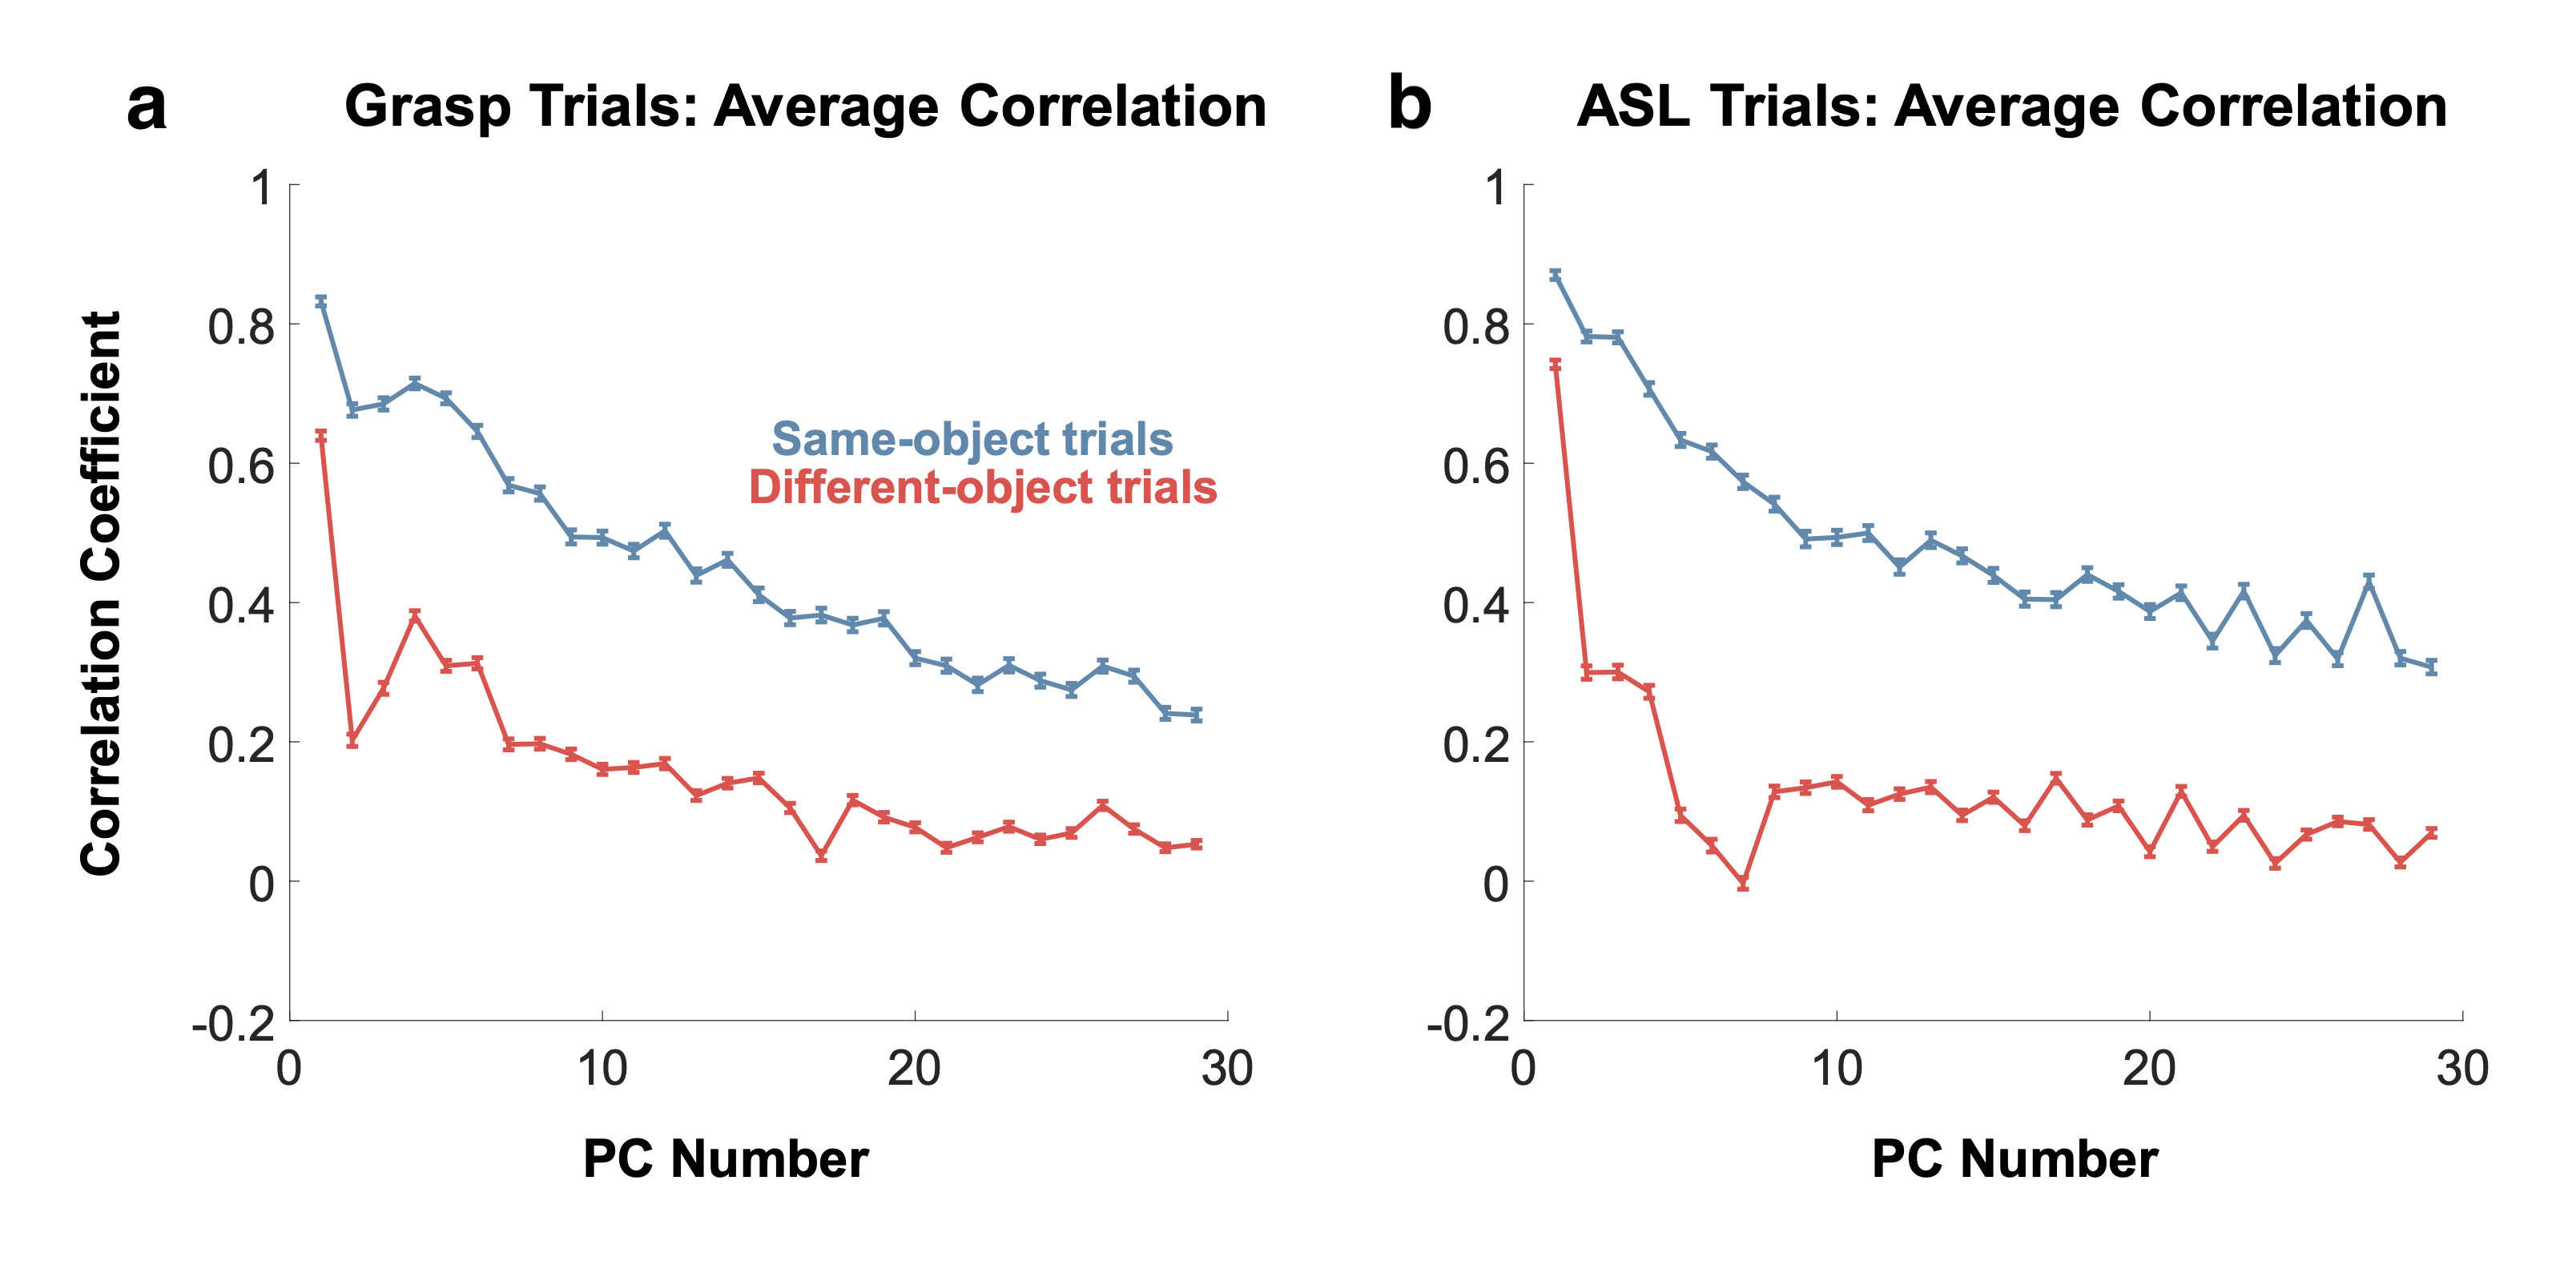
\includegraphics[width=1\textwidth,height=\textheight]{../images/physiology/background/low_variance_PCs.png}
\caption{Taken from Yan et al.~2020. Plots show mean correlations
between hand joint kinematic trajectories during grasp trials with the
same (blue) and different (red) objects (a) and ASL signs (b) projected
onto the same principle components. Correlations are averaged across 8
subjects. Within-object and within-sign correlations are systematically
higher than their shuffled counterparts. Error bars denote SEM. This
data supports the idea that low-variance components of kinematics data
contain task-specific structure rather than merely reflecting noise.
This is encouraging for our experiments, which hope to extend this idea
into careful analyses of task specific features of EMG data across
learning and in response to perturbations.}\label{fig:low_variance_PCs}
\end{figure}

\subsection{Coordinative Structures}\label{coordinative-structures}

Many studies have contributed to the concept of synergies as a
hard-wired organizing feature of the motor
system{[}@mussa-ivaldiMotorLearningCombination2000,@DAvella2003{]}.
However, these works tend to extrapolate from non-primate preparations,
particularly in the frog, and use tasks which are inherently
low-dimensional to explain covariance structure in primate and human
kinematic and electromyography
data{[}@giszterMotorPrimitivesNew2015;@gao2017{]}. That said, it would
be foolish to deny the existence of synergistic muscle coactivation even
at the structural level. Careful studies of force control by the
fingertips present a complex story of dimensionality of control in this
regime{[}@raczSpatiotemporalAnalysisReveals2013{]}. Constraints exist in
the architecture of the hand as well as its control system, though we
maintain that concept of synergies, especially in the context of
dexterous movement, is often presented as an oversimplification rather
than a mere simplification. We believe the story of the hand is more
complex.

Studies have attempted to quantify the number of effective degrees of
freedom of the hand with various methods. This has primarily been taken
to be the number of linear features which contain a desired level of the
original signal variance, where the signal is the joint angles of the
hand engaged in various
behaviors{[}@Ingram2009;@TodorovDimensionality2005{]}. These methods
have resulted in roughly 8 linear features of hand kinematics to solve a
variety of tasks, with subtleties found in inter-task and inter-subject
variations. Note that the motor repertoire is hardly high-dimensional
when compared to the dimensionality of the visual feature extraction
system{[}@yanUnexpectedComplexityEveryday2020{]}. A recent study found
that low-variance linear, kinematic components displayed significantly
higher correlation within condition (e.g.~grasp of a specific object)
than across condition. This suggests that these components carry
task-dependent information rather than condition-independent,
task-irrelevant noise{[}@yanUnexpectedComplexityEveryday2020{]}. This
suggests that the control of the hand is more nuanced than a set of
fixed synergies.

What Bizzi and colleagues call ``the problem of supraspinal pattern
formation''--how synergies are activated through time-- we argue, in the
context of hand control, is not simplified by the existence of
hard-wired or soft-wired
synergies{[}@bizziMotorPlanningExecution2020{]}. Rather, the CNS
produces control signals in a range of contexts and in response to
continually changing task demands. Rather than the CNS ``simplifying
movement'' through synergetic action, it is more likely that hand
synergies fall out of a optimization strategy which trades off effort
and accuracy where effort may, in part, correspond to independent
control of individual control dimensions. In this view, synergies,
hard-wired or not, reflect the statistics of the environment in which
movement is
constructed{[}@brutonSynergiesCoordinationComprehensive2018{]}. If we
limit ourselves to synergetic control, then we have simply passed the
problem to a lower-dimensional one of the same fundamental nature.
Neural control of the hand likely contains a spectrum of modularity in
order to maintain its role as a flexible instrument. Synergetic action
is one end of this spectrum resulting from the computations inherent to,
along with the structures of the human movement machine.

\subsection{Fractionating Structures}\label{fractionating-structures}

Just as many muscle fibers may be innervated by a single AMN, up to
thousands of neurons contact single AMNs through monosynaptic
corticospinal, or corticomotoneuronal (CM), connections and other
descending pathways through elaborate spinal circuitry. The hallmark of
CM connections in particular is their influence over multiple muscle
compartments as well as multiple muscles, though typically agonist or
antagonist sets{[}@cheneyFunctionalClassesPrimate1980{]}. This may seem
counter-intuitive as a means to produce individuated movement, but
experimental evidence in primates has shown that the convergence of many
CM collateral fibers onto single AMNs driving the distal muscles in
particular can produce a fine grading of activity over motor units
driving the distal joints. CM cells also appear to play a role in the
inhibition of antagonist muscles prior to contractions required for
movement {[}@griffinMotorCortexUses2020{]}. These findings confirm
theories about the excitatory and inhibitory role of these connections
dating back decades, and combine to suggest that variables encoded in
cortical ensembles are more complex than kinematics or dynamics
alone{[}@cheneyFunctionalClassesPrimate1980{]}.

The CM tract thus acts in coordination with synergistic muscle
activations of the hand to achieve control that is balanced between
modularity and flexibility. Findings suggest that there is a bipartite
structure in human motor cortex driving dexterous control of the distal
part of the upper limb which, it has been suggested, evolved under
pressure to quickly generalize between tasks. This work argues that
these two streams of hand control, namely ``fractionated'' and
``synergistic'' control, may interact to produce versatility, and
balancing these subsystems may be a key part of the optimization
function when learning new
skills{[}@Rathelot2009;@griffinCorticomotoneuronalCellsAre2015;@Takei2017{]}.
This dualism is likely not rigidly dichotomous, but rather a spectrum of
overriding fractionation (so-called ``New M1'') atop a phylogenetically
older system of synergistic
action{[}@dumCorticospinalSystemStructural2011{]}. Griffin and
colleagues found that CM cells are functionally tuned to a muscle's mode
of activity (agonist, antagonist, fixator) to ``bypass spinal cord
mechanisms and sculpt novel patterns of motor output that are essential
for highly skilled
movements''{[}@griffinCorticomotoneuronalCellsAre2015{]}. The hypothesis
stemming from the previously described work is that CM connections
override the ``consolidated'' patterns putatively generated via spinal
interneuron circuitry. The setup devised in our work aims to measure
fractionation by tracing motor unit correlations across learning.
Whether fractionation in our experiments is due to the CM pathway can
only be speculation, but our work may provide direction for future
studies pairing intracortical recordings with careful electromyography.

\subsection{Supraspinal Motor Maps}\label{supraspinal-motor-maps}

It is known from recent work that primary motor cortex (M1) is not an
isolated movement-generating dynamical system, but rather a node in the
network of a feedback-modulated, distributed movement
machine{[}@sauerbreiCorticalPatternGeneration2019{]}. Thinking of the
structural architecture of M1 as an input-driven system with outputs
along a spectrum of modularity from synergistic to fractionated, we can
ask what kind of functional architecture might have evolved in the
neuromuscular controller? Graziano and colleagues found that 500ms
electrical stimulation to M1 reliably produced stereotyped movements in
primates{[}@graziano2006{]}. These movements appeared to produce
goal-oriented actions pulled out of other contexts such as bringing food
to the mouth, and seemed to be arranged on the cortical sheet
topographically in terms of spatial endpoints rather than as a
humunculus. Graziano refers to this as the cortical ``action map'', that
these stimulations tapped into the control mechanisms of the primate's
motor system{[}@grazianoIntelligentMovementMachine2009{]}. These results
has recently been confirmed by optogenetics work in marmosets and
macaques {[}@ebina2019;@watanabeForelimbMovementsEvoked2020{]}.

The motor map concept suggests interpreting activity in M1 as a field of
feedback control microcircuits, integrating and transforming inputs,
both internal and external, to sculpt ongoing
movement{[}@wiltschkoMappingSubSecondStructure2015{]}. This is in
accordance with the idea that there is a structural hierarchy in M1
covering a spectrum of movement modularity. These ideas together form a
picture of the motor system as a structural scaffold upon which
behaviorally relevant feedback mappings from cortex to the spinal cord
are continuously activated and modulated based on information and
estimates about the periphery. In this view, the encoded variables of
interest depend on the goals, context, and perturbations of the intended
movement. \{+@fig:strick\_graziano\} shows Graziano et al.'s stimulation
results, what might be termed a functional view of the cortical motor
system, next Strick er al.'s described above clarifying the structural
view of modularity in this system.

\begin{figure}
\phantomsection\label{fig:strick_graziano}
\centering
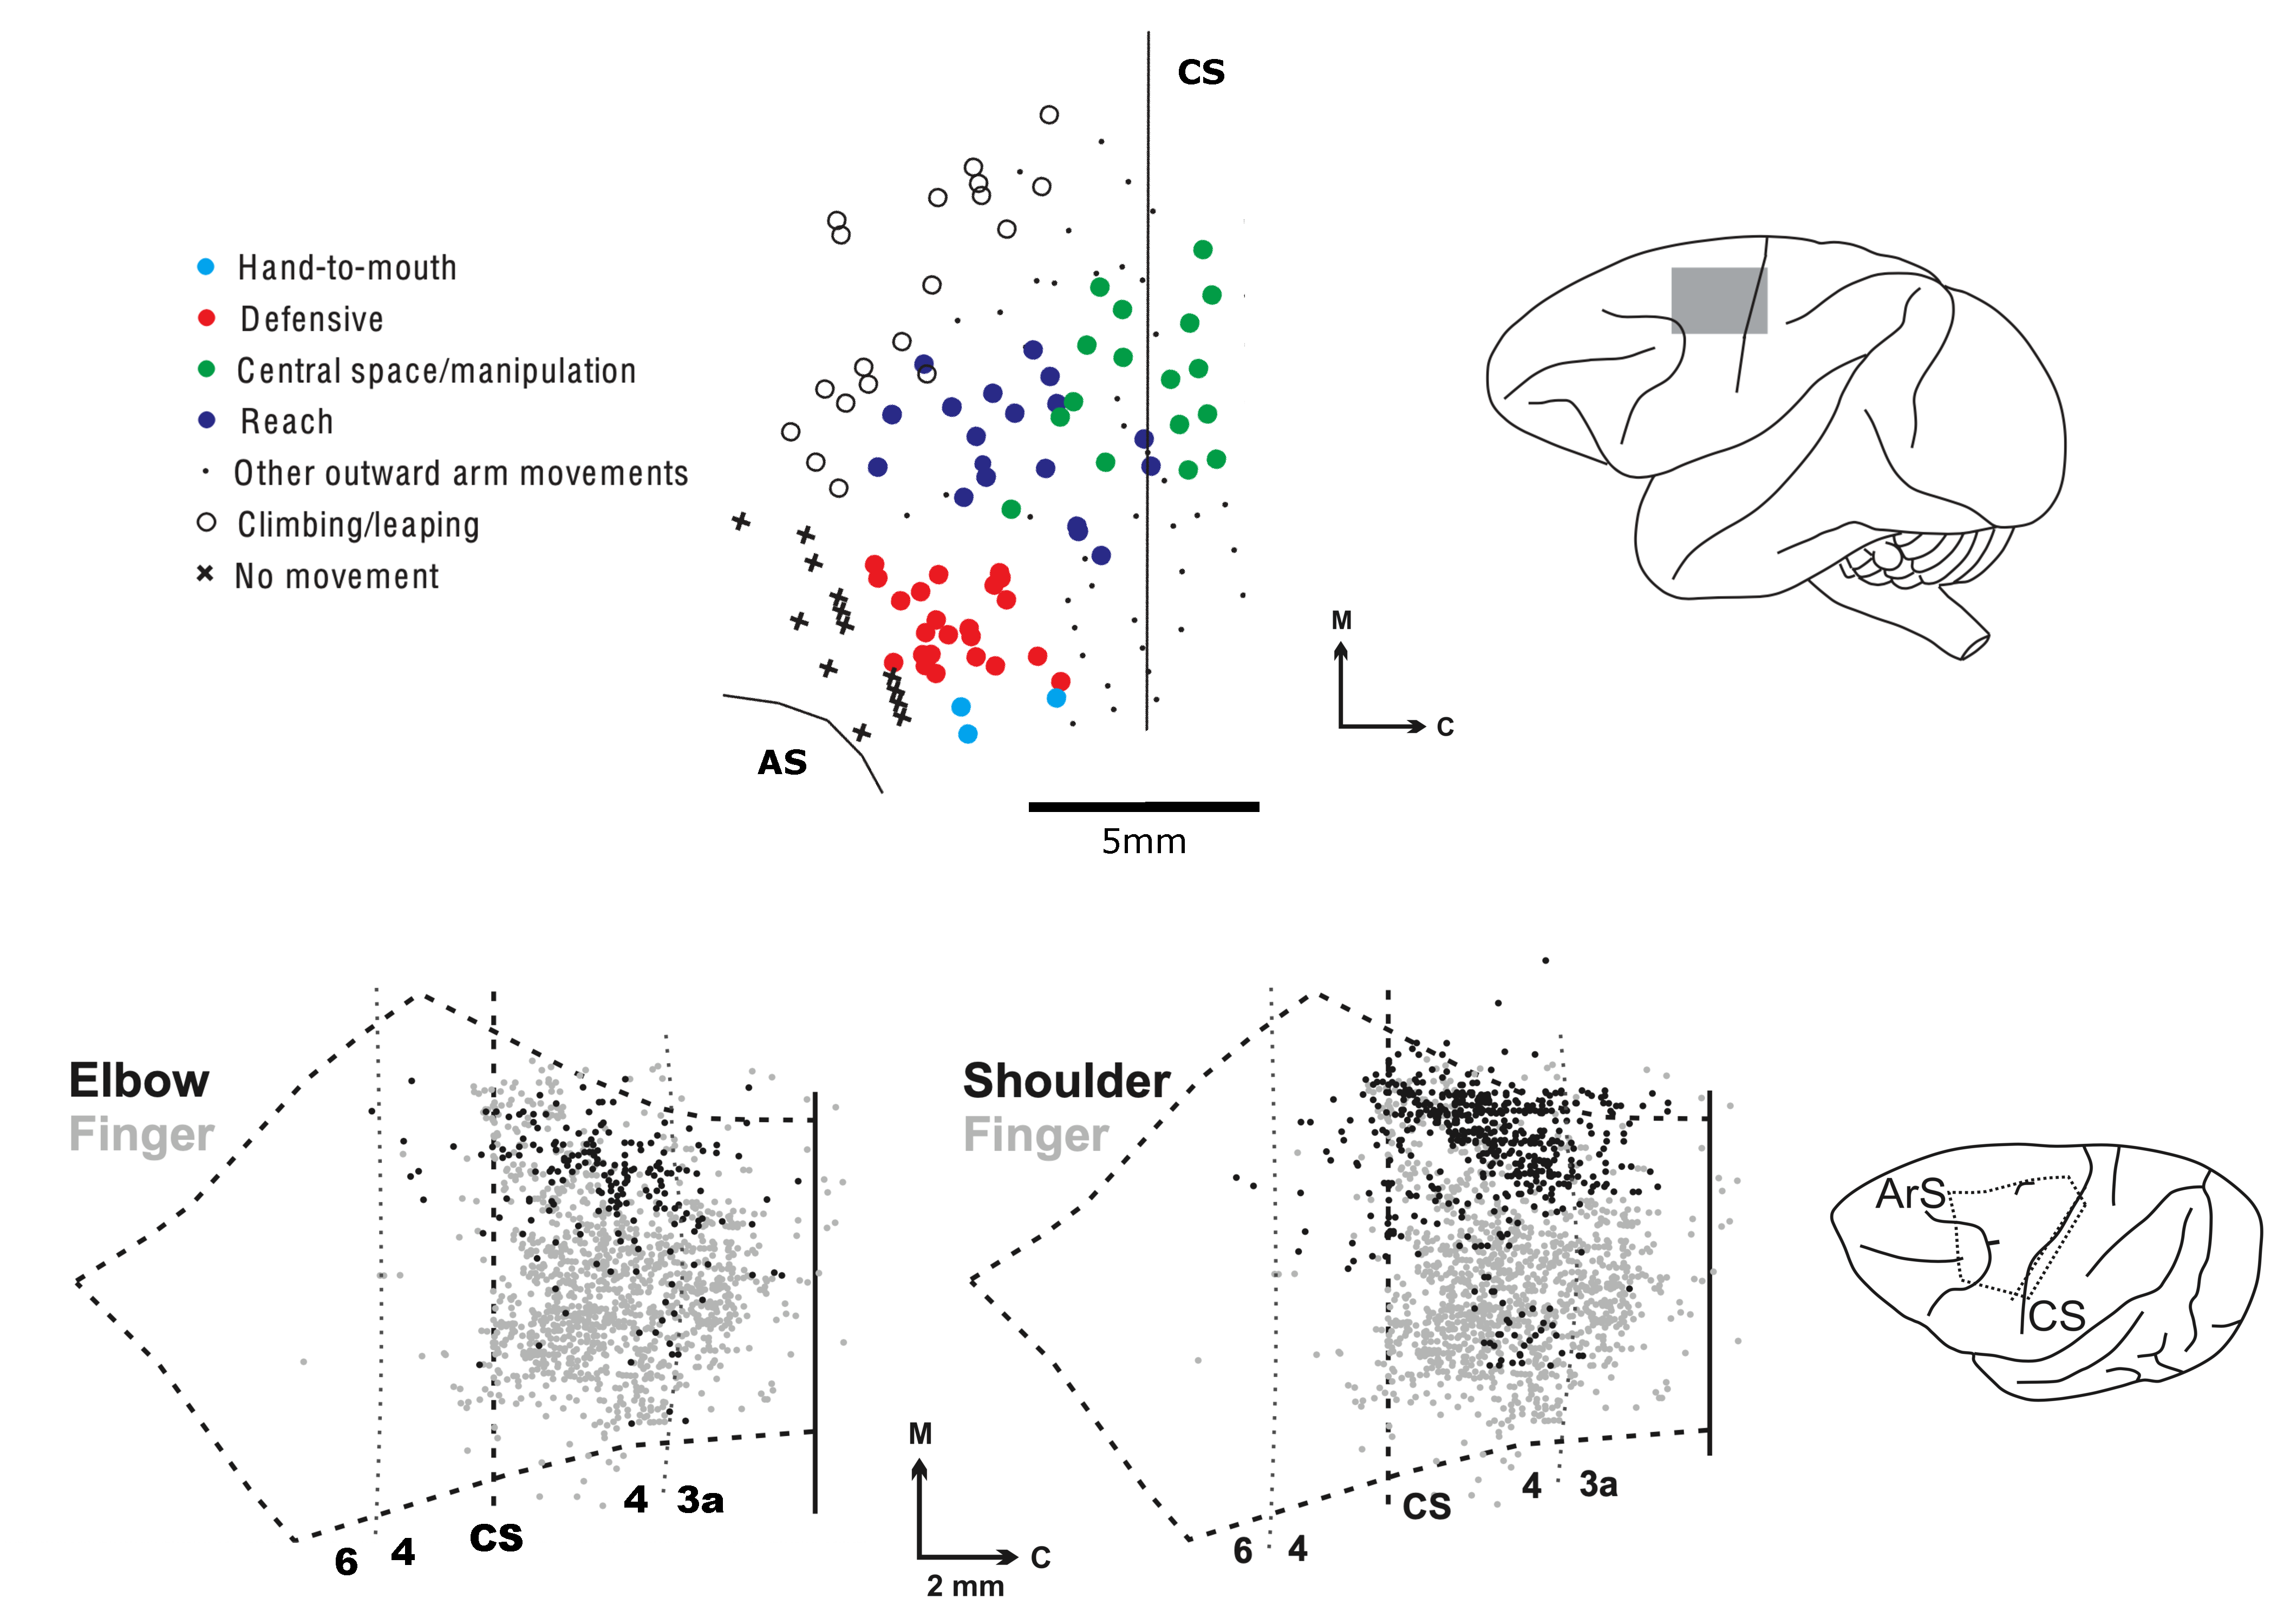
\includegraphics[width=1\textwidth,height=\textheight]{images/physiology/strick_graziano/strick_graziano.pdf}
\caption{Similarities between electrical stimulation on behavorial
timescales and rabies tracing identification of CM cells. CM cells are
largely confined to the caudal half of M1, while this region tends to
evoke complex manipulatory movements when electrically stimulated. (Top
Left) Corticomotoneuronal (CM) cells traced using rabies from muscles of
the elbow and finger. (Top Right) CM cells traced using rabies from
muscles of the shoulder and finger. (Bottom) Complex movements evoked by
500ms electrical stimulation pulse trains. Adapted from Graziano 2005
and Rathelot et
al.~2009{[}@graziano2005;@Rathelot2009{]}.}\label{fig:strick_graziano}
\end{figure}

Graziano writes:

\begin{quote}
``The usefulness of a feedback-dependent mapping from cortex to muscles
is that it can in principle allow neurons in motor cortex to control a
diversity of movement variables, such as direction, speed, hand
position, or posture that transcend a fixed pattern of muscle
activation. If the network receives feedback information about a
specific movement variable, then it can learn to control that
variable.''
\end{quote}

Muscle activity is, in this sense, a readout from a network transforming
state-dependent inputs into movement goals. Rather than choosing muscle
patterns in reconfigurable blocks, it creatively constructs and sculpts
movement. The hierarchy of the motor system may not be rigidly organized
around a particular set of variables. As shown in
\{+@fig:motor\_system\}, many loops exist connecting cortex with the
spinal cord, the cerebellum, the basal ganglia, and the sensorimotor
periphery. Each of these loops contributes information for the flexible
activation of the relevant action maps. Put simply, prevailing evidence
suggests that cerebellar loops provide predictive state information
while basal gangliar loops provide state and/or action value
information. Taken together, this work provides an image of the
incredible complexity which generates dexterous movements of the hand.
This is the foundation on which we can work to build experiments which
elucidate the computations involved in the production of skilled
movement. We aim to connect our results back to what is known about the
system we are attempting to reverse-engineer in order to inspire future
inquiries into the inner workings of the movement machine.

\begin{figure}
\phantomsection\label{fig:motor_system}
\centering
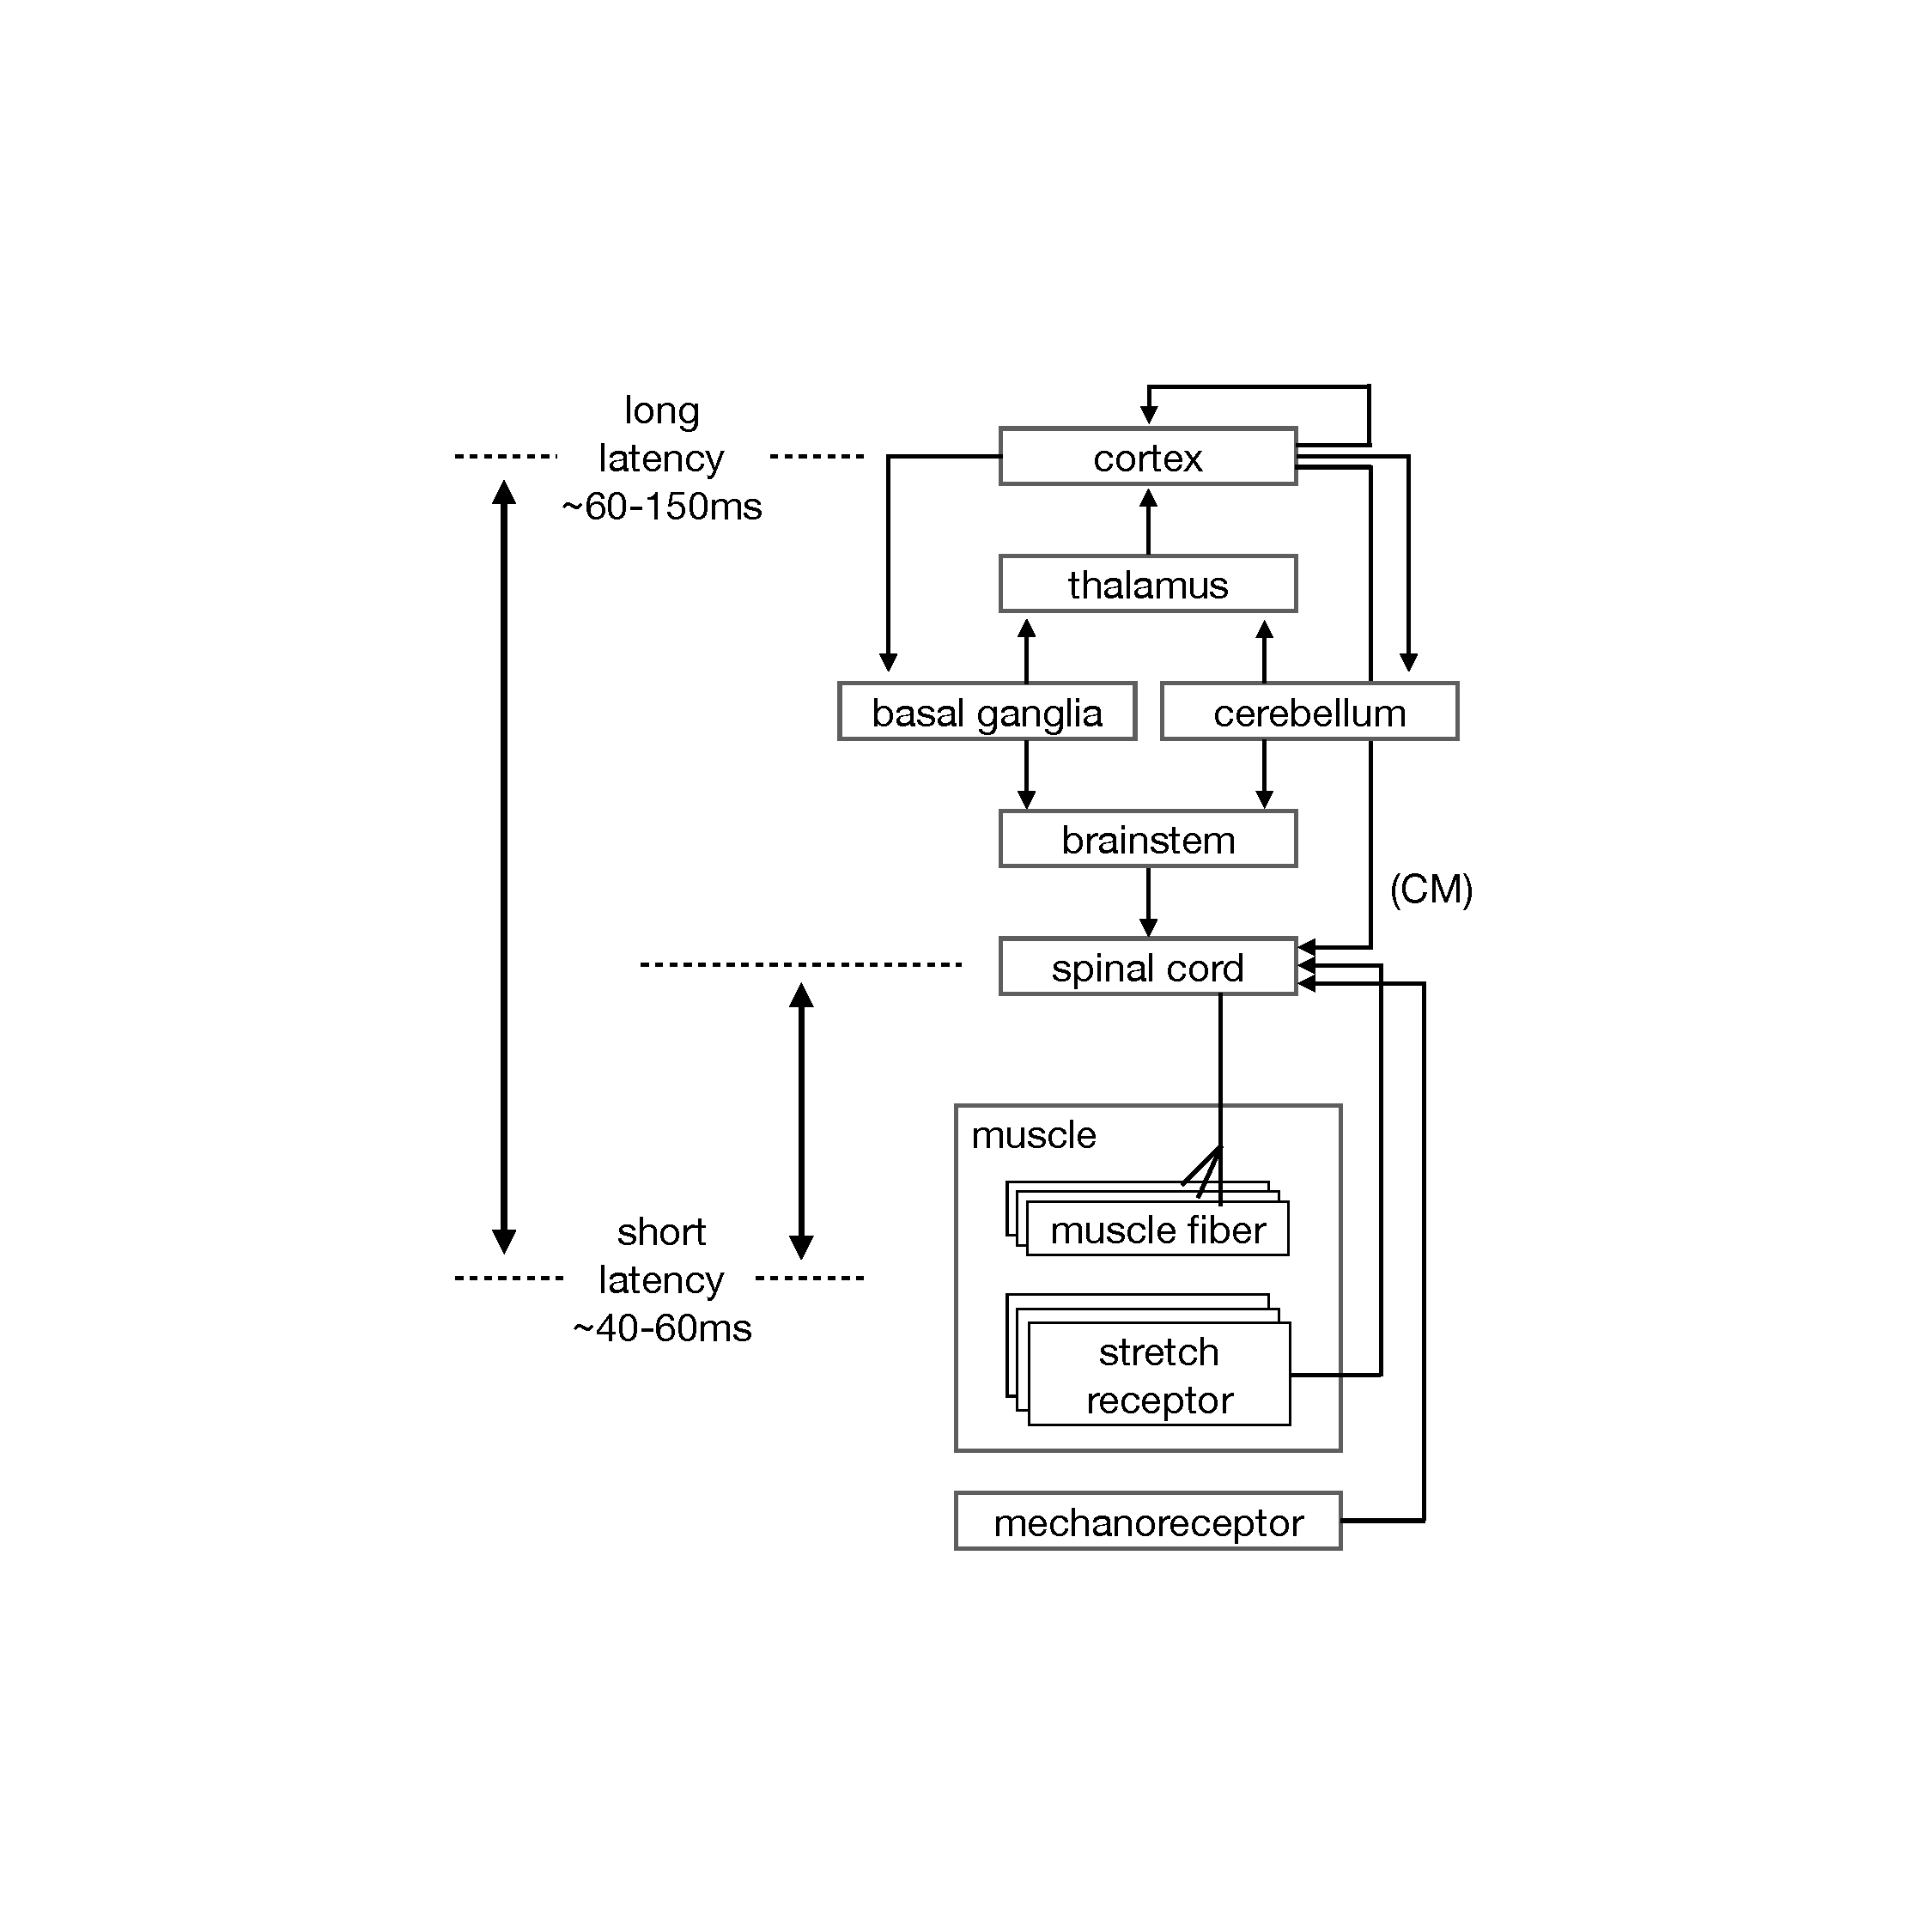
\includegraphics[width=1\textwidth,height=\textheight]{images/physiology/motor_system/motor_system.pdf}
\caption{Overview sketch of the motor system depicting the the
redundancy of the system both hierarchically (multiple muscle fibers are
innervated by the same motor neuron, many motor neurons innervate the
same muscle) as well as heterarchically (parallel spinal,
corticomotoneuronal, cerebellum, basal gangliar feedback loops).
Parallel reflex responses can be classified as long latency
(approximately 60-150ms) and short latency (approximately 60ms). We hope
to consider the parallelism and redundancy of the motor system to
inspire our data analyses and models of motor
computation.}\label{fig:motor_system}
\end{figure}

\subsection{John Rothwell and Jens Bo Nielson: Voluntary
Control}\label{john-rothwell-and-jens-bo-nielson-voluntary-control}

\begin{quote}
In the vast majority of cases, cortical inputs fi rst contact
interneurones which then relay the commands to motoneurones. Since the
same interneurones also receive con -tinuous input from sensory
receptors (and hence might be thought to participate in spinal refl
exes) as well as from interneurones from other parts of the spinal cord,
this means that by the time cortical input reaches motoneurones it has
been fi ltered by multiple lower level systems. In higher primates and
in man, cortical input can access some motoneurones via a special direct
pathway (the corticomotoneuronal pathway), which is often supposed to
play a critical role in volitional movement. However, even if this input
is strong (and there is little comparative evidence on this) the
excitability of motoneurones will have been biased by the multiple other
inputs that each one receives. Thus, even this connection does not
guarantee the brain a straightforward control of muscle.
\end{quote}

\begin{quote}
We argue that distributed cortical projections allow for flexibility of
connections between muscle representations, and therefore are critical
to the flexibility of movements unrestricted by postural demands.
Physiologically, the cortex is the main gateway for visual inputs to
enter and infl uence motor control. This is particularly relevant during
reaching with the arm and during the swing phase of gait for the leg. In
both cases, the limbs are relatively free from feedback control from
gravitational and contact force sensors, and can therefore be driven to
a large extent by visual inputs.
\end{quote}

Posture and contact dictates much of corticospinal function, and we
would expect that these demands influence the architecture of the
underlying circuitry. ``Conscious'' control is likely simply the
availability of visual and propriospinal sensation in the course of the
movement.

\begin{quote}
The anatomy and physiology of the {[}corticospinal{]} connections mean
that if a volitional command were formulated in some hypothetical
centre, it would be extremely diffi cult to predict the consequences
with any certainty unless the state of every interposed connection were
known in advance.
\end{quote}

Nielson argues that hierarchy doesn't function straightforwardly, that
all corticospinal loops can be seen as a collection of distributed,
overlapping modulation of motor neuron activity.

\begin{quote}
About 40 percent of the corticospinal fi bers come from the primary
motor cortex, whereas the cingulate and supplementary areas supply only
about 20 percent each and the premotor areas some 10 percent (Lemon,
2008). All of these areas of cortex also project to brainstem areas that
give rise to reticulospinal tracts, giving them an indirect, cortico-
reticulo-spinal route to the spinal cord as well as the direct
corticospinal route. The primary motor cortex is thought to have fewer
of these indirect connections than other motor areas, suggesting that
its output represents the most `favored' cortical access to spinal cord
circuits.
\end{quote}

\begin{quote}
In primates most of the terminations of the corticospinal tract are on
interneurones in the spinal grey matter with a smaller number of direct
monosynaptic inputs to motoneurones, particularly those inner-vating the
distal muscles of the extremities. These connections represent the only
way the cortex can interact directly with the motor apparatus
(corticomotoneuronal connections).
\end{quote}

\begin{quote}
after pyramidotomy {[}\ldots{]} movements remain slower and fatigued
more rapidly.
\end{quote}

This may be connected to synchronization of the CST? synchronous,
driving input for rapid reactions.

\begin{quote}
We do not know the rules that specify spinal organization in any detail.
However, one striking observation is that most of the connections
between sensory input and motoneurone output are indirect, going via
interneurones rather than direct sensory- motor pathways ( Jankowska,
2001; 2008). An obvious exception to this is the monosynaptic connection
between primary muscle spindle afferents and their homony-mous
motoneurones. However, this seems very much to be a special case rather
than the rule.
\end{quote}

\begin{quote}
One advantage of having interposed interneurones is that they are an
effective way of allowing the spinal circuitry to switch between
different states. For example, in the two funda-mental states of stance
and gait, connectivity during posture should be arranged in order to
resist perturbations of the body whereas during gait postural control
must be released and movement allowed. Going from posture to movement
means turning off the connections that assure stability and turning on
those that allow movement. {[}\ldots{]} A second advantage of
interneurones is that they can specialize in producing different
patterns or rhythms of activity. This could be a special property of
individual neurones or a property of an interconnected network of
neurones, such as envisaged for the locomotor pattern generator.
\end{quote}

Drawing a picture where spinal circuits are autonomous, but modulated,
by cortical input.

\begin{quote}
t is a general fi nding that every single interneu-rone receives input
not only from the sensory modality which is the basis for its classifi
cation (e.g.~as a `Ia inhibitory interneurone', `Ib inhibitory
interneurone', `gr. II interneurone' or `fl exor refl ex afferent
interneurone'), but also from a number of other sensory afferent
modal-ities, other interneurones and a number of descending pathways
(e.g.~corticospinal, vestibu-lospinal, reticulospinal).
\end{quote}

\begin{quote}
It is not an unrealistic possibility that spinal interneurones with a
slight turn of events could have been classifi ed based on their
supraspinal input as taking part in different voluntary movements rather
than the current clas-sifi cation based on afferent input as taking part
in different refl ex actions. This was realized already by Sherrington
(1906) more than 100 years ago when he wrote: ``A simple refl ex is
probably a purely abstract conception, because all parts of the nervous
system are connected together and no part of it is probably ever capable
of reaction without affecting and being affected by various other parts,
and it is a system certainly never absolutely at rest. But the simple
refl ex is a convenient, if not a probable, fi ction.''
\end{quote}

\begin{quote}
\textbf{The discharge of every single motoneurone and thus the
activation of every single muscle fi ber is determined by the integrated
depolarization from on average 10,000 synaptic inputs arising from a
number of different sensory modalities, spinal interneu-rones and
supraspinal control centres.}
\end{quote}

\begin{quote}
Cortical input to the spinal cord should be viewed as using or
modulating the output of the spinal circuitry itself. There is no
separation between `spinal refl exes' and `cortical voluntary movement'.
Instead, it is important to focus on how the neuronal machinery in the
spinal cord may provide an extremely fl exible tool for the execution of
voluntary movements.
\end{quote}

\begin{quote} 
  We hypothesize that there are at least two advantages of cortical control. The fi rst is adaptability which emerges as a consequence of the anatomy of the cortical motor representation. The second is integration of visual input which is particularly important in shaping the hand to manipulate objects. Individuation and precision are secondary consequences of this organization.
\end{quote}

Begs the question of a no-visual experiment?

\begin{quote}
  EMG recordings show that very short synchronous bursts of activity are characteristic of many fractionated fi nger movements, such as writing and tool use {[}\ldots{]} Interposing interneuronal synapses in these connections would tend to remove synchrony and smooth out the command. This is indeed what is seen following corti-cospinal lesion (Farmer et al., 1993). The CM system may thus also be at the heart of human evolution in view of the evolutionary advantage of being able to throw something at an animal in order to kill and eat it.
\end{quote}

\begin{quote} 
  One- third of the cortex, particularly in the parietal and premotor areas, is devoted to visual processing. A considerable part of this is used for shaping/orienting our hand in preparation for grasping and manipulating objects
\end{quote}

\begin{quote} 
  the motor cortex may differ from the spinal cord in degree of fl exibility and a larger possibility of integrating visual input, but otherwise there are no differences between the motor cortex and the spinal cord circuitries (after all CM cells project to motoneurones and receive sensory input much like any good old- fashioned interneurone) that could warrant a signifi cantly different role in our conscious experience of control of the movements that we perform. What we are proposing is that it is not the degree of perceived volition which determines to what extent the motor cortex is involved in a given task, but rather the need for fl exible visual control.
\end{quote}

\begin{quote} 
  We hope that we have made it clear that there is little to support this distinction between automatic and voluntary tasks. We need to consider the integration between supraspinal and spinal control centers for any specifi c task in order to understand how that task is controlled by the nervous system, and try to avoid putting into it volition and voluntary which in any case are terms that belong in philosophy or in specifi c inquiries aimed at unravelling the mechanisms of our cognitive abilities and our conscious experiences.
\end{quote}

Compelling case to look at the entirety of the system, focusing on the contributions that cause motor neurons to fire.


\section{Mathematical Theories of Motor Control and Learning}
  
  What are ``normative models''?
  
  \begin{quote}
  Normative models suggest that the nervous system optimally adapts when
  faced with an error. To determine this optimal adaptation, the normative
  model must specify two key features of the world. First, how different
  factors, such as tools or levels of fatigue, influence the motor system
  --- the so-called generative model. Second, how these factors are likely
  to vary over both space and time --- that is the prior distribution. The
  structure of the generative model and the prior distribution together
  determine how the motor system should attribute an error to the
  underlying causes and, therefore, how it should adapt.
  {[}@wolpertPrinciplesSensorimotorLearning2011{]}
  \end{quote}
  
  \$include includes/ofc.md
  
  <!-- OFC MODELING AND DISCUSSION -->
  $include includes/ofc.md
  
  <!-- MODEL ADAPTATION VIA GRADIENT DESCENT -->
  $include includes/model_adaptation.md
  
  
  <!-- 
  
  adaptive is within trial, as you move
  episodic has endless access to a simulator
  
  ## List of variants, etc 
  
  - LQR + SDN
  - robust control (?)
  - KL-control + composition
  - game theoretic control-- compare solutions
  
  ## Distributed Control
  
  > The hierarchical organization typical of earlier sensory areas is not adhered to everywhere. On the contrary, the anatomy of associative areas and prefrontal  cortex suggests a more "democratic"  organization, and  processing  appears to take place  in webs of strongly interacting networks (8). Decisions to act and the execution of plans and  choices  could be the outcome of a  system with  distributed control rather than  a single control center. Coming to grips  with systems having distributed control will require both new experimental techniques and new  conceptual advances. Perhaps more  appropriate  metaphors for this  type of processing will emerge from studying  models of interacting  networks of neurons. [@sejnowskiPerspectivesCognitiveNeuroscience1988]
  
  ## Policy Selection
  
  each timestep you combine actions from component policies to choose an action
  
  Here we'll review and discuss models of action selection and policy composition as a means of theorizing about how subjects learn novel skills. 
  
  In a sense, we're setting up several different directions for our understanding of composition and action selection which can be experimentally tested. 
  
  We have a direct selection algorithm, composition through policy addition, and composition through policy multiplication. 
  
  
  ### KL-control Composition (1 day)
  
  This setup is particular subset of OFC problems. 
  
  Dynamics
  Cost
  
  Composable policies
  
  PLOT OF INTUITIVE EXAMPLE
  
  ### Multiplicative Policy Composition
  
  Policies are distributionally weighted, as opposed to chosen each timestep? 
  
  ### Temporal Composition
  
  there is a spectrum of latency in the feedback response
  
  can different controllers be used for different latencies, and adjusted accordingly?
  
  ### Generalized Policy Selection (1 day)
  
  This is in the MDP case
  
  Learning happens in several ways-- reward regression, Q-learning
  
  What are rewards? 
  What are tasks?
  What are actions?
  
  Is GPI with LQRs / LQR-RL a good model for motor learning? Define a model and see if it recapitulates known motor learning phenomena on existing experiments + accounts for things that previous models don’t. (Similar in spirit to Geerts et al. (2020)). Can this model track the higher-order statistics of trajectories during motor learning?
  
  ### Model-based Reinforcement Learning
  
  Since we only have an approximate model of the system dynamic, we could simply work towards an optimal policy directly using gradient derivative-free optimization methods in a model-free approach. Since we have good evidence that humans leverage internal models to make decisions (at least in a motor problem domain), we need to define an algorithm which uses past observations and controls to update our approximation for the system dynamic. Here is a very general algorithm:
  
  0. Define a base policy/controller and base system model ($L_0$ and $\hat{M}_0$)
  1. Collect samples (by interacting with the true environment $M_{true}$) using the current policy/controller (collect $y_t,u_t,y_{t+1}$ triples using $L_i$ for $i \in \{0\dots N\}$
  2. Use sample(s) / trajectories to update current system dynamical model $\hat{M}_i$
  3. Update current policy/controller $L_i$ (using the system dynamics or using a direct policy method)
  
  If the true system dynamics were known, we could solve the Algebraic Riccati Equation with a backwards pass, and compute our controls in a forward pass. This general algorithm structure highlights how the (unknown) system identification and controller design are intertwined: identifying a system appropriately must rely on sampling and fitting regions of the state space pertinent to adequate control in terms of cost (Ross ICML 2012). Otherwise, our approximation to the true system dynamic will only produce a valid controller in regions we have previously explored. The question is how we can effectively (sample and time efficiently) utilize new state transitions we encounter either online as feedback or between trials to update our model and policy. That is, the number of trials and/or trajectories to use before updating either the system model and/or policy is an important parameter.
  
  In the LQG setting, this might be called "adaptive LQG".
  
  \$include includes/model\_adaptation.md
  
  Learning LQR controllers
  
  \begin{verbatim}
  Q-learning for LQR
  policy gradient for LQR
  what is an LQR-SR? what does this help us do?
  \end{verbatim}
  
  where does LQR break? - goal shift (is this true?) - task shift
  (different goal? this isn't true) - goal uncertainty (this can't be
  modeled\ldots) - LQR variants break more easily?
  
  where does KL-LQR / control break? - one policy at a time\ldots?
  re-optimize your single policy per task? (task could have multiple
  goals) - could have multiple possible (terminal) goal states - not
  continuous -- code this up and understand it in continuous would be a
  good result - selection is done beforehand\ldots{} can this shift
  online\ldots? - allows you to construct more interesting
  policies\ldots{} - can we connect this to KL between passive and
  dynamic? change this to planned and replanned?
  
  is there a multiplicative LQR composition? - sergey levine
  multiplicative paper?
  

# motor learning

## random 

The brain seems a thoroughfare for nerve-action passing on its way to the motor animal. It has been remarked that Life’s aim is an act, not a thought. Today the dictum must be modified to admit that, often, to refrain from an act is no less an act than to commit one, because inhibition is co-equally with excitation a nervous activity. (Sherrington, Rede Lecture, 1933)


## kitano robustness [@kitanoBiologicalRobustness2004]

Robustness is a property that allows a system to maintain its functions despite external and internal perturbations. 

A system must be robust to function in unpredictable environments using unreliable components. 

Robustness is ubiquitous in living organisms that have evolved. 

Robustness is the maintenance of specific functionalities of the system against perturbations, and it often requires the system to change its mode of operation in a flexible way. In other words, robustness allows changes in the structure and components of the system owing to perturbations, but specific functions are maintained.

The mechanisms that ensure the robustness of a system are system control, alternative (or fail-safe) mechanisms, modularity and decoupling.

System control consists of negative and positive feedback to attain a robust dynamic response observed in a wide range of regulatory networks

Robustness can be enhanced if there are multiple means to achieve a specific function, because failure of one of them can be rescued by others. Here, I call this mechanism ‘alternative’, or ‘fail-safe’. This concept encompasses redundancy, overlapping function and diversity, as the differing degrees of similarity between the various alternative means that are available.

Redundancy generally refers to a situation in which several identical, or similar, components (or modules) can replace each other when another component fails. Diversity, or heterogeneity, represents the other extreme, whereby a specific function can be attained by different means available in a population of heterogeneous components. 

Modularity is an effective mechanism for containing perturbations and damage locally to mini- mize the effects on the whole system. Modules are widely observed in various organisms, functioning as possible biological design principles

Decoupling isolates low-level variation from high-level functionalities.

**My theory is that robustness is an inherent property of evolving, complex dynamic systems — various mechanisms incurring robustness of organisms actually facilitate evolution, and evolution favours robust traits. Therefore, requirements for robustness and evolvability are similar. This implies that there are architectural requirements for complex systems to be evolvable, which essentially requires the system to be robust against environmental and genetic perturbations.**





## psychology of reaching 2020

Behavioral studies have provided further support for the parallel planning hypothesis. In these studies, an initial display shows potential targets, and the participant must initiate a movement prior to final target specification. Under such conditions, the initial movement direction corre- sponds to a weighted average of the potential movements

Behavioral studies have also offered a reconceptualization of the initial trajectories observed in tasks involv- ing goal uncertainty (Wong & Haith 2017). Rather than indicating an averaging process, these trajectories may reflect a deliberate decision regarding how to optimize performance (Hudson et al. 2007). That is, an intermediary trajectory may be optimal to rapidly update a (single) move- ment plan once the final goal is specified. When this option is no longer optimal—for example, by increasing the distance between candidate targets—the occurrence of intermediate movements is dramatically diminished (Figure 2d) (Haith et al. 2015a).

The probability of intermediate movements increases when targets overlap in terms of semantics (Dale et al. 2007), phonology (Spivey et al. 2005), or even truth evaluation (McKinstry et al. 2008). These effects suggest that interference in goal selection may promote an optimal strategy to plan an intermediate movement without committing to the final goal. 

*cognitive strategies-- reflects optimality given cost of controlling arms, etc independently.*

Decision making is a dynamic and multilevel process that encompasses multiple brain networks (Gallivan et al. 2018). It entails the evaluation of the value associated with possible options (Padoa- Schioppa 2011), constrained by the current context. Decision-making processes continue to oper- ate throughout the movement (Wispinski et al. 2018); we can change our minds after movement initiation, replacing one movement with another (van den Berg et al. 2016) or rapidly aborting an initiated movement (Verbruggen et al. 2019). It is reasonable that the optimal decision to make an intermediate movement amid uncertainty takes advantage of our capability to move in a flexible manner, as the ongoing behavior entails the continuous reevaluation of how our actions conform to current goals.

*flexibility is to continuous updating of ongoing plans, re-planning, etc, adjustment in face of changing environment and goals* 

The activity of neurons in premotor and motor cortices can be quite distinct during preparatory and execution phases (Figure 3d), and at the population level, the correlation is modest (Churchland et al. 2010).

Humans exhibit a rich repertoire of movements that vary in extent, speed, duration, force, and so forth. Despite this flexibility, there are notable features that remain largely invariant. After deciding to eat a cookie, our movement to that goal is not arbitrary: The hand smoothly follows a direct, rather than curved, path to the cookie, even though this may require rather complex, nonlinear changes in joint space (Morasso 1981). Moreover, the velocity profile is bell shaped, reaching a maximum around the middle of the movement. 

A hallmark of skilled behavior is a reduction in variability (Shmuelof et al. 2012b)

### feedback, online control

Feedback mechanisms are frequently described as reflexive, in the sense that they operate out- side awareness or volitional control. These mechanisms are divided into two components. First, there are reflexive responses of spinal origin. With latencies as short as 25 ms, sensory information from the muscles, joints, and skin can modify activity in motor neurons. This sensory informa- tion is integrated with descending motor commands by spinal interneurons to assist voluntary drive to the motor neurons to help correct or resist movement errors (Nielsen 2004, Pruszynski et al. 2009). [...] Second, there are more flexible, task-dependent long-latency reflexes, which are under the control of both subcortical and cortical mechanisms (Scott et al. 2015). Long-latency reflexes in response to mechanical perturbations have estimated latencies of 50 to 105 ms (Pruszynski & Scott 2012), whereas the response to visual errors ranges from 150 to 200 ms (Carroll et al. 2019, Day & Lyon 2000, Franklin & Wolpert 2008). 

[OFC] provides a unified framework to account for the relationship between planning and control: Con- trol mechanisms enacted during movement are a natural corollary of how reflex gains are set in a task-dependent manner prior to movement initiation. OFC also offers a solution to the degrees- of-freedom problem. Specifically, the brain tends to find a stereotypical manner of producing a movement because reflex gains are set in order to minimize task-relevant variability.

As might be expected, directing attention to the target improved performance when the tar- get was displaced. Interestingly, directing attention to the cursor had little impact on performance when the cursor was displaced. The authors (Reichenbach et al. 2014) hypothesize that the motor system retains a stable estimate of hand position regardless of attention. In addition, when the display included multiple moving targets and cursors, most of which were task irrelevant, the par- ticipants had difficulty identifying task-relevant target displacement amid the visual distractors. However, they were able to ignore these distractors when responding to feedback about hand position. It may be that proprioceptive feedback from the hand is readily combined with visual information to create a stable representation for feedback control. In contrast, vision provides the only source of feedback for responding to errors in the estimate of target position.

*Shows that the hand position representation is probably strongly dependent on proprioception. Does this remain when we make isometric contractions? I might expect the hand to have more haptic feedback than proprioceptive...?* 

Carroll et al. (2019) asked how properties of the target it- self, specifically reward value, affect online control processes. Participants initially reached toward a center target that was flanked by two outer targets. Immediately following movement initiation, but prior to a cursor jump, a cue was given to indicate which one of the three targets would be rewarded. Feedback responses beginning 170 ms post cursor jump reflected rapid computations normally associated with high-level decision-making processes, as the hand moved toward the rewarding target. 

*Not sure what's going on here-- unknown reward and a cursor jump?*


### error adaptation

Historically, [the term sensorimotor adaptation] was used to refer to an implicit and automatic learning process that keeps the motor system well calibrated. However, recent research has shown that adaptation is not a unitary process. Thus, we use the term in a more general sense, encompassing the many learning processes that allow us to flexibly modify skilled behaviors to be well suited for a range of contexts.


trial-by-trial state space model of error adaptation

\begin{align*}
e(n) &= r(n) - x(n) \\ 
x(n+1) &= Ax(n) + Be(n)
\end{align*}}

\begin{align*}
x(n+1) &= (A - B)x(n)+ Br(n)
\end{align*}

If training is limited to one part of the workspace, the generalization function is relatively narrow, showing a Gaussian-like function with a standard deviation of approximately 30° (Krakauer et al. 2000, Shadmehr & Moussavi 2000).

*Howard et al 2015 suggests that follow-through necessitates distinct motor plans, as subjects without follow-throughs failed to adapt to opposing force fields which changed on a per-trial basis.*

Several studies have shown that savings is almost entirely due to recall of explicit strategies (Haith et al. 2015b, Huberdeau et al. 2015, Morehead et al. 2015). In contrast, the implicit recalibration component does not increase across repeated exposures to the same perturbation, and even exhibits attenuation (Avraham et al. 2020).


### cerebellum 

In terms of a process-based account, the core deficit [as a result of cerebellum damage] has been associated with an inability to generate an accurate prediction of the sensory consequences of a movement, an impairment that not only disrupts learning but also underlies the dysmetric movements characteristic of ataxia (Wolpert et al. 1998).

In general, cortical areas including the prefrontal, parietal, and premotor cortices are strongly engaged during the early stages of learning, and exhibit a decrease in activity as performance improves (Bédard & Sanes 2014, Bernardi et al. 2018, Graydon et al. 2005, Krakauer et al. 2004, Shadmehr & Holcomb 1997). Regions within the cerebellum sometimes show a similar pattern (Bernard & Seidler 2013; Imamizu et al. 2000, 2003; Nezafat et al. 2001), consistent with the observation that cerebellar and cortical activity patterns tend to be positively correlated. However, increased activity within subregions of the cerebellum over the course of learning has also been reported (Graydon et al. 2005, Krakauer et al. 2004, Shadmehr & Holcomb 1997). These increases have been interpreted to reflect the establishment of a new internal model or recalibration of an existing internal model (Imamizu et al. 2000).

### implicit, explicit, use-dependent

[Consider] the error components when aiming at the landmark. Given the 45° rotation, the cur- sor lands in the target when reaching to the neighboring landmark. Despite this success, there remains, at least from the perspective of the motor system, a 45° sensory prediction error: The system generates a prediction of the sensory consequences (i.e., feedback at the landmark), but the cursor appears at the target. The recalibration process applies its update rule (see Equation 2), producing the observed drift function. Indeed, the drift would suggest that implicit learning over- rides strategy use.

Whereas adaptation is driven by SPE, the difference between predicted and actual feedback, strategy change is driven by target error (TE), the difference between the actual feedback and the goal 

**The computational goal of the implicit component of adaptation is to keep the motor system well calibrated, ensuring that motor commands are faithfully implemented (Miyamoto et al. 2020). This system appears impervious to information about task success. In contrast, the computational goal of a strategic process such as aiming is to ensure that the appropriate action is selected to optimize performance. For this to occur, it is essential to monitor how well a selected action achieves its desired goal.**

A striking example of UDL comes from a transcranial magnetic stimulation (TMS) study look- ing at motor cortex plasticity. At the beginning of the session, the TMS coil was positioned over M1 to elicit adduction of the thumb. The participant was then given the simple task of repeat- edly abducting the thumb. Post training, the same M1 stimulation now elicited thumb movements clearly shifted in the direction of abduction (Classen et al. 1998; see also Mawase et al. 2017).

a recent paper suggests that a bias to repeat recent movements may reflect constraints in action planning (Marinovic et al. 2017). These biases become diminished when participants are given more time for movement preparation; conversely, preparation for the repeated movement becomes more rapid (Mawase et al. 2018).

### RL 

Can binary feedback be sufficient to learn a visuomotor rotation? Izawa & Shadmehr (2011) provided salient positive feedback in the form of an exploding target for movements that fell within a window corresponding to roughly the magnitude of normal motor variability. This window was originally centered around the target but was gradually rotated, eventually reaching 8° away from the target. Behaviorally, participants were able to track the rotation from the binary feedback. However, learning was much more variable than that observed with standard, vectorial feedback, suggesting an exploratory process (Cashaback et al. 2017, Therrien et al. 2018). Moreover, tests of perceived hand position indicated that, unlike SPE-driven learning, the sensorimotor map was unchanged by binary feedback.

One hypothesis is that reward information has little effect on the rate of learning, but strengthens retention (Galea et al. 2015, Shmuelof et al. 2012a; for a different perspective, see Nikooyan & Ahmed 2015), on the basis of the observation that participants who received rewards during a visuomotor rotation took longer to wash out than those who did not receive rewards. However, Codol and colleagues (Codol et al. 2018, Holland et al. 2018) reported that the maintenance of asymptotic performance during washout was under participants’ explicit control; thus, the effect of reinforcement may be to make strategy use more salient, rather than have a direct effect on an internal model.

*skin-in the game type explanation*

If a target jumps mid-reach such that a rotated cursor lands within the target, adaptation is attenuated (Leow et al. 2018). One interpretation of this effect is that having the cursor land in the target results in a reward signal, which moderates the effect of the SPE (Reichenthal et al. 2016). Presumably the “reward” occurs even though the participant is fully aware that the outcome was not the direct result of his movement.

### questions

**How do we bring together computational ideas concerned with addressing high-level task requirements (e.g., where and when to move) with lower-level requirements needed to generate the motor commands that activate the appropriate muscles?**


## piano performance 

In piano performance, for keystrokes with each of the four fingers during playing various tone sequences, the hand kinematics was characterized by three distinct patterns of finger joint coordination (Furuya et al., 2011a). The motion of the striking finger was consistent across these patterns, whereas the motion of the non-striking fingers differed across them. This was interpreted as evidence for the independence of movements across fingers. In addition, the amount of movement covariation between the striking and non-striking fingers was similar, independent of which finger was used for a keystroke. The finding was in contrast to non-musicians who displayed a hierarchy of independence of finger movements, the middle and ring fingers being less individuated than the index and little fingers (Häger-Ross and Schieber, 2000; Zatsiorsky et al., 2000). The equal independence of movements across fingers can be therefore achieved by extensive piano training. This idea is supported by superior independence of finger movement control for pianists as compared to non-musicians (Slobounov et al., 2002; Aoki et al., 2005), which possibly occurs due to changes at biomechanical and neural levels (Chiang et al., 2004; Smahel and Klimová, 2004). (Shinichi Furuya* and Eckart Altenmüller 2013)



## bizzi review of sensorimotor loops

<!-- Extracted Annotations (31/12/2020, 15:58:46)

"A major function of these synergies is to simplify the control of movements, a notoriously hard computational problem" (Bizzi and Ajemian 2020:1815)

"question of control" (Bizzi and Ajemian 2020:1815)

"the overarching" (Bizzi and Ajemian 2020:1815)

"how are these building blocks coordinated in time by the supraspinal system to generate goal-directed movements?" (Bizzi and Ajemian 2020:1815)

""we have some idea as to the intricate design of the puppet and the puppet strings, but we lack insight into the mind of the puppeteer" (Bizzi and Ajemian 2015)." (Bizzi and Ajemian 2020:1815)

"how are they influenced by motor skill learning" (Bizzi and Ajemian 2020:1816)

"far more speculative and difficult to find are detailed proposals as to how, even assuming the existence of synergies, the CNS manages to generate effective control signals, a problem we refer to as the problem of supraspinal pattern formation." (Bizzi and Ajemian 2020:1816)

"By "perspective of sensorimotor loops" the following is meant: 1) synergies likely constitute the fundamental building blocks for movement control, and their patterned recruitment is largely dictated by the cortical output regions that give rise to the corticospinal tract; 2) there exist multiple sensorimotor loops involving the cortex, other brain regions, the spinal cord, and the sensorimotor periphery, all of which include these cortical output regions along their path; 3) each of these loops serves distinct, yet crucially overlapping, functional roles in solving the supraspinal pattern formation problem; 4) the continuous convergence of these loop activities at the cortical output regions engenders the emergence of functionally appropriate movement commands by shaping both loop activity and motor output activity; and 5) the mathematical perspective from which to view this phenomenon is that of distributed representation and distributed control in a complex multiscale system (Kitano 2004)." (Bizzi and Ajemian 2020:1816)

"even a simple movement is a global body event." (Bizzi and Ajemian 2020:1816)

"two recent papers employing this type of approach provide evidence that preparatory activity is far from being an early indicator of movement-related activity and, instead, reflects a separate but facilitating computation. Elsayed et al. (2016) showed that at the population level preparatory and movement activity occupy orthogonal subspaces, although a simple transformation relates the two, suggesting that preparatory activity is crucial for putting the system in a state that enables the dynamic evolution of movement commands." (Bizzi and Ajemian 2020:1817)

"Although the dynamical systems approach has, in certain respects, been an improvement over the representational approach in understanding the role of preparatory activity, it too has shortcomings: dimensional reduction techniques make the relevant "variables" difficult to interpret and inconsistent from one study to the next; recording from dozens of neurons simultaneously is an improvement over recording from a single neuron but still falls orders of magnitude short of the number of neurons involved; and, in contrast to a feedback view of movement, the dynamical systems approach generally suggests that once a movement is prepared, motor cortical dynamics alone govern how movement dynamics unfold" (Bizzi and Ajemian 2020:1817)

"Kalaska 2019). Regarding this last point, a recent paper, Sauerbrei et al. (2020), suggests that a continuous flow of external inputs to the motor cortex is critical to making movements above and beyond intrinsic cortical dynamics." (Bizzi and Ajemian 2020:1817)

"The basal ganglia are involved in many cognitive-motor functions such as habit formation (Graybiel 2008) and the encoding and recoding of procedural memory (Barnes et al. 2005)." (Bizzi and Ajemian 2020:1817)

"Markowitz et al. (2018) and Wiltschko et al. (2015) used a confluence of machine learning techniques to detect a finite library of submovements represented in the" (Bizzi and Ajemian 2020:1817)

"basal ganglia of freely moving mice. These submovements embody recurring behavioral modules or motifs that exist at the subsecond timescale (350 ms), a scale sufficient to act as building blocks for volitional movements that occur on the scale of seconds. In essence, one can think of these modules as a kind of micro-pattern generators representing recognizable action segments." (Bizzi and Ajemian 2020:1818)

"Since muscle activity serves as the "ground truth" for the motor system's intended state, it is difficult to know whether the apparent kinematic chunking is likewise reflected in the composite muscle commands." (Bizzi and Ajemian 2020:1818)

"In a recent paper, muscle synergies were recorded from patients affected by cerebellar ataxia (Berger et al. 2020). The results indicated that, relative to a control group of healthy subjects, cerebellar damage disrupted in patients the temporal patterning by which synergies were recruited but left largely intact their underlying spatial structure. On the basis of these results, the authors speculate that the cortico-cerebellar loop is crucial to the temporal component of the supraspinal pattern formation problem, whereas the motor cortical areas are more likely involved with directly determining the spatial structure of synergies. This speculation is consistent with a long history of work implicating the cerebellum in timing problems (Ivry and Keele 1989)" (Bizzi and Ajemian 2020:1818)

"there has been a more recent focus on the dynamical systems approach, in which a group of recorded neurons dynamically interact to generate a functional spatiotemporal command (Shenoy et al. 2013)" (Bizzi and Ajemian 2020:1818)

"Aflalo and Graziano (2006) showed how external inputs form stereotypic and behaviorally relevant short trajectories of300- to 400-ms duration. This segmentation is somewhat reminiscent of that which Wiltschko et al. (2015) identified in the mouse putamen—that is, the presence of submovements at the subsecond timescale (350 ms) that were concatenated by cortico-striatal signals." (Bizzi and Ajemian 2020:1818)

"Stringer et al. (2019) and Musall et al. (2019) found that cognitive, sensory, and motor information were not confined to specifically designated cortical regions but were instead thoroughly intermixed across regions. As a consequence of combining multimodal information, diverse cortical patches of integrated activity were formed on the cortex and subcortex. These scattered sensorymotor patches may have a useful function because brain location might create a specific functional identity for these microcircuits to be utilized in sensory-motor coordination." (Bizzi and Ajemian 2020:1818)

"Neural activity in the putamen and cerebellum appears to follow the onset of neural activity in the cortical motor areas. This finding possibly suggests that the basal ganglia and cerebellum receive something akin to an efference copy from M1 and PMd." (Bizzi and Ajemian 2020:1819)

"During movements, the muscle synergies together with their muscle spindles and joint and skin receptors generate a flow of diverse sensory signals that, by way of multiple ascending pathways, provide M1 and PMd cells with the information necessary to adapt to the vagaries of the external world." (Bizzi and Ajemian 2020:1819)

"Muscle synergies are, presumably, neural coordinative structures that function to alleviate the computational burden associated with the control of movement and posture" (Bizzi and Ajemian 2020:1819)

"From an empirical standpoint, a factorization algorithm that takes as input all the recorded muscle EMG data is utilized to extract muscle synergies and activation coefficients. The factorization procedure essentially performs a dimensionality reduction by grouping muscles that tend to covary in the data set into synergies. (Fig. 1). In the last few years, many investigators have examined motor behaviors in humans (Ivanenko et al. 2004) and animals (Krouchev et al. 2006). The results show that combining a small set of muscle synergies appears to be a general strategy that the central nervous system utilizes for simplifying the control of movements" (Bizzi and Ajemian 2020:1819)

"At this point we do not have a mechanistic understanding as to how the supraspinal loops, possibly in conjunction with midbrain circuits, generate a series of commands that involve the selection of spinal synergies with their different timing and scaling factors." (Bizzi and Ajemian 2020:1820)

"The core question in motor control—what we call the problem of supraspinal pattern formation—is how the supraspinal system generates, across time, functional control signals." (Bizzi and Ajemian 2020:1821)

"Although pure feedforward control serves an important role in robotics, it has little place in biological motor control, where behavior arises more organically as a balancing act based on the continuous interplay between system inputs/outputs and behavioral predictions/realizations" (Bizzi and Ajemian 2020:1821)

"The sensorimotor loop perspective lends itself to a rigorous evaluation of robustness through computer simulation, since a concrete mathematical role must be proposed for each loop included in the model (e.g., the cerebellum embodies an expansion recoder perceptron that provides continuous adjustments to" (Bizzi and Ajemian 2020:1821)

"motor output based on the current inflow of system state (Albus 1971; Marr 1969" (Bizzi and Ajemian 2020:1821)

"given the presence of loops, there exists no single controlling authority but rather a highly distributed emergent control scheme about which we currently know little." (Bizzi and Ajemian 2020:1821)

"we have not dealt either with motor learning or motor generalization." (Bizzi and Ajemian 2020:1821)

"Nature needed millions of years to achieve the sublime level of performance of a tennis player or a gymnast, a level of adroitness that far surpasses state-of-the-art robotics capabilities." (Bizzi and Ajemian 2020:1821)

"Kitano H. Biological robustness. Nat Rev Genet 5: 826-837, 2004. doi:10.1038/ nrg1471." (Bizzi and Ajemian 2020:1823)

"Sauerbrei BA, Guo JZ, Cohen JD, Mischiati M, Guo W, Kabra M, Verma N, Mensh B, Branson K, Hantman AW. Cortical pattern generation during dexterous movement is input-driven. Nature" (Bizzi and Ajemian 2020:1823) -->


## piray, daw -- common model explaining flexible decision making, grid fields, and cognitive control



## graziano intelligent movement machine 2009

<!-- In a standard stimulation experiment on motor cortex, the stimulation is applied in a brief burst for 50 ms or less. The result of this brief stimulation is a muscle twitch. But little if any behavior unfolds on such a short time scale. Neurons in motor cortex are not normally active in 50 ms bursts but instead, to a first approximation, are active throughout the duration of a movement. In the present case, the stimulation was applied for half a second, approximating the duration of a monkey’s reaching or grasping. As a result, instead of a muscle twitch, a complete movement unfolded.

the movement evoked by stimulation seemed to bring the hand toward the same final position as if in a goal-directed action.

The movement had nothing to do with the monkey’s behavioral context. It was as mechanical as clockwork. We appeared to have tapped into its control mechanism.

The behavioral repertoire of the animal seemed to be rendered onto the cortical sheet. One might say that the cortical motor system had an action map. The evoked movements were also roughly arranged across the cortex according to the location in space to which the movement was directed. The height of the hand was most clearly mapped across the cortical surface. Stimulation of the lower (ventral) regions of cortex commonly drove the hand into upper space, and stimulation of upper (dorsal) regions of cortex commonly drove the hand into lower space

A traditional view of the motor cortex is that it contains a map of the body. This map was famously depicted by Penfield, whose homunculus diagram is shown in Figure 1-3. This traditional topographic scheme, however, does not capture the actual pattern of overlaps, fractures, re-representations, and multiple areas separated by fuzzy borders. The homonculus does not adequately describe the topographic organization. A current view of the motor cortex is that it can be divided into many distinct areas with separate functions (Figure 1-4). Yet the functions are largely not known, and the properties described thus far tend to vary across cortex in a graded fashion without hard borders. Rather than a set of separate areas, the pattern resembles a statistical distribution with clustering. Labeling those clusters with acronyms, drawing borders around them, and assigning functions to them may provide a convenient description but does not explain the principles behind the organization.

Based on our stimulation results, we proposed an underlying topographic principle for the motor cortex: the reduction of the many-dimensional space of the animal’s movement repertoire onto the two-dimensional surface of the cortex. [...] The core of this theory of cortical organization is that local continuity is preserved as much as possible. Information processors that need to interact are arranged physically near each other in cortex, presumably gaining a connectional advantage.

we used a mathematical model that collapsed an approximate description of the monkey’s movement repertoire onto a two- dimensional sheet following the principle of maximizing local continuity (Aflalo and Graziano, 2006b; Graziano and Aflalo, 2007).

**A traditional view of the neuronal machinery of movement control is that activity at a site in motor cortex propagates down a fixed pathway through the spinal cord, activating a set of muscles. Based on our stimulation results, however, the underlying mechanism seems to be less of a simple feed-forward pathway and more of a network. The effect of the network is to create a specific class of mapping from the cortex to the muscles, a mapping that can change continuously on the basis of feedback about the state of the periphery. If the periphery is relatively still, the mapping from cortex to muscles appears fixed and resembles the traditional view. But once the state of the periphery is allowed to vary as in natural movement, the mapping from cortex to muscles becomes somewhat fluid in a manner that facilitates complex movement control.**

Chapter 11 describes the proposal that the mechanism of movement control by the motor cortex can be understood as a feedback-remapping mechanism, a divergent mapping from neurons in cortex to muscles that is continuously remapped based on information about the changing state of the periphery.

the activity of a neuron in cortex might affect a set of muscles, activating some and inhibiting others (Cheney and Fetz, 1985)

the relationship between cortex and muscles [may be] more complex than a muscle map. Instead, the firing of a cortical neuron may carry instructions about useful control variables.

**A central proposal of this book is that different zones in motor cortex emphasize different modes of behavior that probably have different control requirements. It may be that one type of action, such as manipulation of objects, is more slanted toward muscle or joint control whereas another type of action, such as reaching toward objects, is more slanted toward control of spatial variables.**

**Fine control of the wrist and fingers may have evolved a specialized machinery. In primates that manipulate objects with a high degree of skill, the motor cortex projects directly to the spinal motoneurons that control the hand (Bortoff and Strick, 1993; Heffner and Masterton, 1975, 1983; Maier et al., 1997). The control of other body parts, such as the upper arm, involves mainly projections from the motor cortex to spinal interneurons. The direct cortical control of wrist muscles, implied by the Evarts result, therefore might not be directly applicable to other body parts.**

Kakei et al. (1999) found that if the arm is placed in different configurations, the mapping from cortical neurons to wrist muscles can change. A neuron that correlates with wrist extension, when the arm is in one orientation, may switch and correlate with wrist flexion when the arm is placed in another orientation. About half of the neurons in primary motor cortex showed some change in mapping to the wrist muscles caused by a change in arm configuration.

*I think feedback remapping is the idea of state-dependent feedback control where state includes all relevant sensors?*

In [the feedback remapping view], the mapping from cortex to muscles depends on a rich circuitry that includes the motor cortex, the spinal cord, and probably other structures. The state of this (p.73) circuitry can change depending on signals about the state of the periphery. If the feedback is constant, such as when the limb is maintained in a relatively fixed position, then the circuitry may remain more or less in one state and provide what appears to be a fixed mapping from cortical neurons to muscles. If the feedback from the periphery is changed, such as by putting the limb in a new configuration, then the circuitry is put into a different state and the apparent mapping from cortical neurons to muscles changes.

A study by Lemon et al. (1995) on the human motor cortex also suggested that the mapping from cortex to muscles can change depending on the state of the limb. In this study, the experimenters measured the connection strength between motor cortex and various muscles of the arm and hand. Their method was to activate the primary motor cortex with pulses of transcranial magnetic stimulation (a magnetic method of stimulating the brain through the skull) and to measure the evoked activity in limb muscles. A relatively larger amount of evoked activity indicated a stronger connection from cortex to muscles, and a relatively smaller amount of evoked activity indicated a weaker connection. At the same time, the participant performed a reaching and grasping task. The connection strength between motor cortex and the muscles changed markedly in different phases of the task, suggesting that the mapping from the cortex to the muscles was not fixed but instead was modulated continuously as the reaching task unfolded.

**Perhaps the central lesson in the research on descending pathways from cortex to muscles is that the term pathway is not quite the correct designation. Activity in motor cortex neurons is not merely transmitted downward to muscles along wires. Instead a rich network intervenes. This network is modulated by feedback from the periphery that influences the spinal and cortical circuitry. When the feedback is held more or less constant, then the circuitry is held in more or less one state, and each neuron in cortex appears to map through that circuitry to a fixed set of muscles. When the state of the periphery varies, the feedback modulates the circuitry, and therefore the mapping from each neuron in cortex through that circuitry to the muscles also changes. The caveat of feedback remapping is that it is not yet clear just how extensively feedback can alter the mapping from cortex to muscles. The experiments described above focused on feedback about static arm position and demonstrated some degree of change in the mapping from sites in cortex to muscles. How speed, tension, skin pressure, visual feedback from the arm, or other feedback signals might or might not alter the mapping from cortex to muscles remains untested. The usefulness of a feedback-dependent mapping from cortex to muscles is that it can in principle allow neurons in motor cortex to control a diversity of movement variables, such as direction, speed, hand position, or posture that transcend a fixed pattern of muscle activation. If the network receives feedback information about a specific movement variable, then it can learn to control that variable.**


**In the traditional view, the main cortical output is a single map of muscles in the primary motor cortex. That map represents individually meaningless movements that higher-order areas can combine into meaningful actions. In the modified scheme described here, many output zones exist, each one emphasizing a different meaningful action category. [...] The output zones are also not strictly on the same hierarchical level. For this reason they are depicted at different heights. Broadly speaking, they are part of the cortical output. Yet they emphasize movements with very different control requirements. It is likely that among the output zones are differences in complexity, in the level of abstraction of the information that is processed, (p. 52) and in the manner in which information flows laterally from one zone to another. For these reasons, it is probably not correct to think in terms of rigid hierarchies with absolute stages.**

Arguably nobody has done more to establish the organization of premotor cortex than Rizzolatti and colleagues. Most of their work has focused on the monkey motor cortex. They presented several lines of evidence to argue that the lateral premotor cortex exists as a separate motor area anterior to the primary motor cortex, and that it controls movement at a higher level of abstraction. They also proposed that the lateral premotor cortex is not a unitary area but is divisible into at least four subareas that participate in different though not fully understood aspects of movement control.

Strick and colleagues have gathered evidence that the lateral motor cortex contains at least three hand areas: one in traditional primary motor cortex, one in the ventral premotor cortex, and one in the dorsal premotor cortex, all three of which project to the spinal cord (Dum and Strick, 2005). Of the three hand areas, the most posterior one projects directly to the motor neurons in the spinal cord (Rathelot and Strick, 2006). The other two project mainly to interneurons in the spinal cord. This difference might be taken as evidence that the posterior area is more primary in its control of movement. A different explanation, however, may better account for the connectional pattern. The direct projection to the spinal motor neurons, bypassing the spinal interneurons, appears to relate to the control of dextrous manipulation of objects. Animals that are good at dextrous manipulation tend to have this direct projection, and animals that have poor manual dexterity lack the direct projection (Heffner and Masterton, 1975, 1983; see also Bortoff and Strick, 1993; Maier et al., 1997). The data suggest that the direct projection from cortex to spinal motor neurons is not an indication of a lower level in a hierarchy, but instead an indication of the control of a specific kind of action that requires a specific neuronal machinery. -->



## MASTERING ATARI WITH DISCRETE WORLD MODELS (Hafner 2020)

We confirm experimentally that learning a categorical latent space improves the performance of agent. We believe that DreamerV2 serves as valuable proof of concept, showing that model-based RL can outperform top model-free algorithms on the most competitive RL benchmarks,despite the years of research and engineering effort that modern model-free agents rest upon.

## levine berkeley notes

model-based RL

- run base/random policy u(x) to collect data D (x,u,x')
- learn dynamics model f(x,u) to min f(x,u) - x'
- plan using learned f, generate actions that we predict will have high expected reward
- execute first planned action, observe x'
- append new (x,u,x') to D

repeat plan and act every 1 step
repeat model fitting every N steps

## Wolpert 2011 Nature Review

In many learning situations, the gradients of the error with respect to changes in the motor command are familiar. For example, when reaching under a dis-placing prism, although the visually displayed hand is shifted relative to the true hand’s position, a movement of the hand to the left still moves the viewed hand in the same direction (to the left). By contrast, there are tasks in which the sensory error at each point in time is known but the gradient back to motor commands has to be learned6,60,61. For example, in a recent study the 19 joint angles in the human hand were mapped onto the motion of a two-dimensional cursor on a screen60,62. Successful performance in rapidly moving the cursor between targets requires subjects to learn — initially through undirected search — the mapping between hand con-figurations and cursor motion as well as the gradient relating cursor errors to hand configuration changes.

Error-based  learning  can  reduce the average error to zero, but once this is achieved it  does  not  provide  a  mechanism  to  systematically  improve performance further.

To achieve a reduction in, for example, the variability of the errors, other learning mechanisms are needed to move the system to the optimal location on the solution manifold. A reduction in the variability for a given movement speed can be considered the hallmark of skill learning63. One possible candidate signal that could drive such learning is information about the relative success and failure of the movement. In contrast to a signed error signal, rein-forcement signals such as success or failure are inher-ently unsigned, and therefore do not give information about the direction of required behavioural change64. Thus, the motor system needs to explore different pos-sibilities to gradually improve its motor commands. Like error-based learning, reinforcement learning can also be used to guide learning towards the solution manifold, but as the signal (the reward) provides less information than in error-based learning (the vector of errors) such learning tends to be slow.In situations in which a complex sequence of actions needs to take place to achieve a goal and the outcome or reward is far removed from the action (for example, learning the movements required to make a playground swing go higher), error-based learning cannot easily be applied and reinforcement learning techniques can be used to assign credit or blame, back in time, to actions that led to success or failure.

Motor primitives can be thought of as neural control modules that can be flexibly combined to generate a large repertoire of behaviours. For exam-ple, a primitive might represent the temporal profile of a particular muscle activity. The overall motor out-put will be the sum of all primitives, weighted by the level of the activation of each module77. The makeup of the population of such primitives then determines which structural constraints are imposed on learning. For example, a behaviour for which the motor system has many primitives will be easy to learn, whereas a behaviour that cannot be approximated by any set of primitives would be impossible to learn.

In general, optimizing motor performance is achieved through three classes of control: predictive or feedforward control, which is critical given the feedback delays in the sensorimotor system; reactive control, which involves the use of sensory inputs to update ongoing motor commands; and biomechanical control, which involves modulating the compliance of the limb. In general, all three of these control processes are adaptable and can contribute to motor learning.

In some cases, the structure of the task is so novel and com-plex that an initial exploratory period is observed during which subjects must discover the structure of the task before they can apply error-based learning and show clear improvements in performance6,112. By contrast, most of the learning that we do in everyday motor tasks involves rapid learning of the parameters of familiar structures.

## Sabes rotational dynamics in RNNs

Optimal 397feedback control models have been influential as a normative model of voluntary control for 398almost 20 years(Scott, 2004; Todorov and Jordan, 2002). These types of controllers include two 399basic processes. First, state estimation where the present state of the body is optimally calculated400from various sensory signals as well as from internal feedback generated using forward models. 401Second, a control policy uses this state estimateto generate motor commands to move the limb to a behavioural goal. These models predict many features of our motor system including that it is highly variable but also successful,and the ability to exploit redundancy whileattaininga goal 404reflecting an interplay between kinematic errors and goal-directedcorrections(Diedrichsen, 4052007; Knill et al., 2011; Liu and Todorov, 2007; Nashed et al., 2012, 2014; Scott, 2016; 406Trommershäuser et al., 2005). A large body of literature highlights that goal-directed motor 407corrections to mechanical disturbances can occur in ~60ms and involve a transcortical pathway 408through MC (Matthews, 1991; Scott, 2004, 2012).These observations point to theimportance of 409sensory feedback processing as a continuous rather than an intermittent process providing a 410continuous stream of input to brain circuits to guide and control motor actions (Crevecoeur and 411Kurtzer, 2018).

Ames et al., (2019)showed that jumping the location of the goal during reaching to a 444new location generated activity patterns that were similar to the patterns generated when 445planning aseparate reach to the new goal’s location. This planning stage may reflectan update to 446the control policy given the visual error, resembling model predictive control(Dimitriou et al.,4472013)and it remains an open question if these feedback responses to systematic errors (visual 448shift or mechanical load) evoke the same activity patterns in MCas motor noise(Crevecoeur et 449al., 2012).

## Chomienne 2020 Online corrective responses following target jump in altered gravito-inertial force 1 field point to nested feed-forward and feedback control

According to prevailing theories of motor control, this adaptation reflects the updating of internal models of reaching, based on the new environment dynamics detected through proprioceptive information processing (Wolpert et al. 2011).

In the present study, the thorough investigation of movement corrections 493 revealed that the spatiotemporal characteristics of the corrective movements were strikingly 494 similar  between  normal  and  altered  gravitoinertial  force  fields.  This  strong  similarity  was 495 observed  even  when  participants  experienced  their  first  target jump  in  the  altered 496 gravitoinertial force field (PER-initial jump phase), and for all movement parameters (e.g., 497 lateral and longitudinal endpoint errors, movement duration, correction latency). Even the fine 498 kinematics variables, such as the peak velocity of the corrective movement and its relative 499 time of occurrence, were not impacted by the change in gravitoinertial forces. The remarkable 500 spatiotemporal stability of online corrective responses, including during the first experience of 501 a  target  jump  in  the  new  force  field,  supports  the  hypothesis  that  the  adaptation  of 502 feedforward control readily transferred to feedback control.

Increasing  muscle  activity  when  learning  new  arm  dynamics  is  known  to  reduce 523 movement errors and to accelerate the adaptation process (Heald et al. 2018). This raises the 524 possibility that the greater activity observed here in the pectoralis, biceps brachii and posterior 525 deltoid muscles during movement corrections may have improved the efficiency of feedback 526 control.  This  hypothesis  requires  further  testing,  but  it  is  in  line  with  the  suggestion  that 527 increasing the activity of arm muscles enhances visuomotor feedback gain and improves arm 528 responses to sudden and unpredictable visual perturbations (Franklin et al. 2012).

**The  present  study  demonstrates  that  the  changes resulting  from  feedforward  control  adaptation  are  readily  available  to  feedback-based processes  in  contexts  where  the  two  modes  of  control  are  facing  different  types  of perturbation.  While  force  field  and  visuomotor  adaptations  have  been  found  to  involve distinct neural networks (Donchin et al. 2012; Rabe et al. 2009), our findings suggest that these  networks  are  functionally  (directly  or  indirectly)  interconnected,  thereby  allowing greater flexibility in the control of arm movements.**

In  conclusion,  we  demonstrated  that  after  adapting  feedforward control  to  the 554 mechanical perturbation of a sustained altered gravitoinertial force field, the internal model 555 based  on  arm  dynamics  and  environmental  properties  led  to  functional  feedback  control 556 driven by visual information about the new target position. Thus, when feedforward control 557 provides a state estimate of arm dynamics under mechanical perturbation, feedback control 558 processes may be able to use visual information to produce adapted motor commands that 559 also take into account the mechanical changes and their consequences on the upper limb.

## Botvinick Talks
- Binding Problem
	- Feature representation
	- Causality
	- Structure

- Credit Assignment Problem
	- what to learn?
	- what to infer?
	- what parameters to change?
	- generalization and transfer?

- sample inefficiency
	- weak/wrong inductive bias
	- incremental parameter update problem

  - sample efficiency
	- memory, habit
	- metalearning, structural learning
	- evolution creates architectural bias

## Constraints on neural redundancy (Hennig, 2018)

Our results for neural activity differ in two important respects from OFC predictions with standard cost functions involving task requirements and effort. First, those imple- mentations of OFC predict that variability in task-irrelevant dimensions should be higher than vari- ability in task-relevant dimensions, a concept often referred to as the ‘uncontrolled manifold’ (Scholz and Scho ̈ner, 1999). We found that the variability of neural activity did not increase in dimensions that went from being task-relevant to task-irrelevant (Figure 6C). Second, those imple- mentations of OFC predict a ‘minimal intervention’ strategy, whereby activity in task-relevant dimen- sions is corrected independently of activity in task-irrelevant dimensions (Todorov and Jordan, 2002; Valero-Cuevas et al., 2009; Diedrichsen et al., 2010). Three of the hypotheses we tested incorporate this minimal intervention principle: Uncontrolled-uniform, Uncontrolled-empirical, and Persistent Strategy. None of these hypotheses predicted neural activity in task-irrelevant dimensions as accurately as did the Fixed Distribution hypothesis, which predicts that the distributions of task- relevant and task-irrelevant activity are yoked. Overall, our work does not rule out the possibility that OFC is appropriate for predicting neural activity. First, it may be possible to design a cost function such that OFC predictions are consistent with the findings presented here. Second, one could consider applying OFC with the control signal being the input to M1 (e.g. PMd activity), rather than the control signal being M1 activity (as we have done here) or muscle activity (where OFC has been traditionally applied). This could induce coupling between the output-potent and output-null dimen- sions of the M1 activity, and thereby yield predictions that are consistent with the findings presented here.

## inverse optimal control

Once a dynamic model of the behavior under consideration is available, the IOC problem could be solved to recover the cost function from the demonstrations of this behavior.



## Model-Free Robust Optimal Feedback Mechanisms of Biological Motor Control (Bian, Wolpert 2020)

**Despite the different interpretations of the cost, a common assumption in these frameworks is that the CNS first identifies the system dynamics and then solves the optimization or optimal control problem based on the identified model** (Shadmehr & Mussa-Ivaldi, 1994; Wolpert,Ghahramani, & Jordan, 1995; Kawato, 1999; Todorov & Jordan, 2002; Liu& Todorov, 2007; Zhou et al., 2016). **Indeed, this identification-based idea has been used extensively to study motor adaptation under external force field perturbations** (Shadmehr & Mussa-Ivaldi, 1994; Bhushan & Shadmehr,1999; Burdet, Osu, Franklin, Milner, & Kawato, 2001; Franklin, Burdet, Osu,Kawato, & Milner, 2003). **Although these models can explain many characteristics of motor control, such as approximately straight movement trajectories and bell-shape velocity curves (Morasso, 1981), there is no compelling experimental evidence as to how the CNS manages to generate a perfect internal representation of the environment in a short period of time, especially for complex environments.**

A possible shortcoming of traditionalRL is that discretization and sampling techniques are needed to transform a continuous-time problem into the setting of discrete-time systems with discrete-state-action space, which may be computationally intensive.

Fundamentally different from traditional RL, ADP aims at developing a stabilizing optimal control policy for discrete-time and continuous-time dynamical systems via online learning and thus is an ideal candidate for studying the model-free learning mechanism in the human sensorimotor system.

## Causal Role of Motor Preparation during Error-Driven Learning (Vyas, Ryu, Shenoy 2020)

We found that preparation time was inversely correlated to variance of errors on current trials and mean error on subsequent trials. We also found causal evidence that intracortical microstimulation during motor preparation was sufficient to disrupt learning. Surprisingly, stimulation did not affect current trials, but instead disrupted the update computation of a learning process, thereby affecting subsequent trials. This is consistent with a Bayesian estimation framework where the motor system reduces its learning rate by virtue of lowering error sensitivity when faced with uncertainty.

## continuous control tracking task

One of the most well-characterized processes is adaptation, an error-driven learning mechanism by which task performance is improved by using sensory prediction errors to recalibrate motor output.

However,it appears that adaptation can only adjust motor output to a limited extent; in the case of visuomotor rotations, implicit adaptation is only capable of 15–25°of compensation, even when much larger rotations are applied. This suggests that other mechanisms are required when learning to compensate for perturbations that impose significant deviations from one’s existing baseline motor repertoire.

although people can successfully compensate for a 60 mirror reversal in point-to-point reaching tasks, this learning is not reflected in feedback response 61 corrections to mid-movement perturbations

continuous tasks must likely be learned by building a new controller that implements 68 the newly require dmapping from sensory input to motor output—a process that has been termed 69 de novo learning(Figure1A)(Costa,2011;Telgenetal.,2014;Sternad,2018).Thisapproachcan70becontrastedwithadaptation,whichparametricallyadjuststheexistingcontroller,andwithre-71aiming,whichmaintainstheexistingcontrollerandprovidesitwithartificialmovementgoals72toobtainthedesiredmotoroutput.

Todissociatetruedenovolearningofanewcontrollerfromre-aiming88itisnecessarytoconsidertasksinwhichmovementgoalschangemorequicklythanthetimeit89takesforslowcognitivestrategiestobeapplied

Becausetrackingbehaviorwasapproximatelylinear,thisprovidedvalidationforusinglinear245systemsanalysistomoredeeplyexplorehowlearningalteredparticipants’controlcapabilities.246Whilelearninglikelyresultsinnonlinearchangestomotorcontrollers,themovementsweobserved247(i.e.,theproductoflearning)werelinear. Thisallowedustotreateachtrialasasnapshotof248participants’input–outputrelationshipbetweentargetandhandmovement.Whilerecentstudies249haveshownthatlearningcanoccuronveryfasttimescales(Crevecoeuretal.,2020a,b),webelieve250themagnitudeoftheselearningeffectsaresmallenoughthateach40secondtrialapproximately251capturesasinglestateoftheinput–outputrelationship.Furthermore,suchwithin-triallearning252effectswouldlikelyberestrictedonlytotheearliestblocksofexposuretotheperturbation.

ttraininginthepoint-to-pointtaskplayedacriticalrolein374acquiringtheabilitytotrackthetargetunderamirror-reversallearning,buthadalesserimpactfor375learningtherotation.

Theobservedpatternofbehaviormaythusbedue459toafastbutinflexiblefeedforwardcontrollerthatrespondsrapidlytotargetmotion,butalways460expressesbaselinebehavior(potentiallyrecalibratedviaimplicitadaptation)interactingwithaslow461butreconfigurablefeedbackcontrollerthatrespondstobothtargetmotionandthecurrentcursor462position.Atlowfrequencies,thetargetmaymoveslowlyenoughthatanyinappropriatefeedforward463controltotrackthetargetismaskedbycorrectivefeedbackresponses.Butathighfrequencies,the464targetmaymovetoofastforfeedbackcontroltobeexerted,leavingonlyinappropriatefeedforward465responses.

Are-aimingstrategymaybeimportantforbuildingadenovocontrollerbecausethisprocess507mayrelyonthedeliberativecomputationsperformedwhenplanningupcomingmovements.508Alternatively,itmaybeeasierforpeopletoevaluatethequalityofstraight-linereaches(e.g.,reach509direction,movementtime,taskerror)comparedtorandomtrackingmovements,allowingthemto510updatetheparametersofanascentcontrollerusingthesequalitymetrics.Inanycase,ourdata511suggestthatcognitivestrategies/processesmayserveacriticalroleinfacilitatingdenovolearning512eveniftheeventuallylearnedcontrollerdoesnotdependonre-aimingstrategies.
	- maybe subjects use hypothesis testing in controller-space to test their models with known inputs?

Althoughpriorworkonmotorlearninghas568focusedonsimplylearningtherequireddirectionforapoint-to-pointmovement,theoretical569frameworksforreinforcementlearninghavebeenextendedtocontinuoustimeandspacetolearn570continuouscontrollersforrobotics(Doya,2000;Theodorouetal.,2010;SmartandKaelbling,2000;571Todorov,2009),andsuchtheoriescouldbeapplicabletohowpeoplelearnedcontinuouscontrolin572ourexperiment.

therearemanytypesoflearningwhichmightbedescribedasdenovolearningthatthis575taskdoesnotcapture.Forexample,manyskills,suchasplayingthecello,challengeonetolearn576howtoexecutenewmovementpatternsthatonehasneverexecutedbefore(Costa,2011).Thisis577notthecaseinthetrackingtaskwhichonlychallengesonetoselectmovementsonealreadyknows578howtoexecute.Also,inmanycases,onemustlearntouseinformationfromnewsensorymodal-579itiesforcontrol(vanVugtandOstry,2018;Bach-y-RitaandKercel,2003),suchasusingauditory580feedbacktoadjustone’sfingerpositioningwhileplayingthecello.Ourtask,bycontrast,onlyuses581veryfamiliarvisualcues.Nevertheless,webelievethatlearninganewcontrollerthatmapsfamiliar582sensoryfeedbacktowell-practicedactionsinanovelwayisacriticalelementofmanyreal-world583learningtasks


to dissociate true de novo learning of a new controller from re aiming it is necessary to consider tasks in which movement goals change more quickly than the time it takes for slow cognitive strategies to be applied

because tracking behavior was approximately linear this provided validation for using linear systems analysis to more deeply explore how learning altered participants control capabilities while learning likely results in nonlinear changes to motor controllers the movements we observe die the product of learning were linear this allowed us to treat each trial as a snapshot of participants input output relationship between target and hand movement while recent studies have shown that learning can occur on very fast timescales. we believe the magnitude of these learning effects are small enough that each second trial approximately captures a single state of the input output relationship furthermore such within trial learning effects would likely be restricted only to the earliest blocks of exposure to the perturbation

training in the point to point task played a critical role in acquiring the ability to track the target under a mirror reversal learning but had a lesser impact for learning the rotation

the observed pattern of behavior may thus be due to a fast but inflexible feed forward controller that responds rapidly to target motion but always expresses baseline behavior potentially recalibrated via implicit adaptation interacting with a slow but reconfigurable feedback controller that responds to both target motion and the current cursor position. at low frequencies the target may move slowly enough that any inappropriate feed forward control to track the target is masked by corrective feedback responses but at high frequencies the target may move too fast for feedback control to be exerted leaving only inappropriate feed forward responses.

a re-aiming strategy may be important for building a de novo controller because this process may rely on the deliberative computations performed when planning upcoming movements. alternatively it maybe easier for people to evaluate the quality of straight line reaches (eg reach direction movement time task error) compared to random tracking movements allowing them to update the parameters of a nascent controller using these quality metrics. in any case our data suggest that cognitive strategies processes may serve a critical role in facilitating de novo learning even if the eventually learned controller does not depend on re-aiming strategies.
	- maybe subjects use hypothesis testing in controller-space to test their models with known inputs?

**although prior work on motor learning has focused on simply learning the required direction for a point to point movement theoretical frameworks for reinforcement learning have been extended to continuous time and space to learn continuous controllers for robotics and such theories could be applicable to how people learned continuous control in our experiment**

there are many types of learning which might be described as de novo learning that this task does not capture for example many skills such as playing the cello challenge one to learn how to execute new movement patterns that one has never executed before. this is not the case in the tracking task which only challenges one to select movements one already knows how to execute. also in many cases one must learn to use information from new sensory modalities for control such as using auditory feedback to adjust ones finger positioning while playing the cello. our task by contrast only uses very familiar visual cues, nevertheless we believe that learning a new controller that maps familiar sensory feedback to well practiced actions in a novel way is a critical element of many real world learning tasks.

## Did we get sensorimotor adaptation wrong? (Alkis M. Hadjiosif, John W. Krakauer, and Adrian M. Haith 2020)

Implicit adaptation seems to be driven by 436 sensory prediction error (Leow et al., 2018; Mazzoni & Krakauer, 2006; Taylor et al., 2014), which itself implies a sensory prediction which, presumably, arises as the output of a forward model. Therefore, even though changes to the forward model do not directly influence action selection, they may influence the way  in  which  the  policy  is  updated.  This  ***interdependence  between forward model learning and policy learning could lead to interesting  interactions***.  For  instance,  if  updates  to  the  controller  are  driven  by  sensory-prediction error, at some point sensory prediction error would reach zero, at which point there would no longer be any error signal to drive to changes in the controller.


## learning and behavior (james mazur) chapter 12 -- motor skill learning

- **three parallel approaches to the study of learning: behavioral, physiological, and cognitive.**
- tasks are chosen to be as simple as possible, but no simpler (echoing Einstein)
- reinforcement strengthens a correct response such that this response is *more likely* to be repeated in the future
- more important than binary/scalar reinforcement is knowledge of results
- quantitative knowledge of results (KR) is more effective for learning as opposed to qualitative KR, but knowledge of performance (KP) is even better. however, this can lead to guidance paradox/hypothesis, where subjects who have been given less guidance fare better on their own. *subjects without feedback must rely on must rely on their own ability to detect errors in their movements.* this is an over-reliance on immediate feedback
- "in learning motor skills, there is often an improvement in performance immediately after a rest period" (distributed practice)
- "motor learning is not simply a matter of learning specific muscle movements, because experienced learners can transfer their skills to new situations that require them to produce the same general movements using different muscle groups"
- Adams's "sensory trace" is the sensation of a rewarded movement, along with the "motor trace" the actual muscle patterns used to produce the movement
- Schmidt's Scheme theory suggests people learn functions of their data (statistical models?) to generalize to new environments (new dynamics, new rewards?) -- seems reasonable... but not very groundbreaking, more of a description.
- **schema theory suggests that variation/variability in practice is beneficial for learning**
- Lashley's motor program theory (not chaining sequences, don't actually require sensory feedback in some cases) -- Taub and Berman (1968) monkey forelimbs without sensory feedback can be using for climbing (this is probably very different than using them for fine grasps, etc)
- **sensory feedback is most likely needed for learning** (songbird literature such as Nottebohm 1970)
- motor programs might also be called "motor preparation" -- longer sequences take longer to prepare for
- generalization might be called "adapting parameters of an existing motor program"
- typists make more errors on keyboards with less sensory feedback (Crump and Logan 2010)

## Haith, Krakauer 2013

- *When the action space is continuous-valued, however, exhaustive sampling is not possible. In these scenarios, the model-based system becomes essential to rapidly guide behavior toward promising control policies, effectively guiding exploration for model-free learning.*
- model-based learning, in which sensory prediction errors indirectly drive updates to a control policy by updating a forward model, and model-free learning in which reward prediction errors drive changes to a control policy directly.
- In decision-making tasks it is the high- level choice of which path to follow at a junction that is of interest. The low-level movements that register this decision are considered incidental. In motor control, however, it is precisely these low-level movements that are of interest. Critically, control of movements can be cast within the same broad theoretical framework used to describe decision-making.

## Dayan Diedrichson 2014

- *In many real-life motor tasks, however, people are often unaware of the dimension(s) they must vary in order to improve performance. Reinforcement learning in complex tasks therefore constitutes a difficult estimation problem. For example, in dart throwing, the learner is not certain about whether to change wrist or elbow angle, whether to vary throwing speed, or whether to change the postural configuration of the trunk. Indeed, a central role for a coach is to reduce this uncertainty by making these critical variables apparent.*

- *For future studies, higher dimensional tasks may afford greater opportunity to explore more ethologically valid forms of redundancy*

- *One of the core problems for reinforce- ment learning is the use of a scalar reward signal to learn in a high- dimension space e.g.. This so-called ‘structural credit assignment’ problem has long been recognized in the field of conditioning and perceptual learning, where it is solved by an attentional mechanism akin to boosting the speed of learning (formally, the learning rate) for just the parameters deemed important for behavioral change.*

- **When we increased output variability by magnifying natural errors, no learning occurred. Only when output variability came from the imposition of random external noise, did participants shift their motor behavior in the reinforced direction. This was true even though participants experienced the same gradient in terms of total output variability and task success in both conditions. What distinguished the two conditions was that during the magnification of internal noise, the correlation of the physical movement and the visual outcome was preserved, whereas the addition of external noise degraded this relationship. Our results therefore suggest that the motor system is sensitive to this variable and prefers solutions in which the outcome can be predicted well from the movement.**
	- what you're learning here is predictability-- you're working to increase the correlation between your output and your expectation.
- *high movement-outcome correlations, which indicate high controllability, provide the system with the opportunity to react quickly to changes in task goals or dynamics.*
	- by pursuing controllability, learners remain flexible-- what is optimal flexibility?
- *Model-free methods would be driven by a scalar measure of task success. By contrast, model-based methods would learn the mapping from actions to outcome (here, various moments of the statistics of performance) and invert that model to work out what to do. The signature of model-based learning is flexibility, i.e. rapid adaptation when circumstances change. An important example for such learning is provided by the ‘‘reaching under risk’’ studies, in which participants aim at different spatial configurations of reward and penalty zones. The studies show that participants can use knowledge about their own variability to make optimal choices, see also, and that they can learn, to a certain degree at least, a new structure of variability.*

## Sternad 2018

- *Note that when the UCM- method was applied to evaluate trajectories, the method requires the set of trajectories to be time-normalized and binned so that the UCM-analysis can be applied to the sets of data within each time bin. The analysis cannot deal with temporal evolution per se.*


# one-step-back

## Daw, Gershman 2011

Model-free evaluation is retrospective, chaining RPEs backward across a sequence of actions. By contrast, model-based evaluation is prospective, directly assessing available future possibilities. Thus, it is possible to distinguish the two using a sequential choice task.

The logic of the task was that model-based and model-free strategies for RL predict different patterns by which reward obtained in the second stage should impact first-stage choices on subsequent trials.

[To assess the degree of mixture between model-based and model-free] learning effects in a relatively theory-neutral manner, we directly assessed the effect of events on the previous trial (trial n) on the choice on the current trial (trial n+1). **The two key events on trial n are whether or not reward was received, and whether the second-stage state presented was the common or rare, given the first-stage choice on trial n.** We evaluated the impact of these events on the chance of repeating the same first-stage choice on trial n+1. For reasons outlined above, a simple reinforcement strategy (simulated in Figure 2a using the TD algorithm SARSA(λ) for λ=1) predicts only a main effect of reward: an ultimately rewarded choice is more likely to be repeated, regardless of whether that reward followed a common or rare transition. Conversely, a model-based strategy (simulated in Figure 2b) predicts a crossover interaction between the two factors, because a rare transition inverts the effect of the subsequent reward.
- In the arc task, I think the key events would be the overall trial success (binary reward or perhaps trajectory cost?), and perhaps the of trial n's trajectory. Should this probability be based on the optimal controller's (under what cost?) trajectory distribution, or your past trials'? And what are the predictions for model-based and model-free?


## van Beers 2012 "random walk"

*the dissociation between task-relevant and task-irrelevant serial dependence can be used as a tool to determine which aspects of a task a motor system attempts to optimize and which not. It is widely assumed that movements are planned so as to minimize a certain cost function (Todorov, 2004), but it is often not known what exactly the cost function is. The serial correlation of candidate elements of the cost function can reveal whether an element is included or not, as elements that are included can be expected to have a lag 1 autocorrelation near zero, whereas elements that are not included will have a positive autocorrelation.*


# general motor control / learning


## Unexpected Complexity of Everyday Movements (Yan...Solla, Bensmaia)

The known constraints imposed on volitional hand movements might be better explained in terms of a bounded repertoire within a high-dimensional subspace rather than an unbounded repertoire within a low-dimensional subspace.

The complexity of hand movements might be interpreted as evidence against the general notion that motor control occupies a low-dimensional manifold. Another possibility, however, is that the hand is a uniquely complex effector and constitutes an exception to this rule.

Note, however, that control signals required for a 29 DOF effector still occupy a neural manifold whose dimensionality is much lower than that of the possible neural space spanned by the activity of all neurons modulated by the task.

## Cognitive Strategies in Sensorimotor Adaptation (McDougle 2016)

"... it has been proposed that fast cerebellar learning allows rapid error reduction when learning a new skill or mapping, whereas slower learning within the motor cortex is essential for retention."

performance errors (desired goal v. outcome), and sensory prediction errors (expected state v. outcome)

"... it is increasingly clear that implicit and explicit forms of learning respond to distinct error signals: implicit recalibration is driven by the difference between the expected and observed outcome, referred to as the sensory prediction error. By contrast, strategy learning is sensitive to the difference between the goal and observed outcome, or what is referred to as performance error."

"**[Models must] incorporate distinct error terms for explicit and implicit processes, but it may also be necessary to reconsider whether these processes utilize different learning algorithms.** Recent work suggests that the gradient-descent algorithm may be an inappropriate characterization of implicit learning: the learning function and asymptotic state of recalibration do not appear to be proportional to error size and, when isolated from task performance, **recalibration appears to proceed in fixed, discrete-like steps**. Likewise, **explicit learning appears to be highly non-monotonic, producing behaviors more consistent with active exploration and/or hypothesis-testing**. Thus, the stereotypical learning curve may not reliably reflect individual learning curves, but may instead be an artifact that arises from averaging data across individuals."

**"A more accurate account of the performance function will require models that reflect the combined operation of explicit and implicit learning processes and their respective error signals."**

How should aiming strategies be modeled and integrated into standard models of sensorimotor learning? How can such models be modified to include ideas from work on decision making and reinforcement learning to provide a comprehensive picture of motor performance and learning?

## Coordination of Movement (Diedrichsen 2009)

"OCT can predict how muscles work in a synergistic manner without using the concept of synergies as an explanatory concept"

"OCT can predict responses to redundant and non-redundant manipulator tasks"

"[there is a] need to modify OFCT models such that they incorporate hierarchies of goals and control"

Apply modeling from PGMs and reinforcement learning to see if we can understand how cost functions are learned, what constraints they have...

"In the context of OFCT, however, structured variability emerges naturally from task-dependent feedback control"

**"Another important area of research is how coordinated movements are learned. OCT (and OFCT) can only tell us what the optimal solution to a problem should be, but not how this solution is learned. Is there as neural representation of the overall cost of the movement? Or can cost- functions be optimised in a distributed fashion? Which neural mechanisms are involved in the optimisation of cost functions?"**

"If the system only minimises noise, it should weight each effector by the inverse of its noise constant ci2, similar to the optimal integration rule when combining information from multiple sensory channels [77]. If the system minimised effort, the work should be distributed evenly or according to the strength of each effector."

should make sure to control for variability and effort/force when mapping EMG in a task!

hierarchical = low-level control variables with higher level task variables on top, with dependence running downward to the low level variables

## Bayesian Decision Theory of action selection (Wolpert 2009)

E[Loss(action, state)]_states_ = Sum_all_states[Loss(action, state)P(state|data)]
(the expected loss under the posterior)

"Given a particular task, such as reaching from one location to another or serving at tennis, the brain can specify which statistics of the task are important. For example, in a reaching movement it may be that we wish to minimize the mean squared error at the end of the movement. The problem of planning is then to choose a sequence of motor commands which optimizes these statistics pertinent to SDN. That is, the CNS finds the best way to move to minimize the negative consequences of SDN."

Optimal feedback control can model a wide variety of movement behaviours and provide a framework for very general and flexible control.

"... the end result of motor evolution or motor learning leads to stereotypical patterns of behaviour. How do these invariant patterns relate to Bayesian decision theory? BDT is about being optimal and many theories for why these invariance patterns emerge rely on optimal control theory (which can be though a subset of BDT). In optimal control a cost is postulated that has to be minimized over a movement."

## Kording Wolpert 2006 Future Questions:

† Which approximations does the nervous system use? It may have evolved efficient approximate solutions towards solving problems in the areas of Bayesian statistics, decision making and control. The approximations used by the CNS may inform future algorithm developments.
† Most studies on Bayesian integration are done in very simple cases. Are the mechanisms similar in the case of making large complicated movements using many joints. Movements of, for example, the hand involve many joints. Moreover, typically movements involve feedback and the system needs to estimate its state as it changes over time.
† Are utilities and probabilities represented independently of one another? Can one change either of them while leaving the other intact and predict the behavioural changes?
† Are these mechanisms of decision making shared between high- level decision making in the context of cognitive problems and low- level intuitive decision making for movement.

To be clear, our main claims are: that (a) the brain has powerful mechanisms for credit assignment during learning that allow it to optimize global functions in multi-layer networks by adjusting the properties of each neuron to contribute to the global outcome, and that (b) the brain has mechanisms to specify exactly which cost functions it subjects its networks to, i.e., that the cost functions are highly tunable, shaped by evolution and matched to the animal's ethological needs. Thus, the brain uses cost functions as a key driving force of its development, much as modern machine learning systems do. (Wayne, Marblestone, Kording 2016)

> While more computationally expensive (hence slower and more effortful) than the model-free approach, it has the potential to be more accurate, because changes in the environment can be immediately incorporated into the model. The availability of a causal model also allows the model-based strategy to solve the credit-assignment problem optimally. (KoolCushmanGershman16)

> One can impose any change in the task or environment, compute the new optimal controller, and use it as a model of adapted behavior. Of course, adaptation is rarely complete; thus, the predicted adaptation effect should be somewhere in between the baseline and fully adapted optimal controllers. **An interesting open question is how to relate trial-to-trial dynamics of learning to asymptotic predictions regarding optimal adaptation. One way to do this is to model trial-to-trial changes as arising from an iterative optimization algorithm, which in the limit converges to the adapted optimal controller. This approach may yield richer models of learning dynamics than the linear state-space models currently used.** (Li & Todorov 2007)

# Motor Learning (Krakauer 2019)

*many aspects of motor learning can be connected to explicit, and perhaps cognitive, mechanisms. this means motor learning is an interesting avenue to study real-time decision-making and planning under different types of uncertainty*

we adopt a two-part operational definition of motor learning: (i) skill acquisition—the processes by which an individual acquires the ability to rapidly identify an appropriate movement goal given a particular task context, select the correct action given a sensory stimulus and/or the current state of the body and the world, and execute that action with accuracy and precision; (ii) skill maintenance—the ability to maintain performance levels of existing skills under changing conditions.

**learning components can be classified into one of three primary stages along the motor planning pathway from stimu- lus to action (473): formation of a movement goal (332), selec- tion of the appropriate action to achieve that goal, and exe- cution of the selected action.**

## error based adaptation

Even if the endpoint of learning is an implicit, procedural skill, the pro- cess of arriving at that skill is, in most cases, a richly cognitive enterprise, building on instruction, imitation, and moments of insight.

Motor adaptation refers to a particular type of behavioral change that involves adjusting how an already well-practiced action is executed to maintain performance in response to a change in the environment or the body, either by selecting an alternative well-practiced action or modifying how the current action is executed. In either case, the goal of the action (e.g., reach to a target) remains the same. Adaptation is thus distinguishable from de novo motor learning; under the latter, a new motor controller (that is, some network or process that generates motor output given the state of the body and current goals) is formed from scratch rather than derived from existing ones

Despite the different modalities employed in these paradigms, the goal of these experiments is similar: to examine how pre- viously existing motor controllers are adjusted to maintain performance in the context of errors induced by a perturbation.

Typically, the extent of correction from one trial to the next depends on error size. On the first trial after a large per- turbation is introduced, the movement errors are large and participants generate a relatively larger correction. As learn- ing proceeds, the errors get smaller and, consequently, so do the corrections. Assuming the perturbation applied is the same for each trial, this process results in the characteris- tic exponential time-course of error reduction seen almost universally in adaptation paradigms. In cases where the per- turbation randomly varies from one trial to the next, the motor system adapts to the average value of the perturbation

## state space models

It should be emphasized, however, that these models are not intended to provide a mechanistic explanation of adaptation—they do not explain why adaptation has the prop- erties it does. They explain neither why compensation for a perturbation decays, nor why people learn at the rate they do. However, these models do encapsulate a set of simple assumptions about how learning might occur on a single-trial timescale, and allow us to predict behavior in response to sus- tained or fluctuating perturbations over many trials.

## generalization

Typically, the after- effects of motor adaptation are fairly local to the trained direc- tion, corresponding to a narrow generalization pattern that falls off as a function of angular distance away from the trained direction, reaching zero or close to zero at around 45◦ to 60◦ away from the trained direction (48, 57, 85, 253, 429); this pat- tern of generalization is most frequently observed following adaptation to force-fields and visuomotor rotations. In con- trast, gain perturbations induce a wider generalization pattern that tends to be flat across the whole workspace of differ- ent untrained movement directions (253, 341). However, gain generalization patterns still exhibit a peak around the trained direction (333). It is possible to simultaneously train different gains on different targets across the workspace, suggesting that this generalization pattern is flexible (333).

Studying generalization of learning can provide insights into the neural representations underly- ing learning: if learning generalizes from one condition to another, this hints at a shared neural representation for the two conditions (For a review, see (385)).

## dichotomies

It seems likely that these various dichotomies are simply different ways of looking at the same two fundamental adaptation components: a component that learns slowly, is retained well, is implicit and expressible at low reaction times, is temporally stable, and is driven by sensory-prediction error; and a second component that learns quickly, is poorly retained, is explicit and expressible only at high reaction times, is temporally labile, and is driven by reward and task success (193).

## cognitive explicit strategies

cognitive involvement appears to be impor- tant for acquiring almost any motor skill, even elementary ones

any real-world motor task neces- sarily entails both cognitive and movement components, and the boundary between them is often subjective.

Fernandez-Ruiz and colleagues (105) found that limiting reaction time dur- ing adaptation to a visuomotor rotation significantly slowed learning, and suggested that this was due to short preparation times prohibiting the use of cognitive strategies.

limiting prepa- ration time isolates a single learning process, which is likely related to the implicit process measured through explicit aim- ing reports

Although implicit adaptation is driven by sensory- prediction errors, explicit compensation seems to be driven by overall task error, that is, the discrepancy between the cursor and a target (421).

## implicit

In principle, learning in adaptation tasks could be driven by a number of different error signals. Most obvious is task error, that is, the extent to which the actual movement outcome deviates from the movement goal. As we have already dis- cussed, implicit adaptation is not in fact driven by task error but is instead driven by sensory prediction errors. To recap, this has been clearly demonstrated in experiments in which participants are provided instructions as to how to counter the perturbation, ensuring they achieve zero task error, while still experiencing sensory prediction errors (285, 421). An alter- native approach to demonstrating the importance of sensory prediction error is to render the effects of the perturbation irrelevant to task success (302, 373). In either case, implicit adaptation occurs regardless of the lack of task error.

## forward models

Forward models play an important role in the control of movement by allowing the motor system to counter the effects of delays in sensorimotor loops. However, a forward model predicting the consequences of a motor command could also potentially be used to plan which motor command to select to achieve a desired outcome, although there is little evidence at present that forward models are ever used in this way.
Theory suggests that learning of a forward model, as a form of supervised learning, should be guided by the errors in its output. The output of a forward model is a prediction about the sensory consequences of a movement, and thus the appropriate error signal to update a forward model is a sensory prediction error: the difference between where you

## variability

Bayesian the- ories have also been proposed to explain why error sensitivity declines for larger errors: if one assumes that very large errors are likely to be one-off outliers that are unlikely to recur, then it makes sense to correct relatively less for them compared to smaller errors, which are more likely to reflect a persistent change (447).

Fernandez-Ruiz and colleagues noted that, in adapting to visuomotor rotations, participants with more variable reach angles tended to adapt more quickly (105). When participants were forced to move at very short reaction times, however, this relationship disappeared, suggesting that variability was primarily introduced in the explicit component of learning, which has more recently been shown to require greater preparation time to be expressed. (149, 259). Thus, the relationship between variability and learning rate falls firmly outside the scope of state space models of adaptation and even their Bayesian formulation (163, 443, 448). Again, we see how, with more experiments, the adaptation effect of interest, in this case variability, which was initially attributed to the implicit system, gets reassigned to the explicit system.

*variability is context and goal-dependent, and is a readout of the motor control strategy based on learned statistics of the environment's reward structure*

The statistics of the distribution of experienced perturbations—or the errors these perturbations caused—can also influence how quickly we adapt. The rate of adaptation has been shown to depend on the consistency of the expe- rienced environment—how likely a perturbation is to per- sist from one trial to the next; adaptation speed increases in consistent environments and decreases in inconsistent ones (134, 173). Critically, consistency-driven increases in adapta- tion speed are particularly strong when there is repetition of the exact same perturbation (134).

*the environment's variability is internalized, and this variance is used to choose movements*

after gain- ing experience in how these perturbation parameters tend to co-vary with one another across different environments, the motor system can restrict its learning within a much more limited space, facilitating learning the next time a similar perturbation is encountered. This kind of structural learn- ing has been demonstrated in adaptation tasks

*idenitification of the task-relevant the dimensions for a given goal, and pursuing changes to updates along these dimensions?*

## cerebellum

It is widely believed that the cerebellum implements a forward model, which predicts the consequences of efferent motor commands during movement [e.g., (472)]. In support of this idea, the cerebellum has indeed been widely impli- cated in state estimation during movement (293, 483). Fur- thermore, the Purkinje cells within the cerebellar cortex seem to encode the outcome of an action (such as the trajectory of a movement) (26, 97, 170), rather than the motor commands themselves. It has been suggested that cerebellar nuclei may transform this kinematic prediction into a motor command

## bg

Together, these results suggest that the basal ganglia may play an important role in the more cognitive components of motor learning, but not implicit adaptation, potentially related to the well-established association between the basal ganglia and learning from reward.

## savings

> What makes people remember certain actions to retrieve them later? Simply repeating a successful action does not seem to be sufficient in order for it be retrievable for future savings (190, 482). Instead, it seems that what is important is associating the movement with a significantly improved out- come (a positive reward prediction error)—which accounts for the fact that savings seems to be only possible after abruptly introduced perturbations, not gradually introduced ones (173, 261, 482) (since reward-prediction error on any given trial is small in this case), and for the fact that robust savings can occur after as few as five trials of exposure to the initial perturbation (192) (as most of the improvement and, thus, positive reward prediction error, already occurs within this short window).

diverse empirical approaches all make a compelling case that savings is an inherently explicit phenomenon mediated by a retrieval mechanism. It is not attributable to a gain change on the implicit component of adaptation. To the extent that error sensitivity does appear to vary with experience, this seems to be related to global behavior in adaptation paradigms, and is broadly consistent with the retrieval theory of savings.

*savings seems to be driven by reward prediction. Reward makes the task salient, somehow connected to a memory of the context in which the learning took place.*

> So what distinguishes cues that prevent anterograde interference from those that don’t? The answer does not seem to pertain to the implicit adaptation process per se. Instead the critical factor relates to the movement goal; if the cues can be associated with distinct goals then interference can be prevented despite considerable overlap in the details of movement execution for each goal (395). This is profound because it suggests that anterograde interference is not an inevitable low-level motor process but, instead, is a form of high-level cognitive mistake. Colors fail because they do not signify a different movement goal: it is still to make the same straight reach to the same target regardless of whether the target is red or blue.

*this might be connected to the idea of computing, learning, and refining goal-dependent controllers. learning is then a process of goal identification, controller computation through experience, and subsequent refinement based on estimations of gradients?*

## motor skills

**The motor learning field does not yet possess an adequate computational model for practice-induced increases in motor acuity. The models discussed in other parts of this review instead speak to how an average movement is con- verged upon and properly selected. They do not address how execution of the selected action then improves with subsequent practice.** (Krakauer Motor Learning 2019)

In our view, the need to identify novel ways of solving the task, rather simply optimizing an existing approach, means that expertise, whether in motor or non-motor domains (e.g. chess or mathematics) is likely to depend critically on more general executive, memory, and cognitive control capacities. Therefore, cognitive processes should ultimately not be excluded from the definition of motor learning, but rather should be considered integral to our capacity for malleable and sophisticated movement skills. (Krakauer Motor Learning 2020)

Improved performance at the task level was mainly attributable to reductions in trial-to-trial trajectory variability, with minimal changes in the mean. The term “motor acuity” was coined to capture this reduction in movement variability.

## sequence learning

- discrete actions
- order and timing of muscle contractions
- discrete sequences chunk and turn into continuous sequences?

## de novo

- de novo learning hallmark is the lack of aftereffects! no interference between tasks if the task is truly de novo
- cognitive load decreases as skills are learned...
- catch trials should revert to baseline behavior...
- expertise
	- better SNR
	- better attentional mechanisms

---


> The problem with control is not a lack of efficient solvers (e.g. LQG and some non-linear variants are trivial to solve), its a lack of normative process-level theories of inference/computation. (Dan McNamee email 2019)

> Control is the process of acting on a dynamical system in order to achieve a goal.[@tassayuvalTheoryImplementationBiomimetic2011]


> Optimal Control describes the choice of actions that minimize future costs.[@tassayuvalTheoryImplementationBiomimetic2011]



> The re-casting  of  optimal  control  in  Bayesian  terms  holds  the  promise  of  similar algorithms and representations in sensory and motor areas.[@tassayuvalTheoryImplementationBiomimetic2011]



> The optimal value function can be computed by backward recursion. This recursive equation is known as the Dynamic Programming Equation, Optimality Equation, or Bellman's Equation. Computation of  the value function in this way is known as value iteration.[@tassayuvalTheoryImplementationBiomimetic2011]



> The generation of behaviour is arguably the central function of nervous systems. Brains gather information from sensory (afferent) neurons and act on the world via motor (efferent) neurons.[@tassayuvalTheoryImplementationBiomimetic2011]



Sherrington = modulations and combinations of reflexes;
Bernstein = synergies



> In the engineering context, planning and control are inherently separate; the human engineer plans while the controller executes. Just as the engineer would like specify the plan using as few parameters as possible (e.g. a sequence of states that the system should pass through) and let the controller worry about the details, it seemed obvious that cortical motor areas should specify the desired movement in some compressed format, and then send this “motor program” to the spinal cord, which would deal with the details of the execution. (...) Though the plan-execute paradigm and the various postulated structures of the planning-unit and execution-unit were useful for describing simple tasks like reaching, they fail to explain some important aspects of biological movements. Movements tend to display large variability for all degrees-of- freedom, except those which are relevant to the task. This suggests that the low-level controller must have access to the goal of the movement. (...) As summarized in (Todorov, 2004), the assumption that the motor system as a whole acts as optimal controller can explain the observed phenomena that confound the plan-execute paradigm. Rather than providing a mechanistic/algorithmic description of motor system, this theory describes the type of problem which is being solved, rather than actual solution.[@tassayuvalTheoryImplementationBiomimetic2011]



> The celebrated discovery of edge detectors in the primary visual cortex of cats by Hubel and Wiesel (1962), initially led to mechanistic, “bottom-up” models of progressively complex representations, as in the work of Marr (1982). As rigorous understanding of abstract inference was developed in the machine learning and machine vision communities, it was shown that edge detectors *emerge* as optimal features in unsupervised learning of natural scenes (Olshausen et al., 1996). **The parallel development in motor control would be to synthesize controllers for biologically plausible problems, and to observe the emergence of postulated internal hierarchical structures, without any a-priori assumptions. However for this to be possible, we must be able to efficiently solve complex control problems.**[@tassayuvalTheoryImplementationBiomimetic2011]



> For any constant task, the hierarchical and direct ways of expressing a coordinative control law are basically equivalent. However, the models make different predictions in terms of how a learned coordination skill would generalise to a novel task context. The direct model predicts that coordination should generalise in the reference frame of the state of the involved effectors (e.g. joint coordinates), whereas the hierarchical model predicts that coordination should generalise in a reference frame defined by higher-level state variables.[@diedrichsenCoordinationMovementOptimal2010]



> **OCT (and OFCT) can only tell us what the optimal solution to a problem should be, but not how this solution is learned. Is there as neural representation of the overall cost of the movement [72]? Or can cost- functions be optimised in a distributed fashion? Which neural mechanisms are involved in the optimisation of cost functions?**[@diedrichsenCoordinationMovementOptimal2010]



> Task-dependent changes in coordinative feedback appear to involve the modification of basic reflex mechanisms. In a series of studies, Marsden et al. examined the task dependency of intermanual reflex responses. Fast (60 ms) postural reflexes in the right arm in response to perturbations of the left arm reversed direction depending on whether the right arm held on to external support or whether it needed to stabilise a cup full of tea. Similarly, in the one-cursor task described above, perturbations to one arm resulted in EMG responses in the other arm at latencies as short as 60 ms. Thus, even medium loop reflex responses appear to be modified by task requirements. Although such changes are consistent with OFCT, at least qualitatively, there are components of the feedback response that do not change with task requirements. Indeed, it would be unrealistic to assume that the whole system is completely re-optimised whenever the motor system faces a new task. This point highlights the need to modify OFCT models such that they incorporate hierarchies of goals and control. This extension would provide one way in which only certain parts of the control structure are modified in a task-dependent fashion.[@diedrichsenCoordinationMovementOptimal2010]



> Correlations between effectors are often attributed to synergies (in an explanatory sense). In the context of OFCT, however, structured variability emerges naturally from task-dependent feedback control. The regularisation term of the cost function enforces the minimal intervention principle: Deviations relevant to the external task goal should be corrected, whereas deviations along task- irrelevant dimensions need not be compensated and can thus accumulate.



> **The human coordination system has evolved to achieve single goals flexibly using many effectors rather than to achieve multiple goals simultaneously.**[@diedrichsenCoordinationMovementOptimal2010]*



> Imagine our life as we know it. It is finite and we have only one life. Our aim is to maximize accumulated reward during our lifetime, but in order to do so we have to allocate some resources to learning as well. It requires that we plan our learning and the learning problem becomes an intricate part of the control problem. At t = 0, we have no knowledge of the world and thus making optimal control actions is impossible. At t = T , learning has become useless, because we will have no more opportunity to make use of it. So we should learn early in life and act later in life. This is the problem of joint inference and control and is also referred to as dual control. (Bert Kappen ICML 2008 SOFC Tutorial)



> Thus adding noise to the state equation as in makes no difference to the optimal policy, but simply makes that policy more expensive. (Davis & Vinter Stochastic Modelling and Control p.270)



> Taken together our results demon- strate that, from the motor system’s perspective, redundancy is not a ‘problem’; on the contrary, it is part of the solution to the problem of performing tasks well. Todorov 2002



> Incorporating state-dependent noise in analyses of sensorimotor control can allow more accurate modeling of the effects of feedback and various experimental perturbations; it also can effectively induce a cost function over eye movement patterns and allow us to predict the eye movements that would result in optimal hand performance (Todorov, 1998) Todorov 2005 Neural Computation



> Quantitatively, the relationship between motor noise and control magnitude is surprisingly simple. Such noise has been found to be multiplicative: the standard deviation of muscle force is well fit with a linear function of the mean force, in both static (Sutton & Sykes, 1967; Todorov, 2002) and dynamic (Schmidt, Zelaznick, Hawkins, Frank, & Quinn, 1979) isometric force tasks.



> **In future work, we aim to extend and unify our preliminary models of motor adaptation, and incorporate ideas from adaptive estimation and adaptive optimal control. It will also be important to address the acquisition of new motor skills, particularly the complex changes in variability structure and number of utilized degrees of freedom. Reinforcement learning techniques should provide a natural extension of the theory in that direction.** Todorov 2002



> These results point to a general cybernetic principle, namely that when systems are to be controlled on the basis of noisy measurements the true 'state' of the system which is relevant for control is the conditional distribution of the original state given the observations. Davis&Vinter 1985 p.285



time-synergy

> The closest analog of a sensory feature in motor control is the notion of a motor synergy. It corresponds to some intermediate representation which is more abstract than the full musculo-skeletal state but more detailed than the task goal. By analogy to the sensory system, we propose that synergies are part of a hierarchical generative model – which in the case of the motor system is a (probabilistic) mapping from plant states to task goals. Synergies are often thought to be related to motor commands rather than plant states, however recall that in our formulation motor commands are implicit, and can be recovered from the probability of the future states under the optimal controls. **Synergies can be used for both spatial and temporal abstraction. For example, a synergy might be a statement about the shape of the fingertip trajectory over a short period of time. The fact that the synergy corresponds to a period of time and not a single point in time yields temporal abstraction. The fact that the synergy corresponds to only some aspects of the state of the plant and not the entire state (e.g. it does not specify all the joint angles but only the fingertip position) yields spatial abstraction. Different forms of spatial and temporal abstraction have played an important role in designing automatic controllers for complex tasks, suggesting that the brain may also rely on such tools.** Todorov 2009 Parallels in Sensory and Motor Processing



> While in sensory systems unsupervised learning is applied to sensory data available to the brain during learning/development, in motor systems it is applied to movement data available to the brain only after it has mastered the motor task. If we agree that appropriate synergies must exist before successful movements can be generated in a given task, then the brain cannot learn those synergies from successful movements. In other words, the unsupervised learning methods used by motor control researchers are not a feasible model of learning by the motor system. A feasible model should learn based on information available at the time of learning. The one thing that is always available is the input – which in the case of the motor system corresponds to the task goals. Thus the analog of learning features from sensory inputs would be learning synergies from task goals. Unfortunately the task goals are not directly accessible to an external observer, so the application of unsupervised learning as outlined here is not easy, yet we suspect it is worth pursuing. Todorov 2009 Parallels in Sensory and Motor Processing



> An optimally-controlled redundant system will exhibit signs of dimensionality reduction regardless of how the controller is implemented. If that is the case, and the motor system is good at approximating optimal controllers, then a lot of the dimensionality-reduction results currently taken as evidence for synergies may instead be indirect evidence for optimality. The over- complete intermediate representations which we propose to call synergies may be the mechanism that enables the motor system to perform near-optimally. Todorov 2009 Parallels in Sensory and Motor Processing



> One can think of perception as a computational process which inverts the generative model in a probabilistic sense (this idea goes back to Helmholtz). Todorov 2009 Parallels in Sensory and Motor Processing



> The only constraints are that the control signals must act in the same subspace as the passive dynamics, and the control cost must equal the KL divergence between the controlled and passive dynamics. Todorov 2009 Parallels in Sensory and Motor Processing



The duality: inferring control signals to generate lower dimensional desired states (goals) is parallel to inferring world states from lower dimensional observations.



> Optimal control as well as Bayesian inference in their present form are computational- level (REF) or normative (REF) theories. They specify what problem is being solved and what the corresponding solution/behavior is, but remain agnostic as to the algorithms and neural mechanisms used to solve the problem. There is confusion in the literature that optimal control theory predicts that the brain should use certain algorithms or compute certain intermediate quantities. This is not the case. Optimizing the behavior of a simple organism through evolution is just as compatible with optimal control theory as solving Hamilton-Jacobi-Bellman equations in a neural circuit. That being said, inferring algorithms from neurophysiology is notoriously difficult, and is more likely to succeed if one is aware of the classes of viable algorithms that have been developed in computational fields as well as the intermediate quantities these algorithms need to represent. It is of course possible that the brain implements more advanced algorithms than anything ever imagined in computational fields. Even then, there may be a way forward as follows:
1. Focus on hard control problems that push the motor system to its information-processing limits (as opposed to limits due to biomechanics or transduction delays). Hard problems are likely to be more revealing than easy problems, because in easy problems every optimization algorithm will converge to the same globally-optimal solution;
2. Identify aspects of motor behavior that appear suboptimal. Strictly speaking there is no such thing as suboptimal behavior because there exist curve-fitting costs that make anything optimal. What one can do though is identify the simplest cost that accounts for the observed behavior, and ask if this cost is simple enough or if it still looks like a curve-Öt. If it is the latter, chances are that the motor system is actually optimizing a simpler cost and is forced to take algorithmic shortcuts;
3. Identify the underlying simpler cost, and see how its predictions differ from the data. The mismatch should be a signature of the algorithmic shortcuts ñwhich can illuminate the nature of the mechanism.
Ultimately the only way to understand neural mechanisms is to stare at incomprehensible neural data until they begin to make sense. Computational theories such as optimal control can help by providing a menu of things to look for.
(Todorov and Erez unpublished)


An alternative way one might learn from errors, however, is to simply use them to directly adjust one’s policy or controller that specifies which actions to take to acquire different targets; if you missed the target to the right, simply adjust your motor output to the left next time. This alternative possibility – which we refer to as direct policy learning – has also been widely proposed, particularly in earlier accounts of sensorimotor adaptation. Although seemingly a more straightforward approach, directly updating a policy based on observed errors is hampered by the so-called “distal error problem”: errors are observed in task coordinates but in order to update the controller it is necessary to know the error in the outgoing motor command. Observed errors must therefore be translated from task space to motor space before they can be used to update the controller. This translation requires precise knowledge of the relationship between motor commands and task outcomes, which is tantamount to knowing what actions to take in the first place.
*We have direct control over the mapping between task space and muscle space such that we can probe HOW you are adopting a new policy or adapting a specific one.*


Forward-model-based learning was originally proposed by Jordan and Rumelhart as a simple and effective solution to the distal error problem (Jordan & Rumelhart, 1992). Their key insight was that, although it is challenging to learn a policy by gradient descent using task errors, due to the mismatch between sensory coordinates of the observed error and the motor coordinates of the required teaching signal (the “distal learning problem”), there is no such difficulty associated with learning a forward model. Thus a fruitful general strategy for learning a controller is to first focus on learning a forward model. Although the benefits of forward-model-based learning have influenced thinking about human motor learning, the question of how exactly a learned forward model might influence action selection has been neglected. One possibility is that the forward model could be used to simulate the outcomes of different motor commands and then selecting the one with the best outcome (Haruno et al., 2001; R Christopher Miall & Wolpert, 1996; Wolpert & Kawato, 1998). Alternatively, a learned forward model might be used to appropriately translate observed task errors into errors in motor errors (Jordan & Rumelhart, 1992) to serve as a teaching signal for updating a policy. This latter approach has the advantage that the forward model need not be perfectly learned in order to successfully improve action selection. It is worth noting, however, that similar learning of “sensitivity derivatives” relating task errors and motor errors can be learned through experience without needing to learn a forward model at all (Abdelghani et al., 2008)). (Implicit adaptation is driven by direct policy updates rather than forward-model-based learning, Krakauer, 2020)


Other than direct policy learning, an alternative architecture that would also have trouble adapting to a perturbation characterized by a flipped sensitivity derivative, like a mirror reversal, is the feedback-error- learning model (Albert & Shadmehr, 2016; Kawato, 1990; Kawato & Gomi, 1992). The feedback-error- learning hypothesis posits that feedback motor commands act as a training signal for updating the controller (since the correction is a motor command that ought to be similar to the error in the initial motor output). (Implicit adaptation is driven by direct policy updates rather than forward-model-based learning, Krakauer, 2020)

forward models also appear to be important for learning. Implicit adaptation seems to be driven by sensory prediction error (Leow et al., 2018; Mazzoni & Krakauer, 2006; Taylor et al., 2014), which itself implies a sensory prediction which, presumably, arises as theoutput ofa forward model. Therefore, even 433though changes to the forward model do not directly influence action selection, they may influence the way in which the policy is updated. This interdependence between forward model learning and policy learning could lead to interesting interactions. For instance, if updates to the controller are driven by sensory-­‐prediction error, at some point sensory prediction error would reach zero, at which point there would no longer be any error signal to drive to changes in the controller. Such a scenario could potentially account for the apparent limited extent of adaptation, which saturatesat about 20 degrees in the case of visuomotor perturbations (Bond & Taylor, 2015; Kim et al., 2018; Morehead et al., 2017; Taylor et al., 2014). (Implicit adaptation is driven by direct policy updates rather than forward-model-based learning, Krakauer, 2020)

![](./images/perception_action.png)
*The perception-action loop.[@tassayuvalTheoryImplementationBiomimetic2011*]

![](./images/optimization_view.png)
*The motor optimality hypothesis: biological behavior maximizes performance with respect to internally measured goals.[@tassayuvalTheoryImplementationBiomimetic2011*]

![](./images/OFC_architecture.png)
*OFC architecture[@diedrichsenCoordinationMovementOptimal2010*]


### Todorov 2009

From a 2009 review suggesting exactly the work that our hunch is leading us towards:

> First, analyses such as that performed by Valero-Cuevas et al. [42] and Kutch et al. [40] should be done across many different behaviors and a wider range of behavioral conditions to evaluate whether the structure in the variability of muscle activation patterns is consistent with the muscle synergy hypothesis. Although the analyses used in those experiments exploit some ideal features of finger control, similar experiments should be possible in other behaviors and would help address concerns about synergies arising from task constraints. Second, it should be possible to use synergies to explain suboptimal performance of the CNS [70]. If the CNS has access to a limited set of synergies at a particular time based on the tasks that it currently is able to accomplish, this should suggest that some new tasks should be easier to perform than others [44 ]: if the muscle activation patterns required by the new task lay within the space defined by existing muscle synergies, learning the new task should be relatively easy. In contrast, if the required activations lay outside that space, then the learning should be more difficult and initial performance should be suboptimal. Designing such tasks requires an accurate musculoskeletal model along with knowledge of the existing muscle synergies which would make it possible to predict which tasks would be easy and which would be difficult to learn.

Additionally, the review authors provide an argument for a developmental basis of the synergies we find in EMG recordings:

> Rather than considering muscle synergies as reflecting a strategy for the simplification of control, we suggest that synergies might be considered in the larger context of the intimate interactions between the properties of the musculoskeletal system and neural control strategies. In this context, muscle synergies could be considered as reflecting the statistics of the external world, acknowledging the fact that the external world also consists of the musculoskeletal system itself. In the same way that properties of natural scenes might influence the structure of the visual system, we suggest that statistics of the musculoskeletal system and external world might influence the structure of motor systems.

Note that the authors' second suggestion has been tested in a reaching task. The results concorded with the hypothesis from the quoted review, as we would expect:

> After compatible virtual surgeries, a full range of movements could still be achieved recombining the synergies, whereas after incompatible virtual surgeries, new or modified synergies would be required. Adaptation rates after the two types of surgery were compared. If synergies were only a parsimonious description of the regularities in the muscle patterns generated by a nonmodular controller, we would expect adaptation rates to be similar, as both types of surgeries could be compensated with similar changes in the muscle patterns. In contrast, as predicted by modularity, we found strikingly faster adaptation after compatible surgeries than after incompatible ones.

However, seeing that the mapping between the recorded EMG and the output was a multilinear regression based on a calibration dataset which was grossly altered for the surgery, I do not find it surprising that the learning curves were different after the two surgeries.



\cleardoublepage\printendnotes%
\ifSubfilesClassLoaded{%
    \newpage%
    \bibliography{../bib/bibliography}%
}{}%
\end{document}
